\appendix
\chapter{Appendix - Testbed Results}
  \section{Results Across Classifiers}
  \label{AppendixAcross}
  \begin{figure} [!htb]
    \centering
    \begin{tabular}{ccc}
    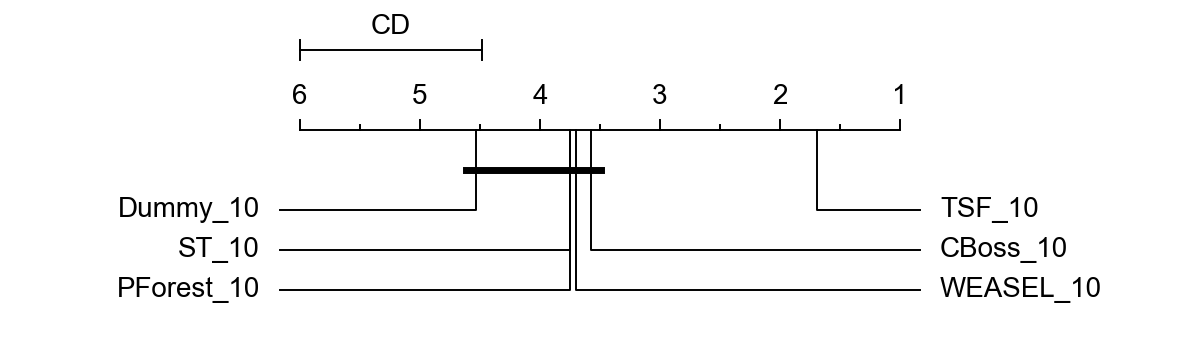
\includegraphics[width=0.49\textwidth]{./Chapters/06 Results/cd_f_score_across_10pct_with_dummy.png} & & 
    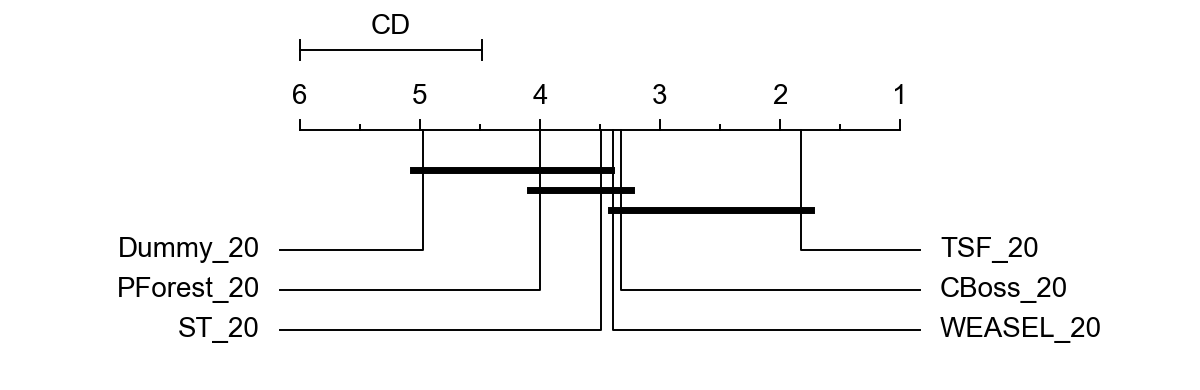
\includegraphics[width=0.40\textwidth]{./Chapters/06 Results/cd_f_score_across_20pct_with_dummy.png} \\
    \textbf{(a) 10\% chunk} & & \textbf{(b) 20\% chunk} \\[6pt]
    \end{tabular}
    \begin{tabular}{ccc}
    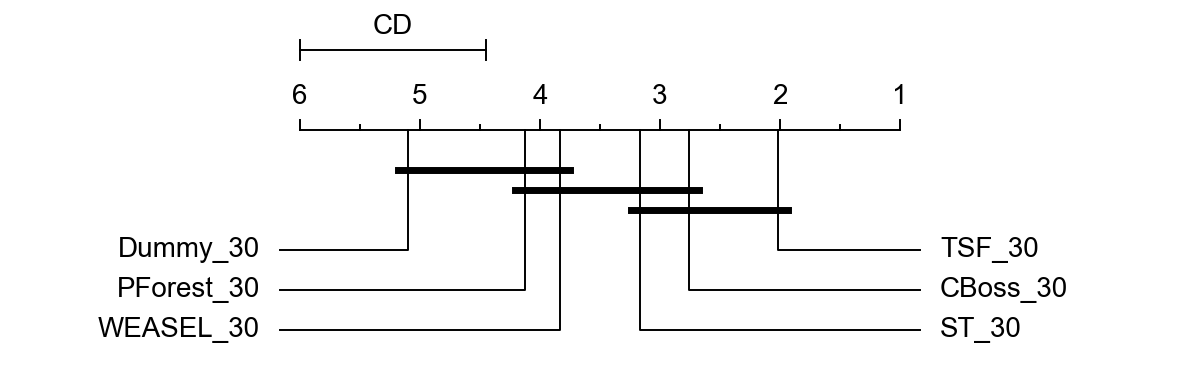
\includegraphics[width=0.49\textwidth]{./Chapters/06 Results/cd_f_score_across_30pct_with_dummy.png} & & 
    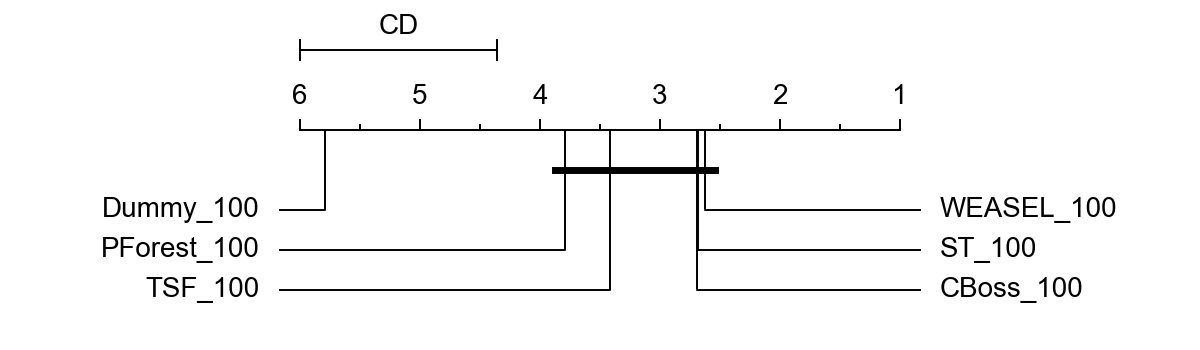
\includegraphics[width=0.49\textwidth]{./Chapters/06 Results/cd_f_score_across_100pct_with_dummy.png} \\
    \textbf{(c) 30\% chunk} & & \textbf{(d) 100\% chunk}  \\[6pt]
    \end{tabular}
    \caption{Critical Difference diagrams per chunk across all classifiers}
  \end{figure}

  \begin{figure} [!htb]
    \centering
    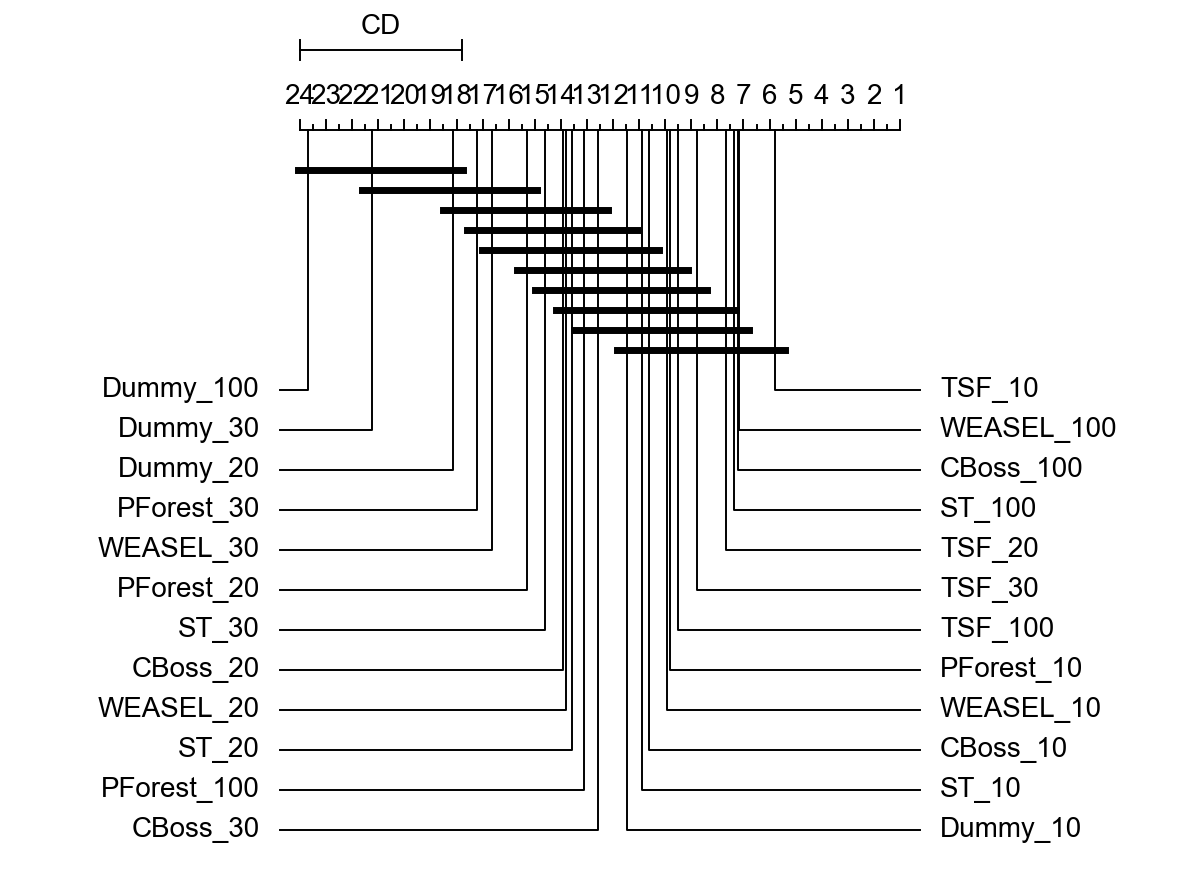
\includegraphics[width=\textwidth]{./Chapters/06 Results/cd_f_score_all_pct_all_clf_dummy.png}
    \caption{Critical Difference diagram for all classifiers and all chunks ($F_{\beta}$)}
  \end{figure}

  \begin{figure} [!htb]
    \centering
    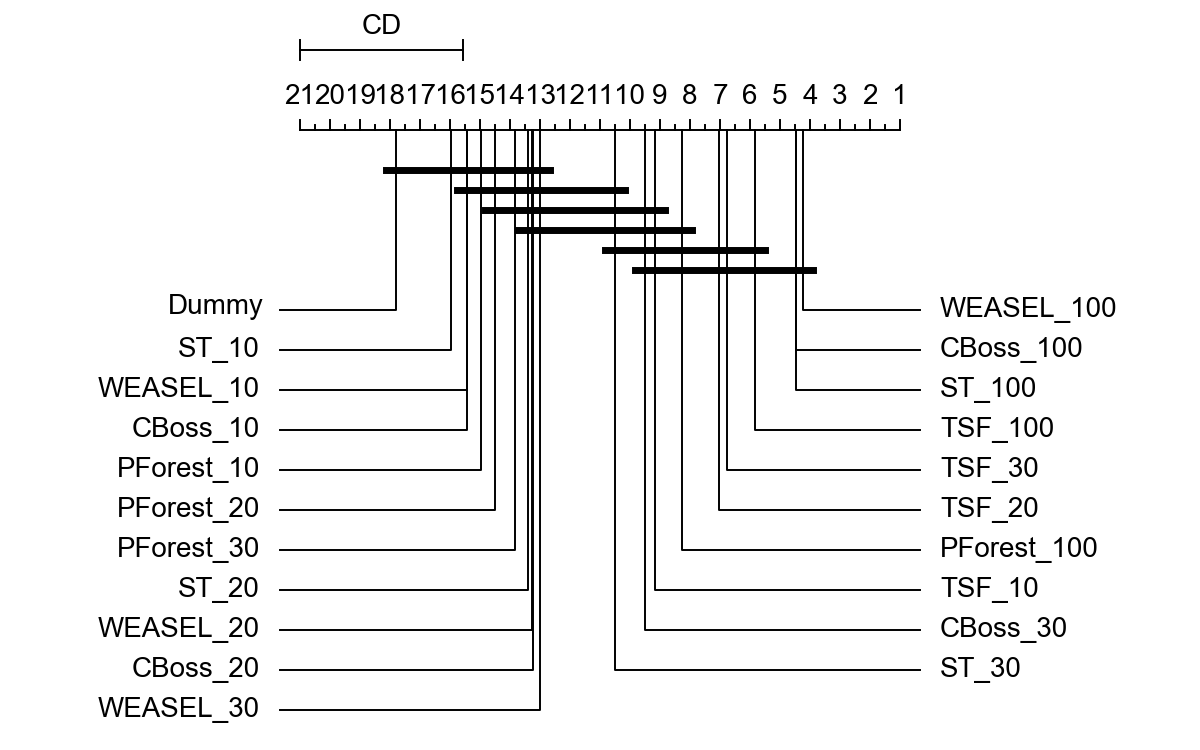
\includegraphics[width=\textwidth]{./Chapters/06 Results/cd_accuracy_all_pct_all_clf_dummy.png}
    \caption{Critical Difference diagram for all classifiers and all chunks (balanced accuracy)}
  \end{figure}

  \section{Data Set characteristics and performance in early classification context}
  \label{AppendixDataCharacteristis}
        \begin{table}[!ht]
            \setlength\extrarowheight{2pt} % for a bit of visual "breathing space"
            \begin{tabularx}{\textwidth}{|X|X|X|X|X|X|X|}
            \hline
            \textbf{Train Length} & \textbf{\#Data sets} & \textbf{CBoss} & \textbf{PForest} & \textbf{ST} & \textbf{TSF} & \textbf{WEASEL} \\ \hline
                1-50 & 3 & 33.33\% & 66.67\% & 33.33\% & 100.00\% & 33.33\% \\ \hline
                51-100 & 5 & 40.00\% & 80.00\% & 60.00\% & 100.00\% & 80.00\% \\ \hline
                101-250 & 7 & 85.71\% & 85.71\% & 100.00\% & 100.00\% & 57.14\% \\ \hline
                251-500 & 8 & 75.00\% & 87.50\% & 75.00\% & 100.00\% & 87.50\% \\ \hline
                501-1000 & 10 & 80.00\% & 80.00\% & 50.00\% & 80.00\% & 60.00\% \\ \hline
                1001+ & 3 & 100.00\% & 33.33\% & 66.67\% & 100.00\% & 66.67\% \\ \hline
            \end{tabularx}
            \caption{Performance of classifiers with respect to length in comparison to baseline on 20\% chunk data sets}
        \end{table}

        \begin{table}[!ht]
            \setlength\extrarowheight{2pt} % for a bit of visual "breathing space"
            \begin{tabularx}{\textwidth}{|X|X|X|X|X|X|X|}
            \hline
            \textbf{Train Length} & \textbf{\#Data sets} & \textbf{CBoss} & \textbf{PForest} & \textbf{ST} & \textbf{TSF} & \textbf{WEASEL} \\ \hline
                1-50 & 3 & 100.00\% & 66.67\% & 100.00\% & 100.00\% & 33.33\%\\ \hline
                51-100 & 5 & 80.00\% & 80.00\% & 100.00\% & 100.00\% & 80.00\% \\ \hline
                101-250 & 7 & 100.00\% & 71.43\% & 100.00\% & 100.00\% & 71.43\% \\ \hline
                251-500 & 8 & 87.50\% & 50.00\% & 75.00\% & 100.00\% & 62.50\% \\ \hline
                501-1000 & 10 &70.00\% & 60.00\% & 60.00\% & 80.00\% & 60.00\% \\ \hline
                1001+ & 3 & 100.00\% & 33.33\% & 66.67\% & 100.00\% & 66.67\% \\ \hline
            \end{tabularx}
            \caption{Performance of classifiers with respect to length in comparison to baseline on 30\% chunk data sets}
        \end{table}

        \begin{table}[!ht]
            \setlength\extrarowheight{2pt} % for a bit of visual "breathing space"
            \begin{tabularx}{\textwidth}{|X|X|X|X|X|X|X|}
            \hline
            \textbf{Train Length} & \textbf{\#Data sets} & \textbf{CBoss} & \textbf{PForest} & \textbf{ST} & \textbf{TSF} & \textbf{WEASEL} \\ \hline
                1-50 & 3 & 100.00\% & 66.67\% & 100.00\% & 100.00\% & 100.00\% \\ \hline
                51-100 & 5 & 100.00\% & 100.00\% & 100.00\% & 100.00\% & 100.00\% \\ \hline
                101-250 & 7 & 100.00\% & 100.00\% & 100.00\% & 100.00\% & 100.00\% \\ \hline
                251-500 & 8 & 100.00\% & 100.00\% & 100.00\% & 100.00\% & 100.00\% \\ \hline
                501-1000 & 10 &80.00\% & 90.00\% & 90.00\% & 80.00\% & 80.00\% \\ \hline
                1001+ & 3 & 100.00\% & 66.67\% & 100.00\% & 100.00\% & 100.00\% \\ \hline
            \end{tabularx}
            \caption{Performance of classifiers with respect to length in comparison to baseline on 100\% chunk data sets}
        \end{table}
    
        \begin{table}[!ht]
            \setlength\extrarowheight{2pt} % for a bit of visual "breathing space"
            \begin{tabularx}{\textwidth}{|X|X|X|X|X|X|X|}
            \hline
            \textbf{Train Size} & \textbf{\#Data sets} & \textbf{CBoss} & \textbf{PForest} & \textbf{ST} & \textbf{TSF} & \textbf{WEASEL} \\ \hline
                1-50 & 14 & 50.00\% & 64.29\% & 50.00\% & 92.86\% & 57.14\% \\ \hline
                51-100 & 9 & 66.67\% & 55.56\% & 44.44\% & 77.78\% & 55.56\% \\ \hline
                101-250 & 7 & 57.14\% & 57.14\% & 71.43\% & 100.00\% & 42.86\% \\ \hline
                251-500 & 4 & 50.00\% & 75.00\% & 75.00\% & 75.00\% & 25.00\% \\ \hline
                501-1000 & 2 &50.00\% & 50.00\% & 100.00\% & 100.00\% & 50.00\% \\ \hline
            \end{tabularx}
            \caption{Performance of classifiers with respect to train size in comparison to baseline on 10\% chunk data sets}
        \end{table}
        
        \begin{table}[!ht]
            \setlength\extrarowheight{2pt} % for a bit of visual "breathing space"
            \begin{tabularx}{\textwidth}{|X|X|X|X|X|X|X|}
            \hline
            \textbf{Train Size} & \textbf{\#Data sets} & \textbf{CBoss} & \textbf{PForest} & \textbf{ST} & \textbf{TSF} & \textbf{WEASEL} \\ \hline
                1-50 & 14 & 71.43\% & 78.57\% & 64.29\% & 92.86\% & 71.43\% \\ \hline
                51-100 & 9 & 77.78\% & 88.89\% & 55.56\% & 100.00\% & 66.67\% \\ \hline
                101-250 & 7 & 71.43\% & 71.43\% & 71.43\% & 100.00\% & 85.71\% \\ \hline
                251-500 & 4 & 75.00\% & 75.00\% & 75.00\% & 75.00\% & 50.00\% \\ \hline
                501-1000 & 2 &50.00\% & 50.00\% & 100.00\% & 100.00\% & 0.00\% \\ \hline
            \end{tabularx}
            \caption{Performance of classifiers with respect to train size in comparison to baseline on 20\% chunk data sets}
        \end{table}
        
        \begin{table}[!ht]
            \setlength\extrarowheight{2pt} % for a bit of visual "breathing space"
            \begin{tabularx}{\textwidth}{|X|X|X|X|X|X|X|}
            \hline
            \textbf{Train Size} & \textbf{\#Data sets} & \textbf{CBoss} & \textbf{PForest} & \textbf{ST} & \textbf{TSF} & \textbf{WEASEL} \\ \hline
                1-50 & 14 & 92.86\% & 71.43\% & 85.71\% & 92.86\% & 71.43\% \\ \hline
                51-100 & 9 & 77.78\% & 55.56\% & 55.56\% & 100.00\% & 55.56\% \\ \hline
                101-250 & 7 & 85.71\% & 57.14\% & 100.00\% & 100.00\% & 85.71\% \\ \hline
                251-500 & 4 & 75.00\% & 50.00\% & 75.00\% & 75.00\% & 50.00\% \\ \hline
                501-1000 & 2 &100.00\% & 50.00\% & 100.00\% & 100.00\% & 0.00\% \\ \hline
            \end{tabularx}
            \caption{Performance of classifiers with respect to train size in comparison to baseline on 30\% chunk data sets}
        \end{table}
        
        \begin{table}[!ht]
            \setlength\extrarowheight{2pt} % for a bit of visual "breathing space"
            \begin{tabularx}{\textwidth}{|X|X|X|X|X|X|X|}
            \hline
            \textbf{Train Size} & \textbf{\#Data sets} & \textbf{CBoss} & \textbf{PForest} & \textbf{ST} & \textbf{TSF} & \textbf{WEASEL} \\ \hline
                1-50 & 14 & 92.86\% & 92.86\% & 100.00\% & 92.86\% & 92.86\% \\ \hline
                51-100 & 9 & 100.00\% & 100.00\% & 100.00\% & 100.00\% & 100.00\% \\ \hline
                101-250 & 7 & 100.00\% & 71.43\% & 100.00\% & 100.00\% & 100.00\% \\ \hline
                251-500 & 4 & 75.00\% & 100.00\% & 75.00\% & 75.00\% & 75.00\% \\ \hline
                501-1000 & 2 &100.00\% & 100.00\% & 100.00\% & 100.00\% & 100.00\% \\ \hline
            \end{tabularx}
            \caption{Performance of classifiers with respect to train size in comparison to baseline on 100\% chunk data sets}
        \end{table}
    
        
\begin{table}[!htb]
	\setlength\extrarowheight{2pt} % for a bit of visual "breathing space"
	\begin{tabularx}{\textwidth}{|X|X|X|X|X|X|X|}
	\hline
	\textbf{Type} & \textbf{\#Data sets} & \textbf{CBoss} & \textbf{PForest} & \textbf{ST} & \textbf{TSF} & \textbf{WEASEL} \\ \hline
		ECG & 5 & 40.00\% & 100.00\% & 80.00\% & 80.00\% & 60.00\% \\ \hline
		SPECTRO & 8 &50.00\% & 37.50\% & 62.50\% & 100.00\% & 12.50\% \\ \hline
		SENSOR & 13 & 53.85\% & 53.85\% & 46.15\% & 76.92\% & 61.54\% \\ \hline
		Traffic & 1 & 0.00\% & 0.00\% & 0.00\% & 100.00\% & 0.00\% \\ \hline
		DEVICE & 5 & 80.00\% & 100.00\% & 100.00\% & 100.00\% & 60.00\% \\ \hline
		EPG & 2 & 100.00\% & 100.00\% & 0.00\% & 100.00\% & 100.00\% \\ \hline
		HAR & 1 & 0.00\% & 0.00\% & 0.00\% & 100.00\% & 0.00\% \\ \hline
		SOUND & 1 & 100.00\% & 0.00\% & 100.00\% & 100.00\% & 100.00\% \\ \hline
  \caption{Performance of classifiers with respect to problem type in comparison to baseline on 10\% chunk data sets}
  \end{tabularx}
\end{table}

\begin{table}[!htb]
	\setlength\extrarowheight{2pt} % for a bit of visual "breathing space"
	\begin{tabularx}{\textwidth}{|X|X|X|X|X|X|X|}
	\hline
	\textbf{Type} & \textbf{\#Data sets} & \textbf{CBoss} & \textbf{PForest} & \textbf{ST} & \textbf{TSF} & \textbf{WEASEL} \\ \hline
		ECG & 5 & 40.00\% & 100.00\% & 80.00\% & 80.00\% & 60.00\% \\ \hline
		SPECTRO & 8 &62.50\% & 62.50\% & 75.00\% & 100.00\% & 37.50\% \\ \hline
		SENSOR & 13 & 76.92\% & 76.92\% & 53.85\% & 92.31\% & 76.92\% \\ \hline
		Traffic & 1 & 100.00\% & 100.00\% & 100.00\% & 100.00\% & 0.00\% \\ \hline
		DEVICE & 5 & 100.00\% & 100.00\% & 100.00\% & 100.00\% & 80.00\% \\ \hline
		EPG & 2 & 100.00\% & 100.00\% & 0.00\% & 100.00\% & 100.00\% \\ \hline
		HAR & 1 & 0.00\% & 0.00\% & 0.00\% & 100.00\% & 100.00\% \\ \hline
		SOUND & 1 & 100.00\% & 0.00\% & 100.00\% & 100.00\% & 100.00\% \\ \hline
  \caption{Performance of classifiers with respect to problem type in comparison to baseline on 20\% chunk data sets}
  \end{tabularx}
\end{table}

\begin{table}[!htb]
	\setlength\extrarowheight{2pt} % for a bit of visual "breathing space"
	\begin{tabularx}{\textwidth}{|X|X|X|X|X|X|X|}
	\hline
	\textbf{Type} & \textbf{\#Data sets} & \textbf{CBoss} & \textbf{PForest} & \textbf{ST} & \textbf{TSF} & \textbf{WEASEL} \\ \hline
		ECG & 5 & 60.00\% & 40.00\% & 100.00\% & 80.00\% & 60.00\% \\ \hline
		SPECTRO & 8 &87.50\% & 25.00\% & 87.50\% & 100.00\% & 37.50\% \\ \hline
		SENSOR & 13 & 84.62\% & 76.92\% & 69.23\% & 92.31\% & 69.23\% \\ \hline
		Traffic & 1 & 100.00\% & 100.00\% & 100.00\% & 100.00\% & 0.00\% \\ \hline
		DEVICE & 5 & 100.00\% & 100.00\% & 100.00\% & 100.00\% & 80.00\% \\ \hline
		EPG & 2 & 100.00\% & 100.00\% & 0.00\% & 100.00\% & 100.00\% \\ \hline
		HAR & 1 & 100.00\% & 0.00\% & 100.00\% & 100.00\% & 100.00\% \\ \hline
		SOUND & 1 & 100.00\% & 0.00\% & 100.00\% & 100.00\% & 100.00\% \\ \hline
  \caption{Performance of classifiers with respect to problem type in comparison to baseline on 30\% chunk data sets}
  \end{tabularx}
\end{table}

\begin{table}[!htb]
	\setlength\extrarowheight{2pt} % for a bit of visual "breathing space"
	\begin{tabularx}{\textwidth}{|X|X|X|X|X|X|X|}
	\hline
	\textbf{Type} & \textbf{\#Data sets} & \textbf{CBoss} & \textbf{PForest} & \textbf{ST} & \textbf{TSF} & \textbf{WEASEL} \\ \hline
		ECG & 5 & 80.00\% & 80.00\% & 100.00\% & 80.00\% & 80.00\% \\ \hline
		SPECTRO & 8 &100.00\% & 100.00\% & 100.00\% & 100.00\% & 100.00\% \\ \hline
		SENSOR & 13 & 92.31\% & 100.00\% & 92.31\% & 92.31\% & 92.31\% \\ \hline
		Traffic & 1 & 100.00\% & 100.00\% & 100.00\% & 100.00\% & 100.00\% \\ \hline
		DEVICE & 5 & 100.00\% & 100.00\% & 100.00\% & 100.00\% & 100.00\% \\ \hline
		EPG & 2 & 100.00\% & 100.00\% & 100.00\% & 100.00\% & 100.00\% \\ \hline
		HAR & 1 & 100.00\% & 0.00\% & 100.00\% & 100.00\% & 100.00\% \\ \hline
		SOUND & 1 & 100.00\% & 0.00\% & 100.00\% & 100.00\% & 100.00\% \\ \hline
  \caption{Performance of classifiers with respect to problem type in comparison to baseline on 100\% chunk data sets}
  \end{tabularx}
\end{table}


\begin{table}[!htb]
	\setlength\extrarowheight{2pt} % for a bit of visual "breathing space"
	\begin{tabularx}{\textwidth}{|X|X|X|X|X|X|X|}
	\hline
	\textbf{\#Classes} & \textbf{\#Data sets} & \textbf{CBoss} & \textbf{PForest} & \textbf{ST} & \textbf{TSF} & \textbf{WEASEL} \\ \hline
		2 & 20 & 40.00\% & 55.00\% & 55.00\% & 90.00\% & 40.00\% \\ \hline
		3 & 6 & 83.33\% & 100.00\% & 66.67\% & 83.33\% & 83.33\% \\ \hline
		4-5 & 6 & 66.67\% & 66.67\% & 66.67\% & 100.00\% & 33.33\% \\ \hline
		6-10 & 2 & 100.00\% & 50.00\% & 50.00\% & 50.00\% & 100.00\% \\ \hline
		11+ & 2 & 50.00\% & 0.00\% & 50.00\% & 100.00\% & 50.00\% \\ \hline
  \caption{Performance of classifiers with respect to number of classes in comparison to baseline on 10\% chunk data sets}
  \end{tabularx}
\end{table}

\begin{table}[!htb]
	\setlength\extrarowheight{2pt} % for a bit of visual "breathing space"
	\begin{tabularx}{\textwidth}{|X|X|X|X|X|X|X|}
	\hline
	\textbf{\#Classes} & \textbf{\#Data sets} & \textbf{CBoss} & \textbf{PForest} & \textbf{ST} & \textbf{TSF} & \textbf{WEASEL} \\ \hline
		2 & 20 & 65.00\% & 85.00\% & 70.00\% & 95.00\% & 60.00\% \\ \hline
		3 & 6 & 83.33\% & 100.00\% & 50.00\% & 83.33\% & 66.67\% \\ \hline
		4-5 & 6 & 83.33\% & 66.67\% & 83.33\% & 100.00\% & 66.67\% \\ \hline
		6-10 & 2 & 100.00\% & 50.00\% & 50.00\% & 100.00\% & 100.00\% \\ \hline
		11+ & 2 & 50.00\% & 0.00\% & 50.00\% & 100.00\% & 100.00\% \\ \hline
  \caption{Performance of classifiers with respect to number of classes in comparison to baseline on 20\% chunk data sets}
  \end{tabularx}
\end{table}

\begin{table}[!htb]
	\setlength\extrarowheight{2pt} % for a bit of visual "breathing space"
	\begin{tabularx}{\textwidth}{|X|X|X|X|X|X|X|}
	\hline
	\textbf{\#Classes} & \textbf{\#Data sets} & \textbf{CBoss} & \textbf{PForest} & \textbf{ST} & \textbf{TSF} & \textbf{WEASEL} \\ \hline
		2 & 20 & 80.00\% & 75.00\% & 90.00\% & 95.00\% & 65.00\% \\ \hline
		3 & 6 & 83.33\% & 66.67\% & 66.67\% & 83.33\% & 50.00\% \\ \hline
		4-5 & 6 & 100.00\% & 33.33\% & 66.67\% & 100.00\% & 66.67\% \\ \hline
		6-10 & 2 & 100.00\% & 50.00\% & 50.00\% & 100.00\% & 50.00\% \\ \hline
		11+ & 2 & 100.00\% & 0.00\% & 100.00\% & 100.00\% & 100.00\% \\ \hline
  \caption{Performance of classifiers with respect to number of classes in comparison to baseline on 30\% chunk data sets}
  \end{tabularx}
\end{table}

\begin{table}[!htb]
	\setlength\extrarowheight{2pt} % for a bit of visual "breathing space"
	\begin{tabularx}{\textwidth}{|X|X|X|X|X|X|X|}
	\hline
	\textbf{\#Classes} & \textbf{\#Data sets} & \textbf{CBoss} & \textbf{PForest} & \textbf{ST} & \textbf{TSF} & \textbf{WEASEL} \\ \hline
		2 & 20 & 95.00\% & 100.00\% & 95.00\% & 95.00\% & 95.00\% \\ \hline
		3 & 6 & 83.33\% & 83.33\% & 100.00\% & 83.33\% & 83.33\% \\ \hline
		4-5 & 6 & 100.00\% & 100.00\% & 100.00\% & 100.00\% & 100.00\% \\ \hline
		6-10 & 2 & 100.00\% & 100.00\% & 100.00\% & 100.00\% & 100.00\% \\ \hline
		11+ & 2 & 100.00\% & 0.00\% & 100.00\% & 100.00\% & 100.00\% \\ \hline
  \caption{Performance of classifiers with respect to number of classes in comparison to baseline on 100\% chunk data sets}
  \end{tabularx}
\end{table}

\section{Results Within Classifier}
\label{AppendixWithin}
\begin{figure} [!htb]
    \centering
    \begin{tabular}{ccc}
    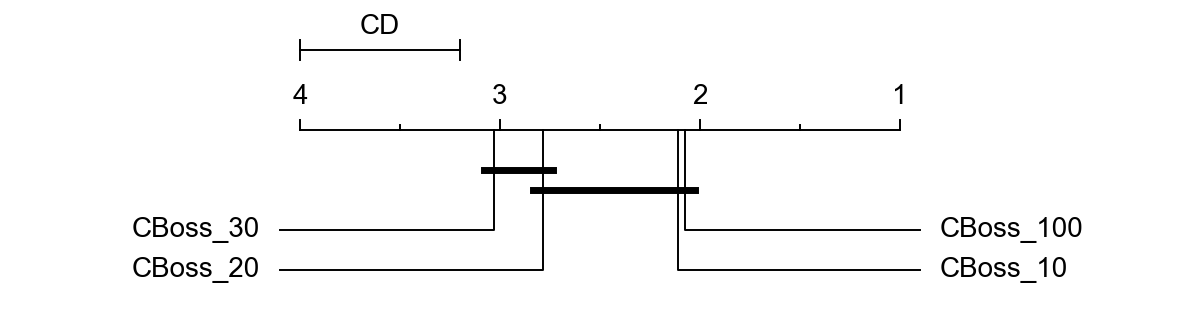
\includegraphics[width=0.49\textwidth]{./Chapters/06 Results/cd_f_score_within_cboss.png} & & 
    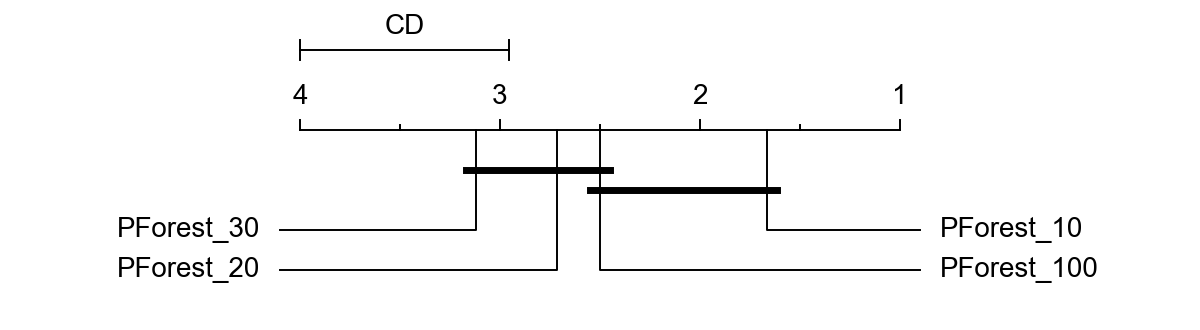
\includegraphics[width=0.40\textwidth]{./Chapters/06 Results/cd_f_score_within_pforest.png} \\
    \textbf{(a) CBoss} & & \textbf{(b) PForest} \\[6pt]
    \end{tabular}
    \begin{tabular}{ccc}
    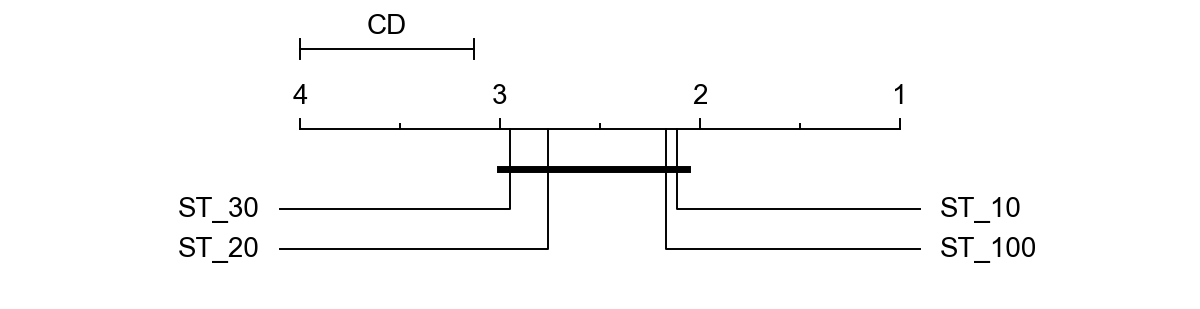
\includegraphics[width=0.49\textwidth]{./Chapters/06 Results/cd_f_score_within_st.png} & & 
    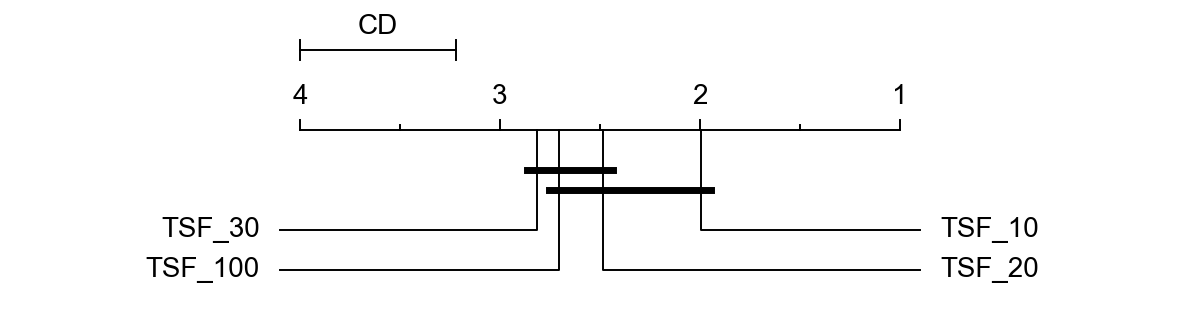
\includegraphics[width=0.49\textwidth]{./Chapters/06 Results/cd_f_score_within_tsf.png} \\
    \textbf{(c) ST} & & \textbf{(d) TSF}  \\[6pt]
    \end{tabular}
    \begin{tabular}{ccc}
    & 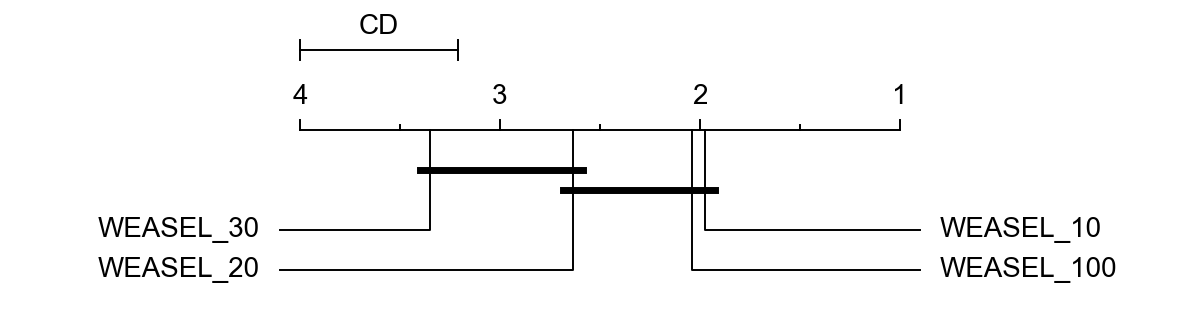
\includegraphics[width=0.49\textwidth]{./Chapters/06 Results/cd_f_score_within_weasel.png} & \\
    & \textbf{(e) WEASEL} & \\[6pt]
    \end{tabular}
    \caption{Crtitical difference diagrams between versions of the same classifier trained on different chunks ($F_{\beta}$)}
\end{figure}

\begin{figure} [!htb]
    \centering
    \begin{tabular}{ccc}
    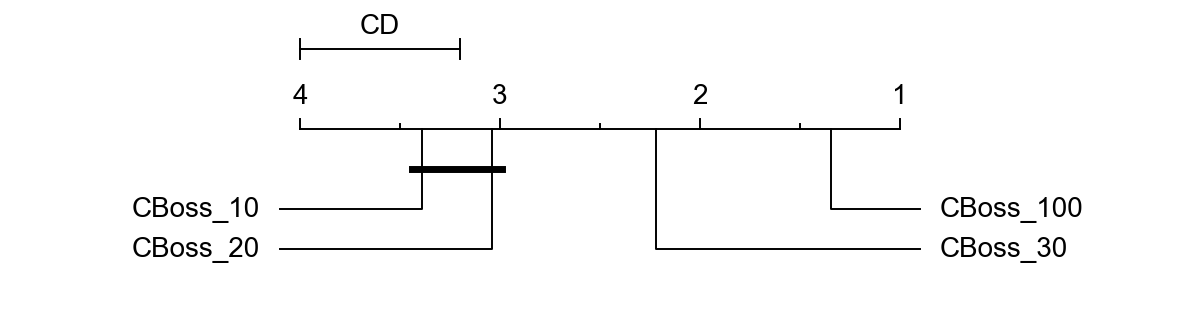
\includegraphics[width=0.49\textwidth]{./Chapters/06 Results/cd_accuracy_within_cboss.png} & & 
    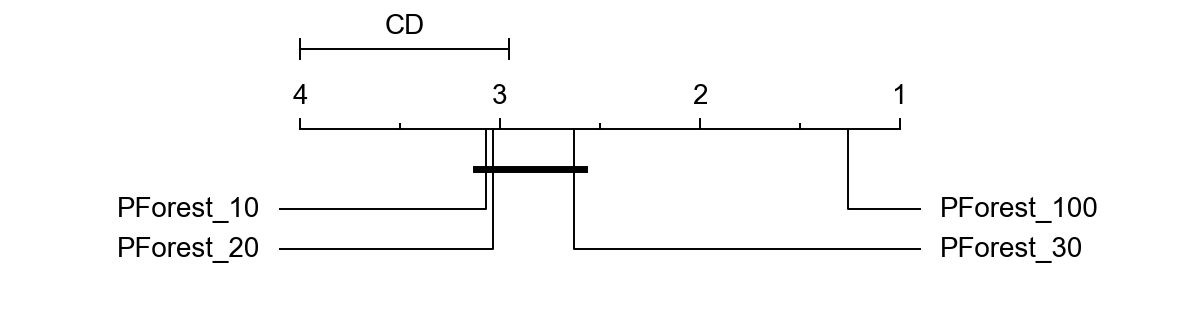
\includegraphics[width=0.40\textwidth]{./Chapters/06 Results/cd_accuracy_within_pforest.png} \\
    \textbf{(a) CBoss} & & \textbf{(b) PForest} \\[6pt]
    \end{tabular}
    \begin{tabular}{ccc}
    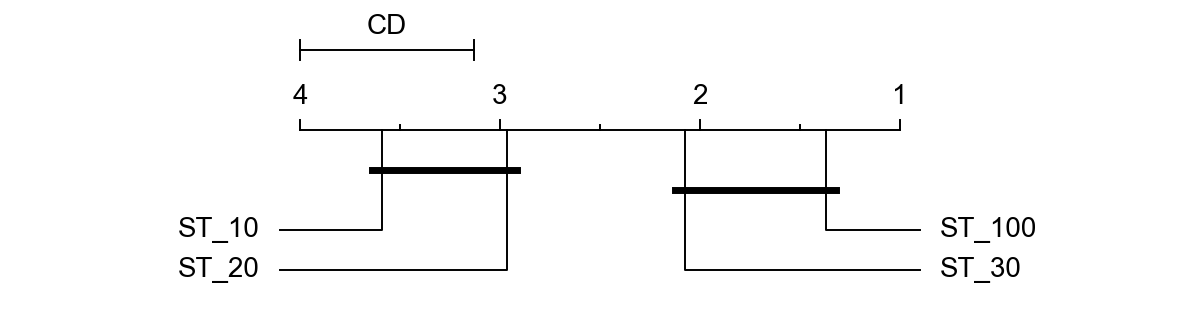
\includegraphics[width=0.49\textwidth]{./Chapters/06 Results/cd_accuracy_within_st.png} & & 
    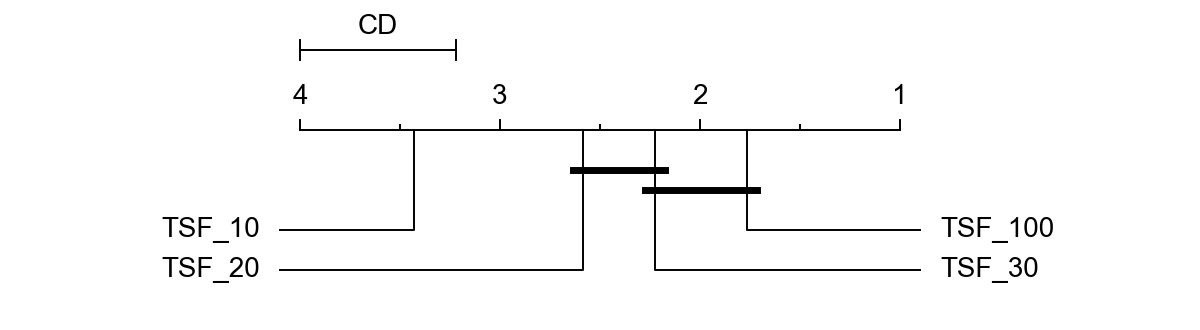
\includegraphics[width=0.49\textwidth]{./Chapters/06 Results/cd_accuracy_within_tsf.png} \\
    \textbf{(c) ST} & & \textbf{(d) TSF}  \\[6pt]
    \end{tabular}
    \begin{tabular}{ccc}
    & 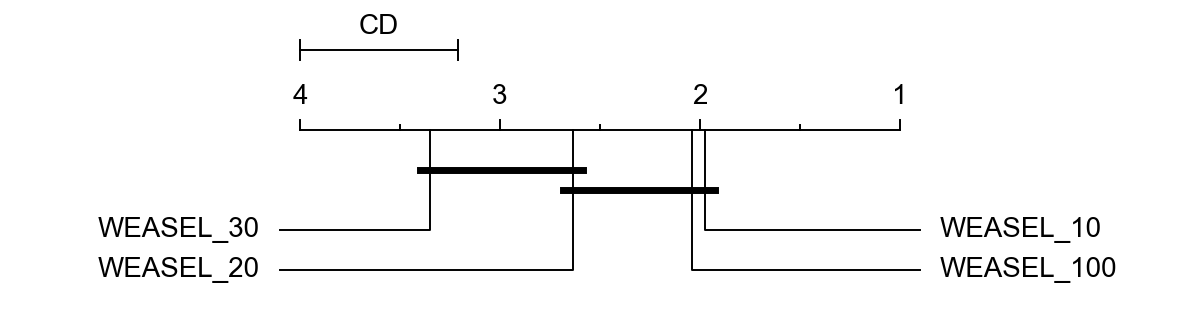
\includegraphics[width=0.49\textwidth]{./Chapters/06 Results/cd_f_score_within_weasel.png} & \\
    & \textbf{(e) WEASEL} & \\[6pt]
    \end{tabular}
    \caption{Crtitical difference diagrams between versions of the same classifier trained on different chunks (balanced accuracy)}
  \end{figure}


\section{Results on Runtime Duration}
\label{AppendixDuration}
  \begin{tiny}
    \begin{landscape}
    {\setlength{\tabcolsep}{1pt}}
    \begin{longtable}{|l|llll|llll|llll|llll|llll|}
        \multirow{2}{*}{\textbf{Data set}} & 
        \multicolumn{4}{c}{\textbf{CBoss}} & \multicolumn{4}{c}{\textbf{PForest}} & \multicolumn{4}{c}{\textbf{ST}} & \multicolumn{4}{c}{\textbf{TSF}} & \multicolumn{4}{c}{\textbf{WEASEL}} \\
        & \textbf{10\%} & \textbf{20\%} & \textbf{30\%} & \textbf{100\%} & \textbf{10\%} & \textbf{20\%} & \textbf{30\%} & \textbf{100\%} & \textbf{10\%} & \textbf{20\%} & \textbf{30\%} & \textbf{100\%} & \textbf{10\%} & \textbf{20\%} & \textbf{30\%} & \textbf{100\%} & \textbf{10\%} & \textbf{20\%} & \textbf{30\%} & \textbf{100\%} \\ [0.5ex]
        \hline
        \endfirsthead % <-- This denotes the end of the header, which will be shown on the first page only
        \hline
        \multirow{2}{*}{\textbf{Data set}} & 
        \multicolumn{4}{c}{\textbf{CBoss}} & \multicolumn{4}{c}{\textbf{PForest}} & \multicolumn{4}{c}{\textbf{ST}} & \multicolumn{4}{c}{\textbf{TSF}} & \multicolumn{4}{c}{\textbf{WEASEL}} \\
        & \textbf{10\%} & \textbf{20\%} & \textbf{30\%} & \textbf{100\%} & \textbf{10\%} & \textbf{20\%} & \textbf{30\%} & \textbf{100\%} & \textbf{10\%} & \textbf{20\%} & \textbf{30\%} & \textbf{100\%} & \textbf{10\%} & \textbf{20\%} & \textbf{30\%} & \textbf{100\%} & \textbf{10\%} & \textbf{20\%} & \textbf{30\%} & \textbf{100\%} \\ [0.5ex]
        \hline
        \endhead % <-- Everything between \endfirsthead and \endhead will be shown as a header on every page
          ACSF1 & 175 & 428 & 779 & 3601 & 15972 & 63002 & 137622 &  & 3969 & 3991 & 4044 & 3919 & 47 & 50 & 58 & 74 & 2 & 11 & 16 & 29 \\ \hline
          AtrialFibrillation & 6 & 18 & 33 & 207 & 506 & 1515 & 3381 & 34266 & 7205 & 7214 & 7213 & 7248 & 75 & 81 & 77 & 98 & 4 & 3 & 4 & 18 \\ \hline
          BasicMotions & 2 & 7 & 16 & 88 & 894 & 993 & 1346 & 8063 &  &  &  &  & 126 & 128 & 131 & 143 & 3 & 6 & 10 & 21 \\ \hline
          Beef & 4 & 12 & 23 & 173 & 350 & 1178 & 2413 & 23595 & 3606 & 3630 & 3641 & 3715 & 27 & 29 & 35 & 44 & 2 & 3 & 3 & 5 \\ \hline
          Car & 7 & 33 & 63 & 559 & 1209 & 3762 & 8142 & 83360 & 3647 & 3662 & 3676 & 3723 & 28 & 34 & 29 & 42 & 4 & 3 & 3 & 14 \\ \hline
          Chinatown & 0 & 0 & 0 & 1 & 18 & 17 & 19 & 51 & 3603 & 3603 & 3603 & 3603 & 39 & 40 & 42 & 43 & 0 & 0 & 0 & 1 \\ \hline
          CinCECGTorso & 18 & 51 & 93 & 596 &  &  &  &  & 3629 & 3654 & 3712 & 3804 & 29 & 32 & 22 & 49 & 1 & 6 & 12 & 23 \\ \hline
          Coffee & 4 & 6 & 19 & 91 & 152 & 303 & 693 & 3456 & 3604 & 3606 & 3607 & 3628 & 36 & 35 & 36 & 40 & 1 & 2 & 4 & 4 \\ \hline
          Computers & 159 & 407 & 334 & 3532 & 3071 & 7870 & 16136 & 146384 & 4242 & 3948 & 3852 & 3883 & 38 & 31 & 41 & 62 & 12 & 15 & 18 & 69 \\ \hline
          Cricket & 433 & 1350 & 1387 & 8110 &  &  &  &  &  &  &  &  & 293 & 308 & 337 & 450 & 61 & 98 & 167 & 623 \\ \hline
          DuckDuckGeese &  &  &  &  &  &  &  &  &  &  &  &  & 8780 & 8996 & 9323 & 10706 &  &  &  &  \\ \hline
          Earthquakes & 112 & 261 & 1006 & 3603 & 5893 & 12552 & 22818 & 198829 & 4182 & 3982 & 3862 & 3750 & 52 & 41 & 48 & 59 & 12 & 12 & 17 & 71 \\ \hline
          ECG200 & 1 & 3 & 17 & 38 & 388 & 517 & 713 & 4431 & 3608 & 3611 & 3613 & 3626 & 32 & 28 & 41 & 21 & 1 & 2 & 3 & 10 \\ \hline
          ECG5000 & 38 & 70 & 85 & 1519 & 1911 & 2200 & 2594 & 11566 & 3638 & 3642 & 3637 & 3687 & 61 & 69 & 67 & 74 & 6 & 14 & 26 & 33 \\ \hline
          ECGFiveDays & 0 & 1 & 3 & 8 & 69 & 109 & 165 & 1240 & 3602 & 3603 & 3605 & 3608 & 23 & 28 & 36 & 40 & 0 & 1 & 2 & 3 \\ \hline
          ElectricDevices & 2622 & 3642 & 3634 & 3749 &  &  &  &  & 4257 & 4697 & 4830 & 3789 & 557 & 567 & 590 & 622 & 87 & 524 & 836 & 3201 \\ \hline
          EOGHorizontalSignal & 661 & 2487 & 3604 & 3618 & 17477 & 60769 & 112039 &  & 3608 & 3604 & 3673 & 3707 & 65 & 69 & 112 & 164 & 36 & 74 & 127 & 786 \\ \hline
          EOGVerticalSignal & 317 & 3114 & 3604 & 3606 &  &  &  &  & 3609 & 3609 & 3670 & 3704 & 47 & 50 & 57 & 151 & 37 & 57 & 109 & 611 \\ \hline
          Epilepsy & 15 & 63 & 126 & 826 &  &  &  &  & 10869 & 10916 & 10988 & 12083 & 135 & 114 & 135 & 157 & 9 & 23 & 39 & 61 \\ \hline
          ERing & 1 & 1 & 3 & 24 & 456 & 534 & 648 & 2436 &  &  &  &  & 145 & 123 & 149 & 146 & 1 & 2 & 4 & 15 \\ \hline
          EthanolConcentration & 1154 & 3376 & 6188 & 10786 &  &  &  &  & 10985 & 11051 & 11105 & 11134 & 241 & 271 & 287 & 566 & 80 & 202 & 355 & 844 \\ \hline
          EthanolLevel & 2774 & 3604 & 3606 & 3631 &  &  &  &  & 3691 & 3701 & 3775 & 3702 & 61 & 65 & 83 & 350 & 33 & 93 & 126 & 679 \\ \hline
          FaceDetection &  &  &  &  &  &  &  &  &  &  &  &  &  &  &  &  & 83 & 321 & 806 &  \\ \hline
          FingerMovements & 27 & 124 & 293 & 1662 &  &  &  &  &  &  &  &  & 323 & 321 & 330 & 341 & 23 & 63 & 114 & 583 \\ \hline
          FordA & 3611 & 3607 & 3643 & 3832 &  &  &  &  & 3760 & 3816 & 3707 & 3841 & 242 & 232 & 326 & 571 & 206 & 210 & 379 & 1425 \\ \hline
          FordB & 3636 & 3711 & 3675 & 3810 &  &  &  &  & 3829 & 3800 & 3771 & 3733 & 188 & 118 & 342 & 527 & 250 & 195 & 480 & 1884 \\ \hline
          FreezerRegularTrain & 15 & 27 & 90 & 592 & 755 & 816 & 1379 & 12258 & 3715 & 3698 & 3661 & 3739 & 35 & 32 & 33 & 39 & 3 & 7 & 7 & 15 \\ \hline
          FreezerSmallTrain & 2 & 3 & 11 & 28 & 131 & 296 & 627 & 5683 & 3605 & 3605 & 3604 & 3610 & 25 & 25 & 26 & 30 & 1 & 3 & 4 & 4 \\ \hline
          Fungi & 1 & 3 & 2 &  & 133 & 297 & 564 & 5261 &  &  &  &  & 30 & 24 & 32 & 37 & 0 & 1 & 2 & 2 \\ \hline
          Ham & 31 & 105 & 211 & 1505 & 1772 & 5044 & 10404 & 104283 & 3665 & 3740 & 3765 & 3909 & 42 & 35 & 32 & 52 & 4 & 6 & 5 & 14 \\ \hline
          HandMovementDirection & 177 & 593 & 889 & 6823 & 11414 & 21094 & 37411 & 321914 &  &  &  &  & 384 & 486 & 502 & 593 & 81 & 203 & 129 & 412 \\ \hline
          Handwriting & 12 & 40 & 67 & 595 &  &  &  &  & 10858 & 10932 & 10987 & 11578 & 134 & 140 & 138 & 153 & 8 & 18 & 30 & 60 \\ \hline
          Heartbeat & 1257 & 3866 & 7667 & 52348 &  &  &  &  &  &  &  &  & 1343 & 1384 & 1409 & 1606 & 21 & 55 & 45 & 189 \\ \hline
          HouseTwenty & 28 & 152 & 134 & 1897 & 5564 & 20665 & 50006 & 435853 & 3697 & 3706 & 3680 & 3761 & 30 & 33 & 35 & 55 & 3 & 7 & 8 & 30 \\ \hline
          InsectEPGRegularTrain & 16 & 46 & 83 & 514 & 524 & 1736 & 3818 & 41925 & 3674 & 3697 & 3696 & 3767 & 40 & 42 & 42 & 52 & 5 & 5 & 7 & 25 \\ \hline
          InsectEPGSmallTrain & 3 & 10 & 17 & 122 & 126 & 426 & 956 & 9921 & 3607 & 3608 & 3614 & 3629 & 24 & 28 & 26 & 33 & 2 & 2 & 2 & 7 \\ \hline
          InsectWingbeatSound & 24 & 33 & 64 & 382 &  &  &  &  & 3650 & 3678 & 3678 & 3714 & 50 & 49 & 51 & 59 & 4 & 8 & 16 & 21 \\ \hline
          ItalyPowerDemand & 0 & 0 & 1 & 2 & 223 & 227 & 211 & 206 & 3604 & 3603 & 3602 & 3608 & 25 & 32 & 32 & 35 & 0 & 0 & 1 & 2 \\ \hline
          LargeKitchenAppliances & 310 & 824 & 1544 & 3604 & 4433 & 12251 & 24973 & 270857 & 4106 & 4014 & 4038 & 4027 & 46 & 45 & 50 & 84 & 22 & 22 & 38 & 164 \\ \hline
          Libras & 1 & 1 & 6 & 60 & 2340 & 2382 & 2390 & 3495 & 7211 & 7235 & 7259 & 7363 & 85 & 88 & 88 & 92 & 1 & 3 & 5 & 23 \\ \hline
          Lightning2 & 8 & 38 & 40 & 593 & 1478 & 5459 & 11789 & 111426 & 3665 & 3721 & 3792 & 3997 & 40 & 28 & 23 & 38 & 5 & 5 & 7 & 21 \\ \hline
          Lightning7 & 6 & 20 & 33 & 110 & 780 & 2058 & 4271 & 42482 & 3636 & 3672 & 3723 & 3757 & 28 & 37 & 40 & 44 & 2 & 4 & 5 & 10 \\ \hline
          LSST & 0 & 956 & 1247 & 7538 &  &  &  &  &  &  &  &  & 698 & 698 & 709 & 733 & 25 & 78 & 152 & 826 \\ \hline
          Meat & 5 & 13 & 24 & 219 & 608 & 1428 & 2924 & 29454 & 3616 & 3626 & 3640 & 3781 & 39 & 28 & 35 & 37 & 3 & 4 & 3 & 9 \\ \hline
          MoteStrain & 1 & 1 & 2 & 10 & 54 & 65 & 88 & 441 & 3602 & 3602 & 3604 & 3616 & 34 & 23 & 23 & 25 & 0 & 0 & 1 & 3 \\ \hline
          MotorImagery & 65994 &  &  &  &  &  &  &  &  &  &  &  & 1874 & 2115 & 2391 & 4483 & 217 & 533 & 806 & 2208 \\ \hline
          NATOPS & 49 & 52 & 114 & 851 & 24792 & 24483 & 24704 & 36247 &  &  &  &  & 1103 & 1108 & 1125 & 1178 & 16 & 39 & 67 & 316 \\ \hline
          NonInvasiveFetalECGThorax1 & 1538 & 6368 & 15200 & 51086 &  &  &  &  & 3645 & 3678 & 3707 & 3812 & 121 & 131 & 146 & 404 & 408 & 477 & 842 & 2395 \\ \hline
          NonInvasiveFetalECGThorax2 & 1479 & 5761 & 13591 & 45878 &  &  &  &  & 3649 & 3679 & 3680 & 3846 & 118 & 130 & 150 & 402 & 272 & 372 & 991 & 2539 \\ \hline
          OliveOil & 5 & 16 & 29 & 180 & 425 & 1389 & 2940 & 24060 & 3613 & 3615 & 3630 & 3674 & 34 & 38 & 41 & 46 & 2 & 1 & 2 & 4 \\ \hline
          PEMS-SF &  &  &  &  &  &  &  &  &  &  &  &  & 9541 & 9759 & 9849 & 10541 &  &  &  &  \\ \hline
          Phoneme & 207 & 1134 & 969 & 3602 & 12344 & 42219 & 91768 & 915733 & 3760 & 3811 & 3815 & 3741 & 56 & 29 & 72 & 91 & 15 & 14 & 48 & 326 \\ \hline
          PigAirwayPressure & 283 & 688 & 1338 & 3601 &  &  &  &  & 3830 & 3967 & 3869 & 3777 & 34 & 38 & 43 & 80 & 17 & 35 & 51 & 741 \\ \hline
          PigArtPressure & 181 & 1049 & 1033 & 3601 &  &  &  &  & 3798 & 3936 & 4020 & 3964 & 39 & 58 & 53 & 102 & 16 & 34 & 57 & 203 \\ \hline
          PigCVP & 197 & 1405 & 1831 & 3601 & 96143 & 380569 &  &  & 3843 & 4007 & 3940 & 3886 & 50 & 39 & 42 & 81 & 13 & 35 & 60 & 261 \\ \hline
          Plane & 5 & 16 & 30 & 143 & 447 & 800 & 1248 & 8822 & 3606 & 3617 & 3632 & 3781 & 37 & 40 & 42 & 42 & 1 & 3 & 4 & 7 \\ \hline
          PowerCons & 5 & 17 & 36 & 138 & 1014 & 1218 & 1361 & 2969 & 3657 & 3792 & 3774 & 3712 & 49 & 39 & 33 & 50 & 1 & 4 & 4 & 12 \\ \hline
          RacketSports & 6 & 10 & 8 & 76 & 4296 & 4130 & 4072 & 4806 &  &  &  &  & 208 & 230 & 266 & 276 & 1 & 3 & 6 & 32 \\ \hline
          RefrigerationDevices & 239 & 410 & 1608 & 3605 & 4721 & 12419 & 25695 & 239726 & 4054 & 4148 & 4046 & 3972 & 56 & 49 & 56 & 61 & 27 & 27 & 47 & 106 \\ \hline
          Rock & 44 & 59 & 237 & 1678 & 4424 & 17372 & 41005 & 475073 & 3648 & 3649 & 3689 & 3789 & 43 & 46 & 54 & 74 & 4 & 4 & 6 & 17 \\ \hline
          ScreenType & 269 & 283 & 1025 & 3606 & 4964 & 13757 &  &  & 4149 & 4072 & 4118 & 4110 & 53 & 65 & 34 & 101 & 20 & 24 & 37 & 288 \\ \hline
          SelfRegulationSCP1 & 1424 & 2340 & 4519 & 21574 &  &  &  &  &  &  &  &  & 342 & 373 & 272 & 589 & 181 & 136 & 192 & 755 \\ \hline
          SelfRegulationSCP2 & 825 & 2693 & 5369 & 25174 & 29494 &  &  &  &  &  &  &  & 419 & 405 & 433 & 524 & 71 & 149 & 238 & 591 \\ \hline
          SemgHandGenderCh2 & 367 & 1331 & 2429 & 3605 &  &  &  &  & 3695 & 3789 & 3774 & 3833 & 58 & 70 & 75 & 163 & 19 & 28 & 72 & 184 \\ \hline
          SemgHandMovementCh2 & 963 & 2976 & 3605 & 3598 &  &  &  &  & 3647 & 3687 & 3731 & 3681 & 114 & 62 & 69 & 246 & 37 & 61 & 76 & 338 \\ \hline
          SemgHandSubjectCh2 & 1900 & 3603 & 3611 & 3610 &  &  &  &  & 3648 & 3802 & 3742 & 3753 & 61 & 73 & 78 & 256 & 28 & 45 & 94 & 529 \\ \hline
          SmallKitchenAppliances & 175 & 941 & 525 & 3602 & 9800 & 27216 & 59998 &  & 3934 & 4007 & 3996 & 4022 & 74 & 46 & 49 & 84 & 16 & 29 & 32 & 393 \\ \hline
          SonyAIBORobotSurface1 & 0 & 1 & 1 & 9 & 43 & 43 & 54 & 260 & 3603 & 3603 & 3604 & 3607 & 32 & 31 & 35 & 35 & 0 & 0 & 0 & 2 \\ \hline
          SonyAIBORobotSurface2 & 0 & 1 & 1 & 6 & 55 & 56 & 72 & 292 & 3603 & 3605 & 3603 & 3607 & 33 & 23 & 24 & 25 & 0 & 0 & 1 & 3 \\ \hline
          StandWalkJump & 69 & 169 & 318 & 2246 & 7699 & 31252 & 69596 &  & 14443 & 14471 & 14491 & 14539 & 170 & 187 & 190 & 274 & 8 & 18 & 25 & 73 \\ \hline
          StarlightCurves & 478 & 1542 & 3258 & 24151 &  &  &  &  & 3676 & 3750 & 3752 & 3792 & 78 & 86 & 99 & 332 & 21 & 31 & 43 & 119 \\ \hline
          Strawberry & 112 & 453 & 448 & 3601 & 4020 & 4948 & 6687 & 41484 & 3649 & 3683 & 3741 & 3781 & 75 & 52 & 53 & 65 & 9 & 19 & 38 & 53 \\ \hline
          Trace & 7 & 27 & 42 & 284 & 977 & 1472 & 2405 & 13619 & 3654 & 3690 & 3657 & 3679 & 31 & 38 & 41 & 33 & 2 & 4 & 5 & 13 \\ \hline
          TwoLeadECG & 0 & 1 & 1 & 7 & 76 & 90 & 104 & 394 & 3602 & 3602 & 3602 & 3604 & 23 & 25 & 24 & 29 & 0 & 1 & 1 & 3 \\ \hline
          UWaveGestureLibrary & 22 & 77 & 129 & 698 &  &  &  &  & 11015 & 11399 & 11599 & 11477 & 126 & 90 & 138 & 145 & 17 & 38 & 61 & 76 \\ \hline
          Wafer & 82 & 235 & 466 & 3605 & 8088 & 9642 & 10263 & 43869 & 3643 & 3696 & 3711 & 3707 & 68 & 67 & 69 & 77 & 6 & 23 & 30 & 47 \\ \hline
          Wine & 2 & 6 & 19 & 120 & 305 & 725 & 1470 & 12827 & 3604 & 3620 & 3630 & 3676 & 26 & 26 & 27 & 34 & 1 & 2 & 2 & 4 \\ \hline
    \caption{Train Time (CPU Time) for all 5 classifiers on 77 data sets for all chunks}
    \label{tab:longduration}
    \end{longtable}
    \end{landscape}
  \end{tiny}
%%%%%%%%%%%%%
  %durations
%%%%%%%%%%%%%
  \begin{figure} [!htb]
    \centering
    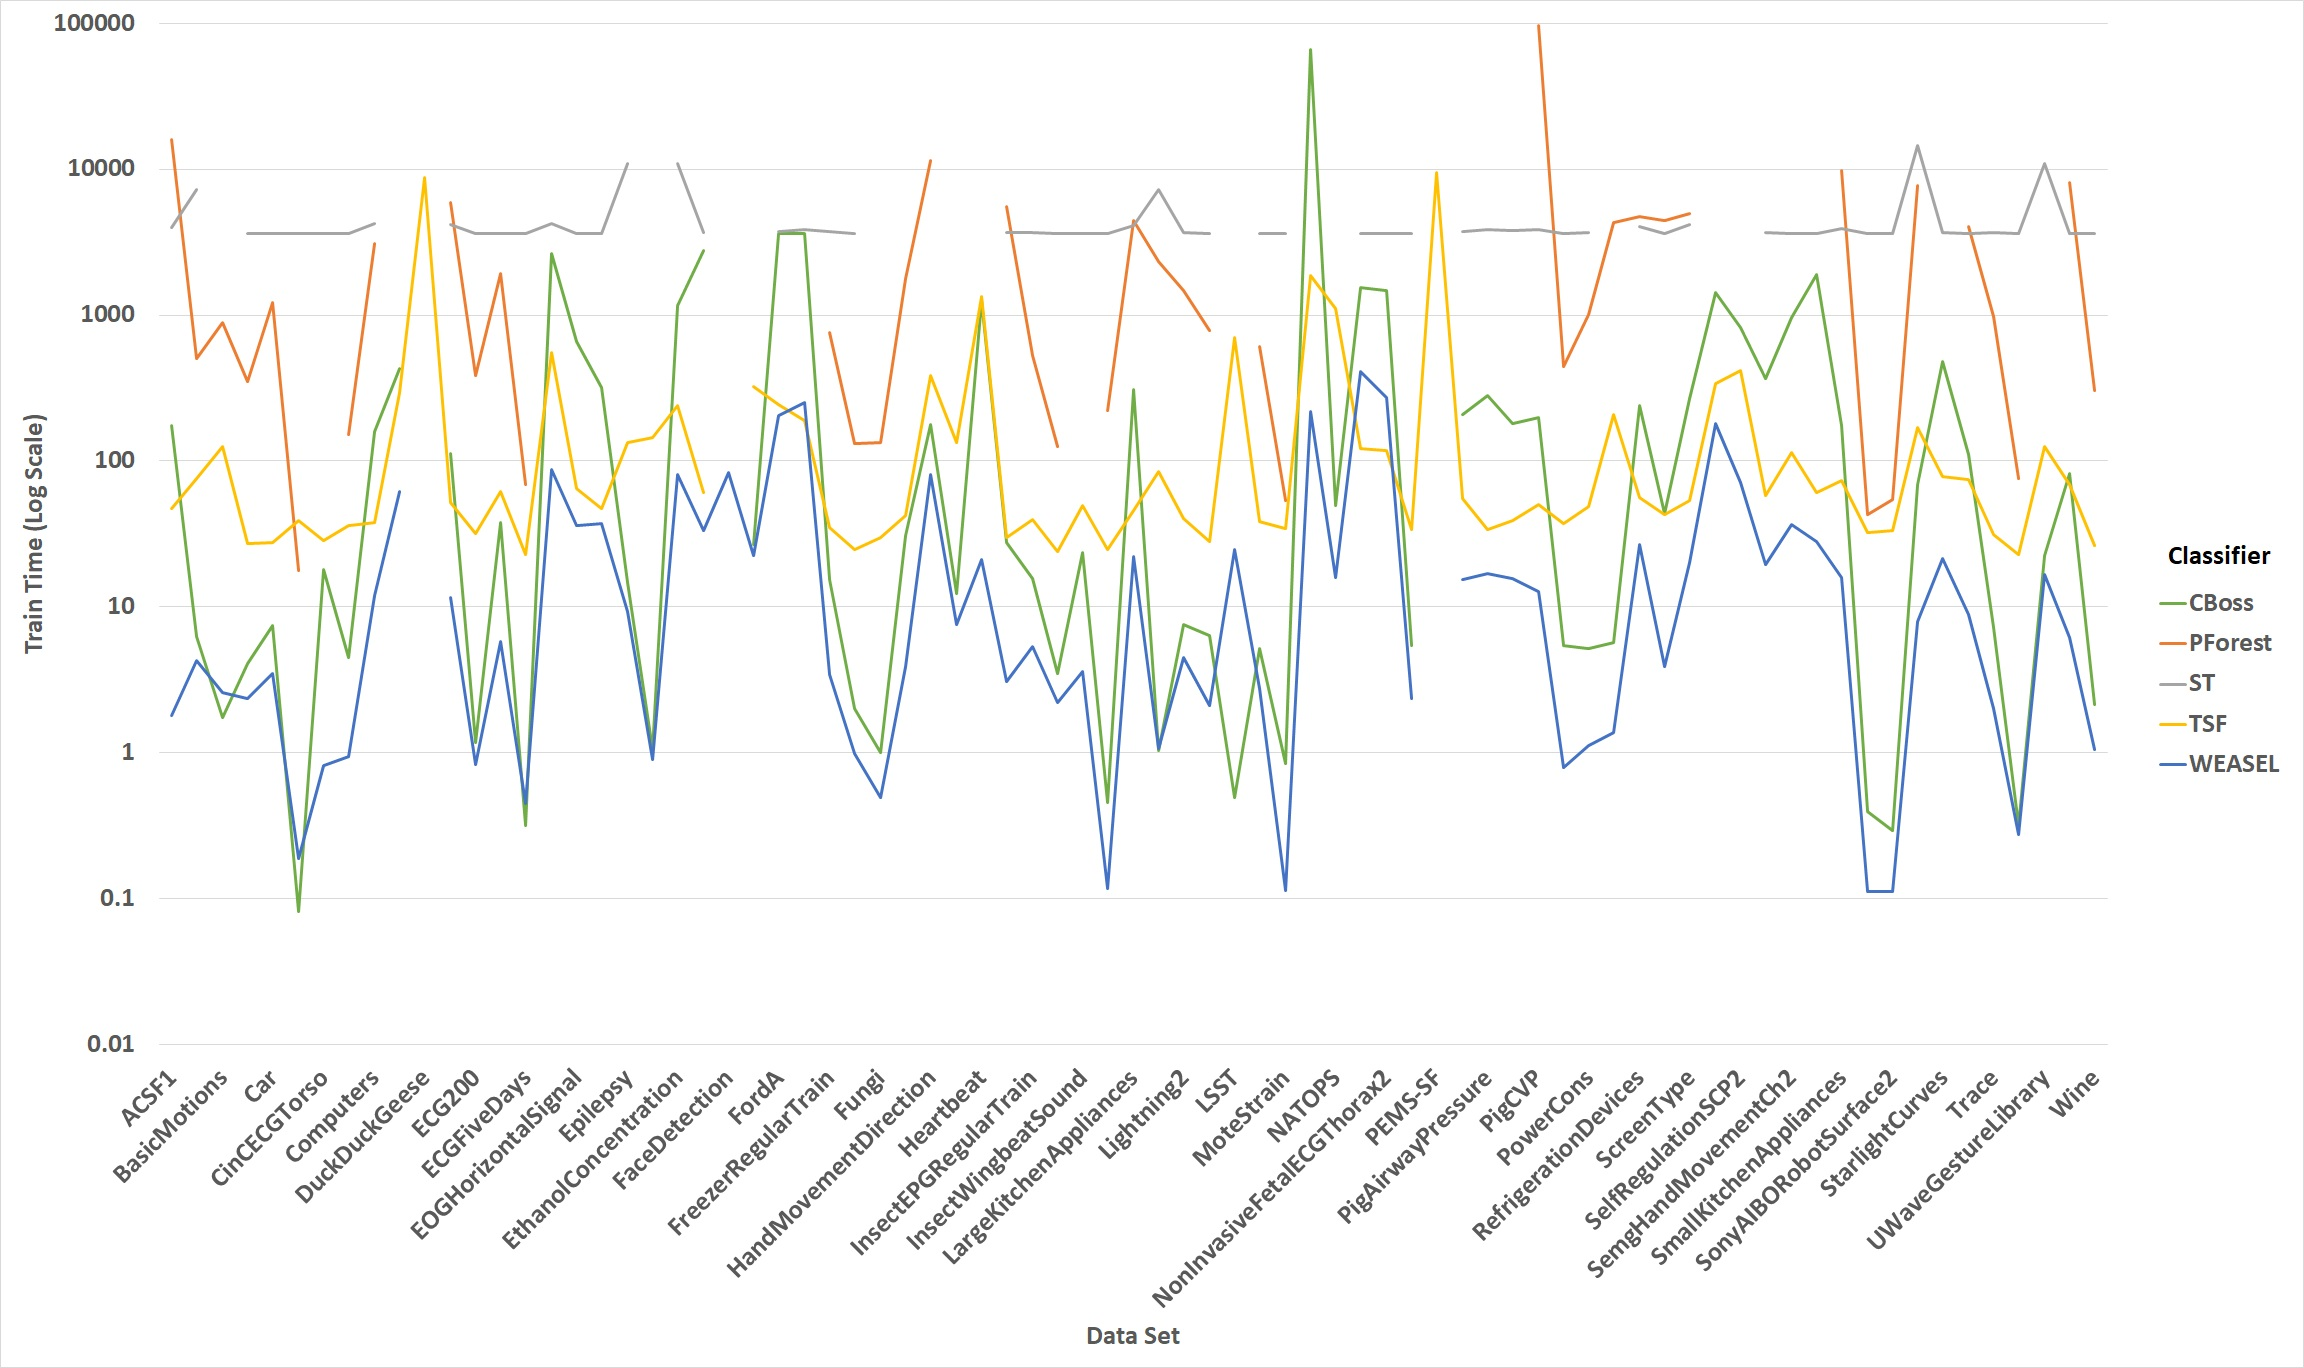
\includegraphics[width=\textwidth]{./Chapters/06 Results/Duration_10pct.jpg}
    \caption{Train Time (CPU Time in Log Scale) for all 5 classifiers for 10\% chunk}
    \label{fig:Duration10Line}
  \end{figure}
  
  \begin{figure} [!htb]
    \centering
    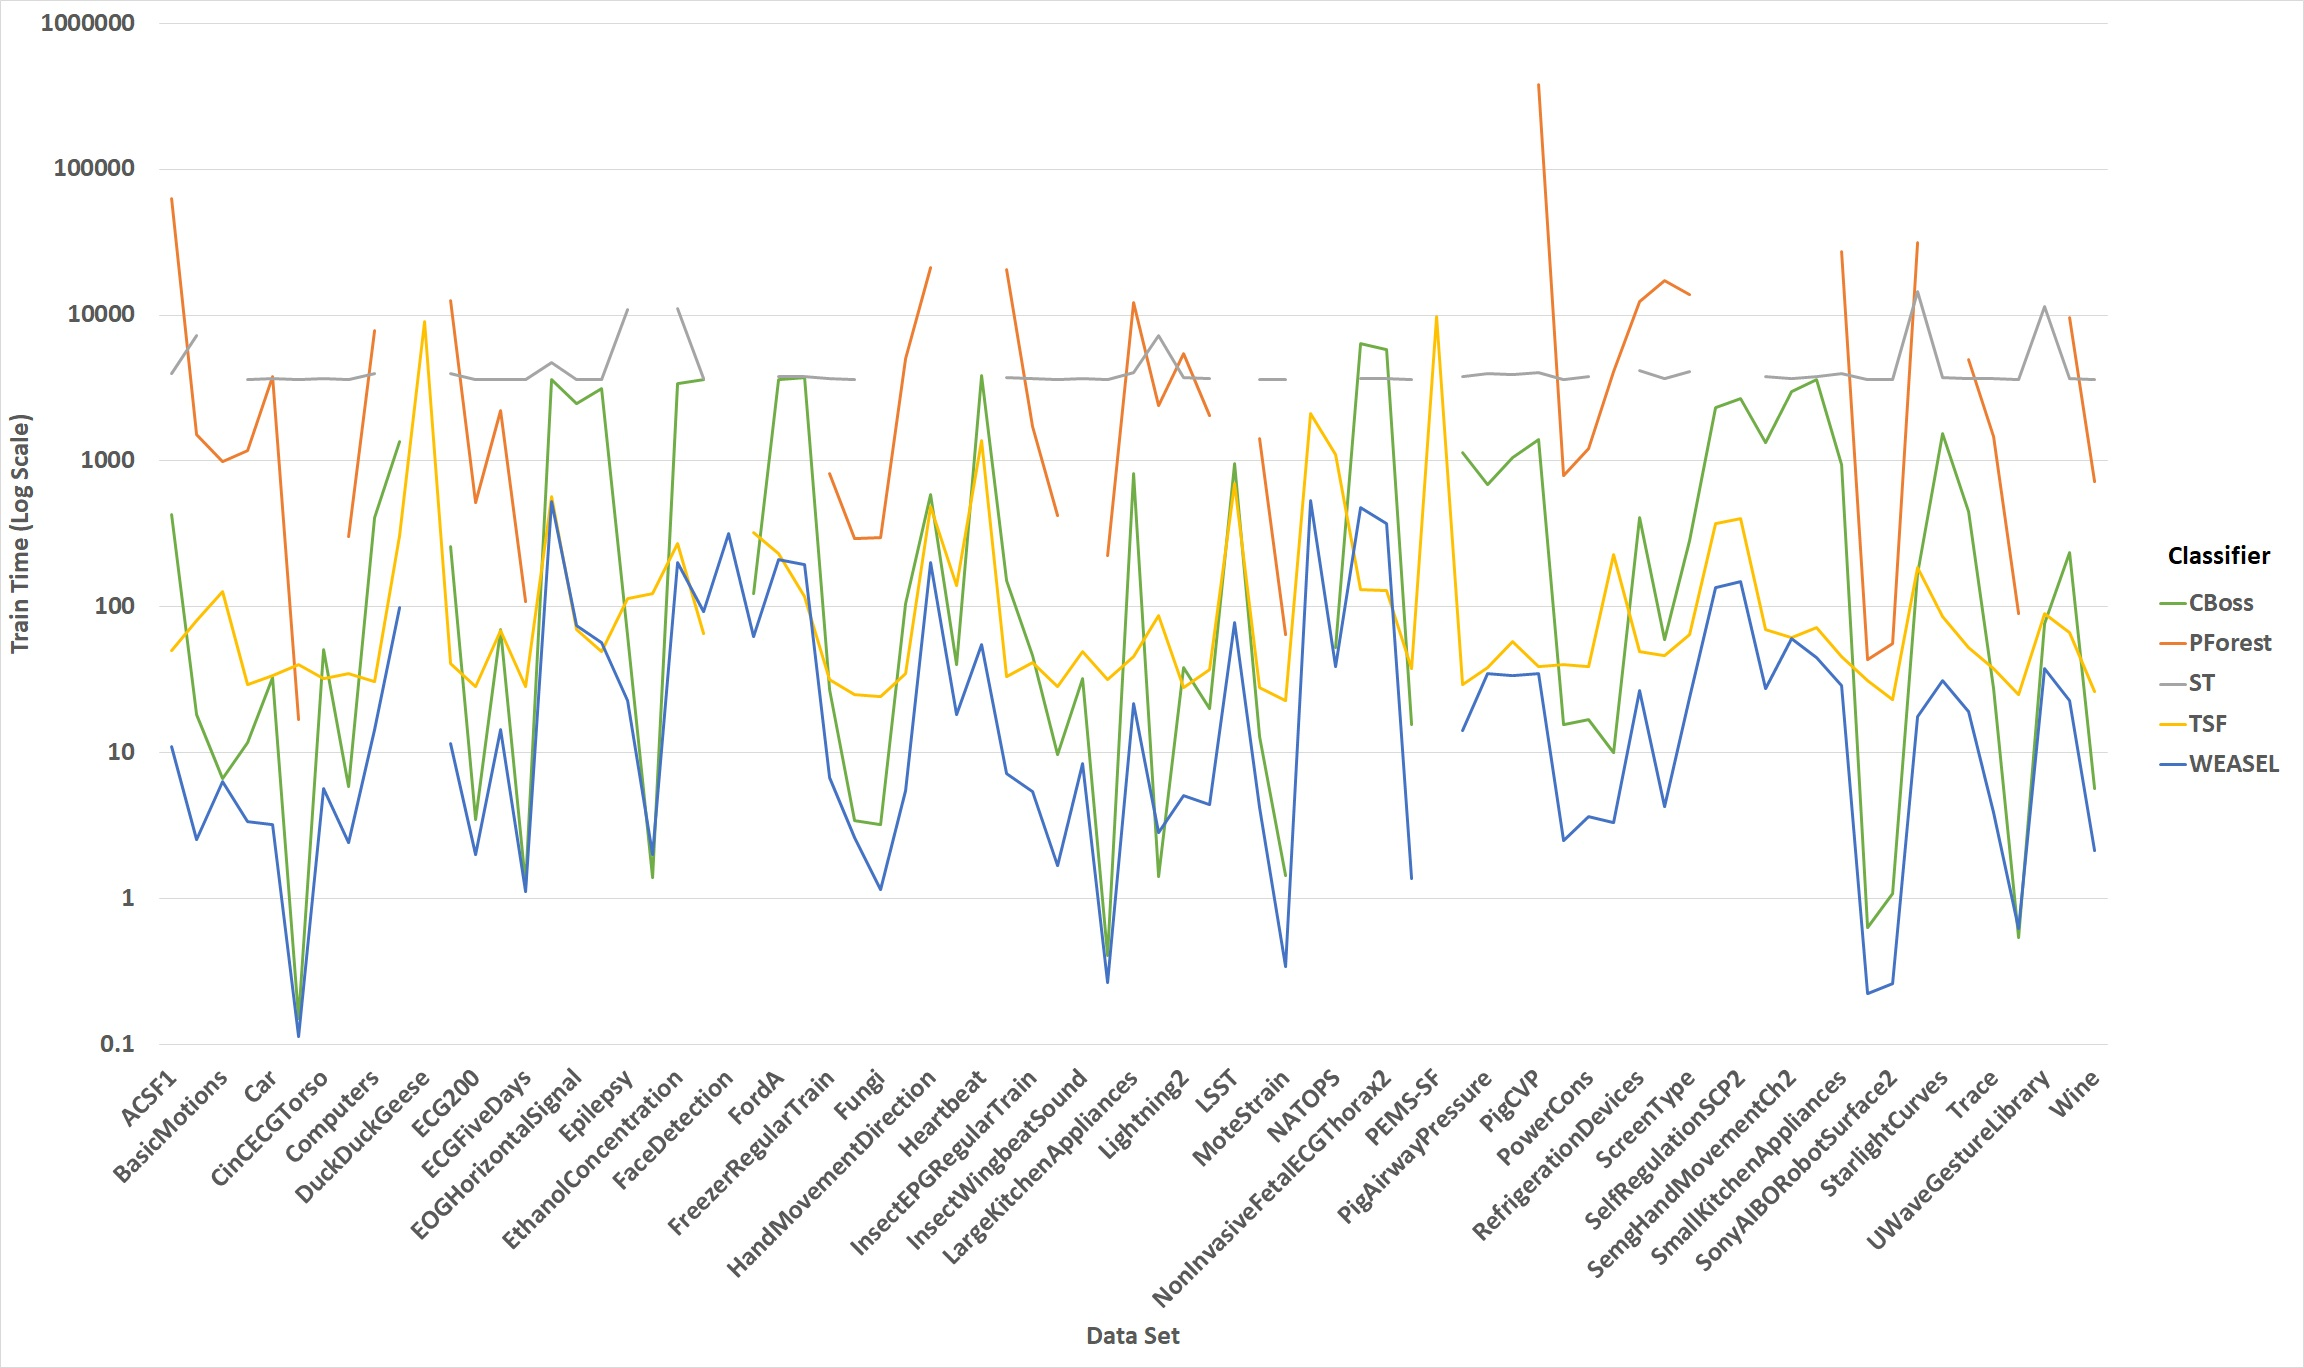
\includegraphics[width=\textwidth]{./Chapters/06 Results/Duration_20pct.jpg}
    \caption{Train Time (CPU Time in Log Scale) for all 5 classifiers for 20\% chunk}
    \label{fig:Duration20Line}
  \end{figure}
  
  \begin{figure} [!htb]
    \centering
    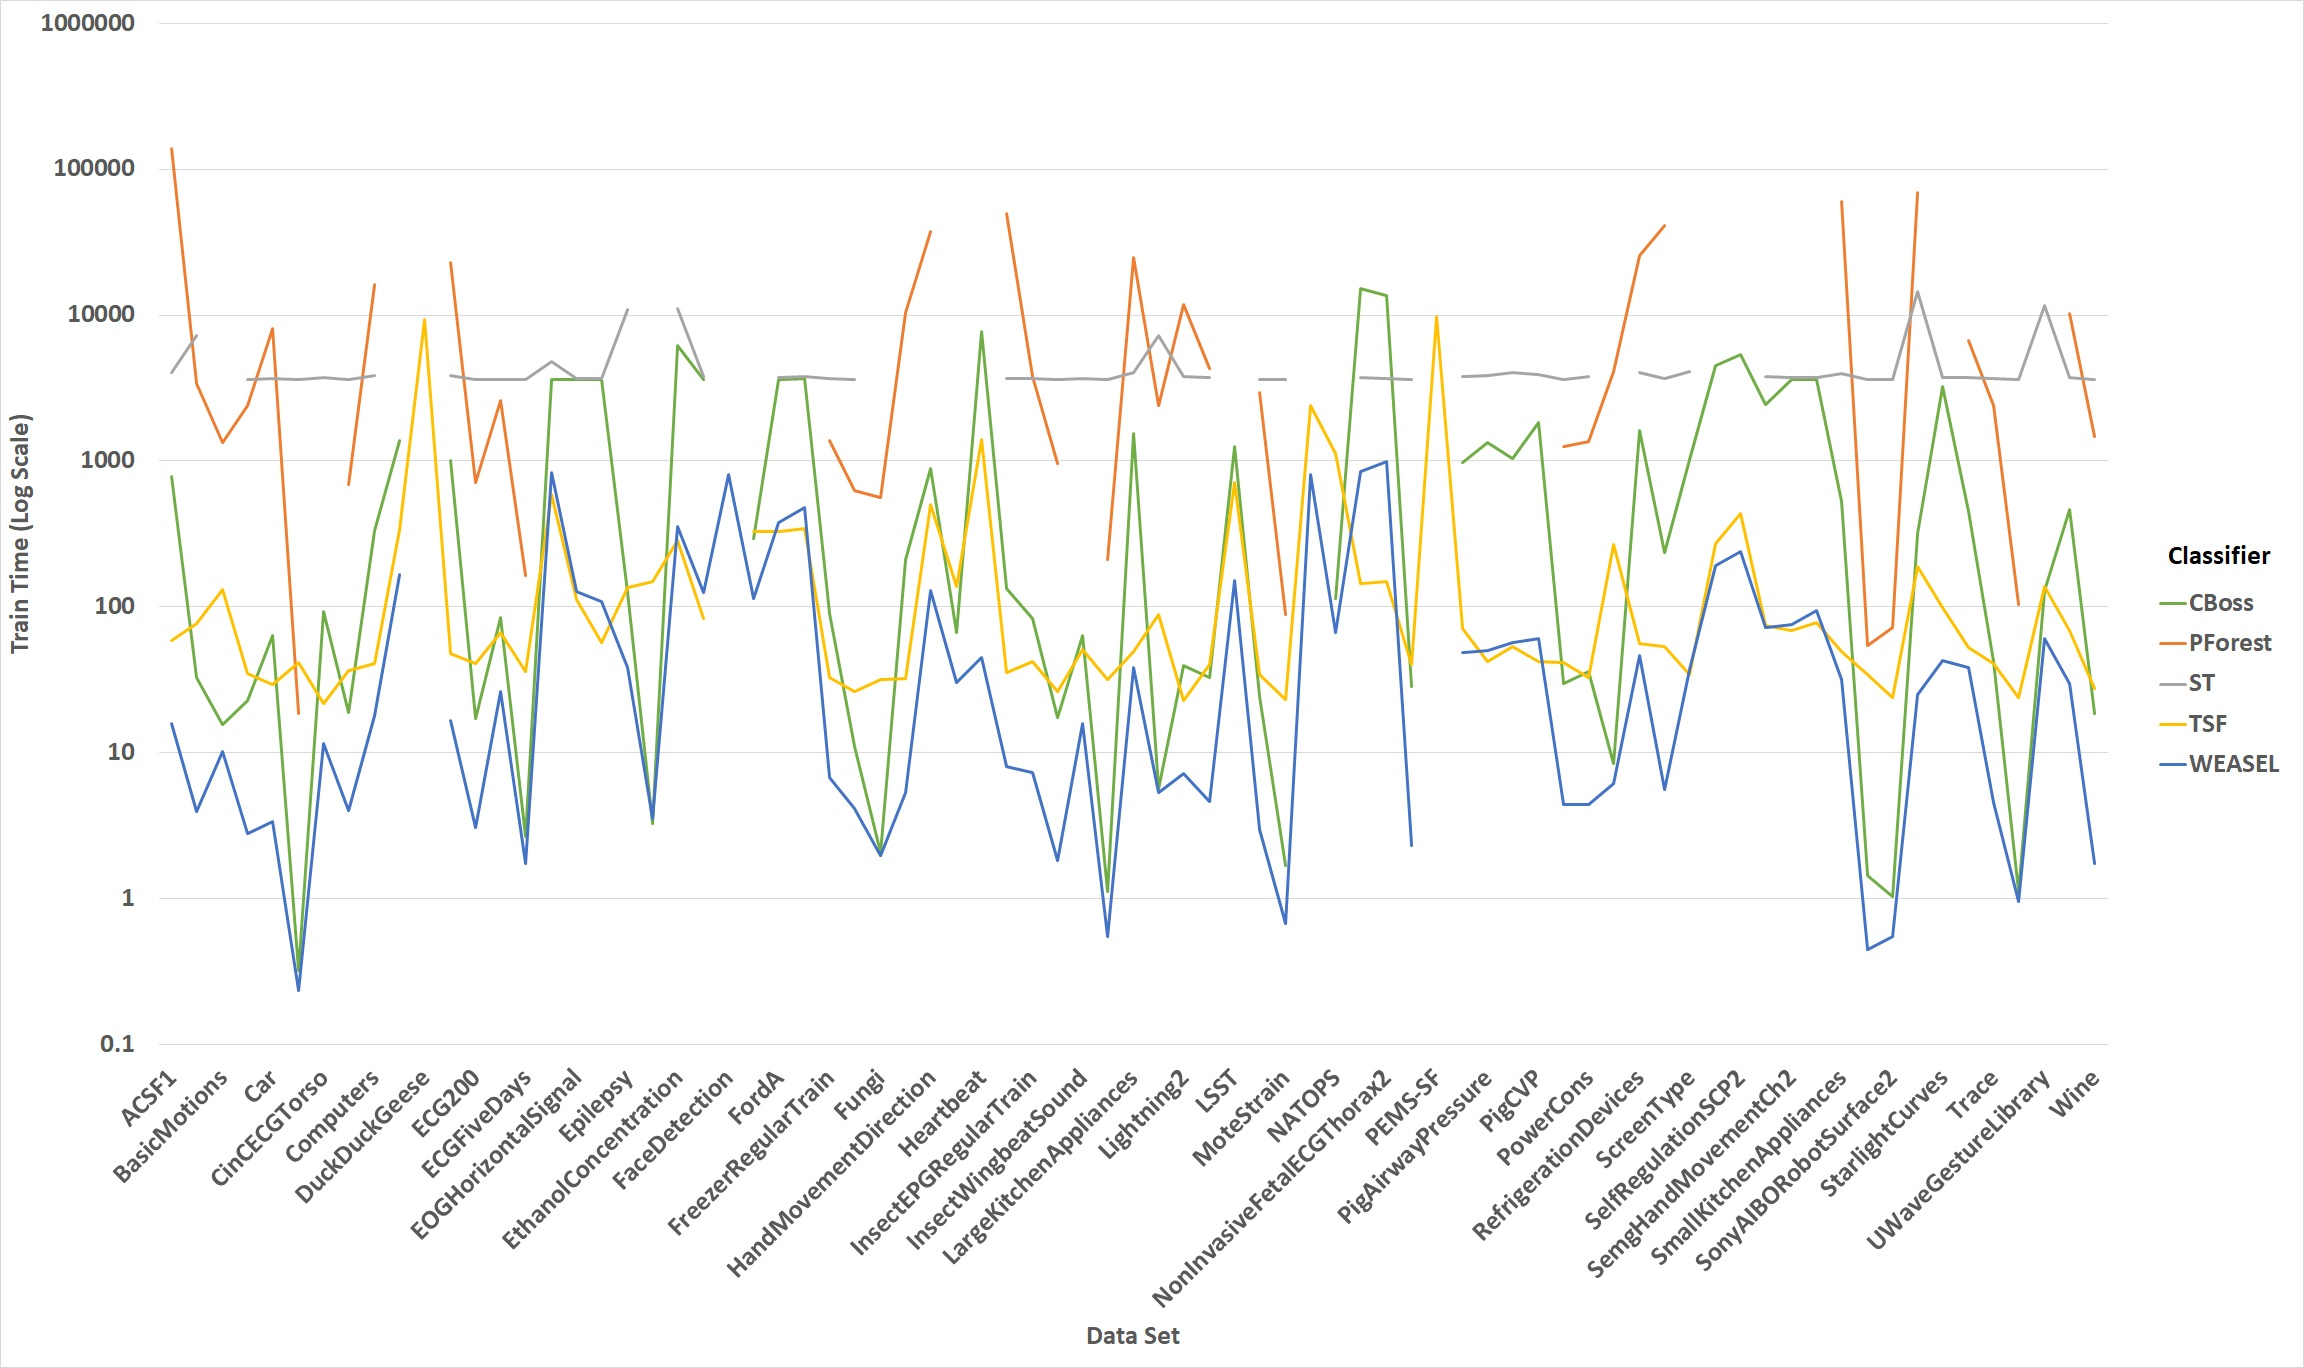
\includegraphics[width=\textwidth]{./Chapters/06 Results/Duration_30pct.jpg}
    \caption{Train Time (CPU Time in Log Scale) for all 5 classifiers for 30\% chunk}
    \label{fig:Duration30Line}
  \end{figure}
  
  \begin{figure} [!htb]
    \centering
    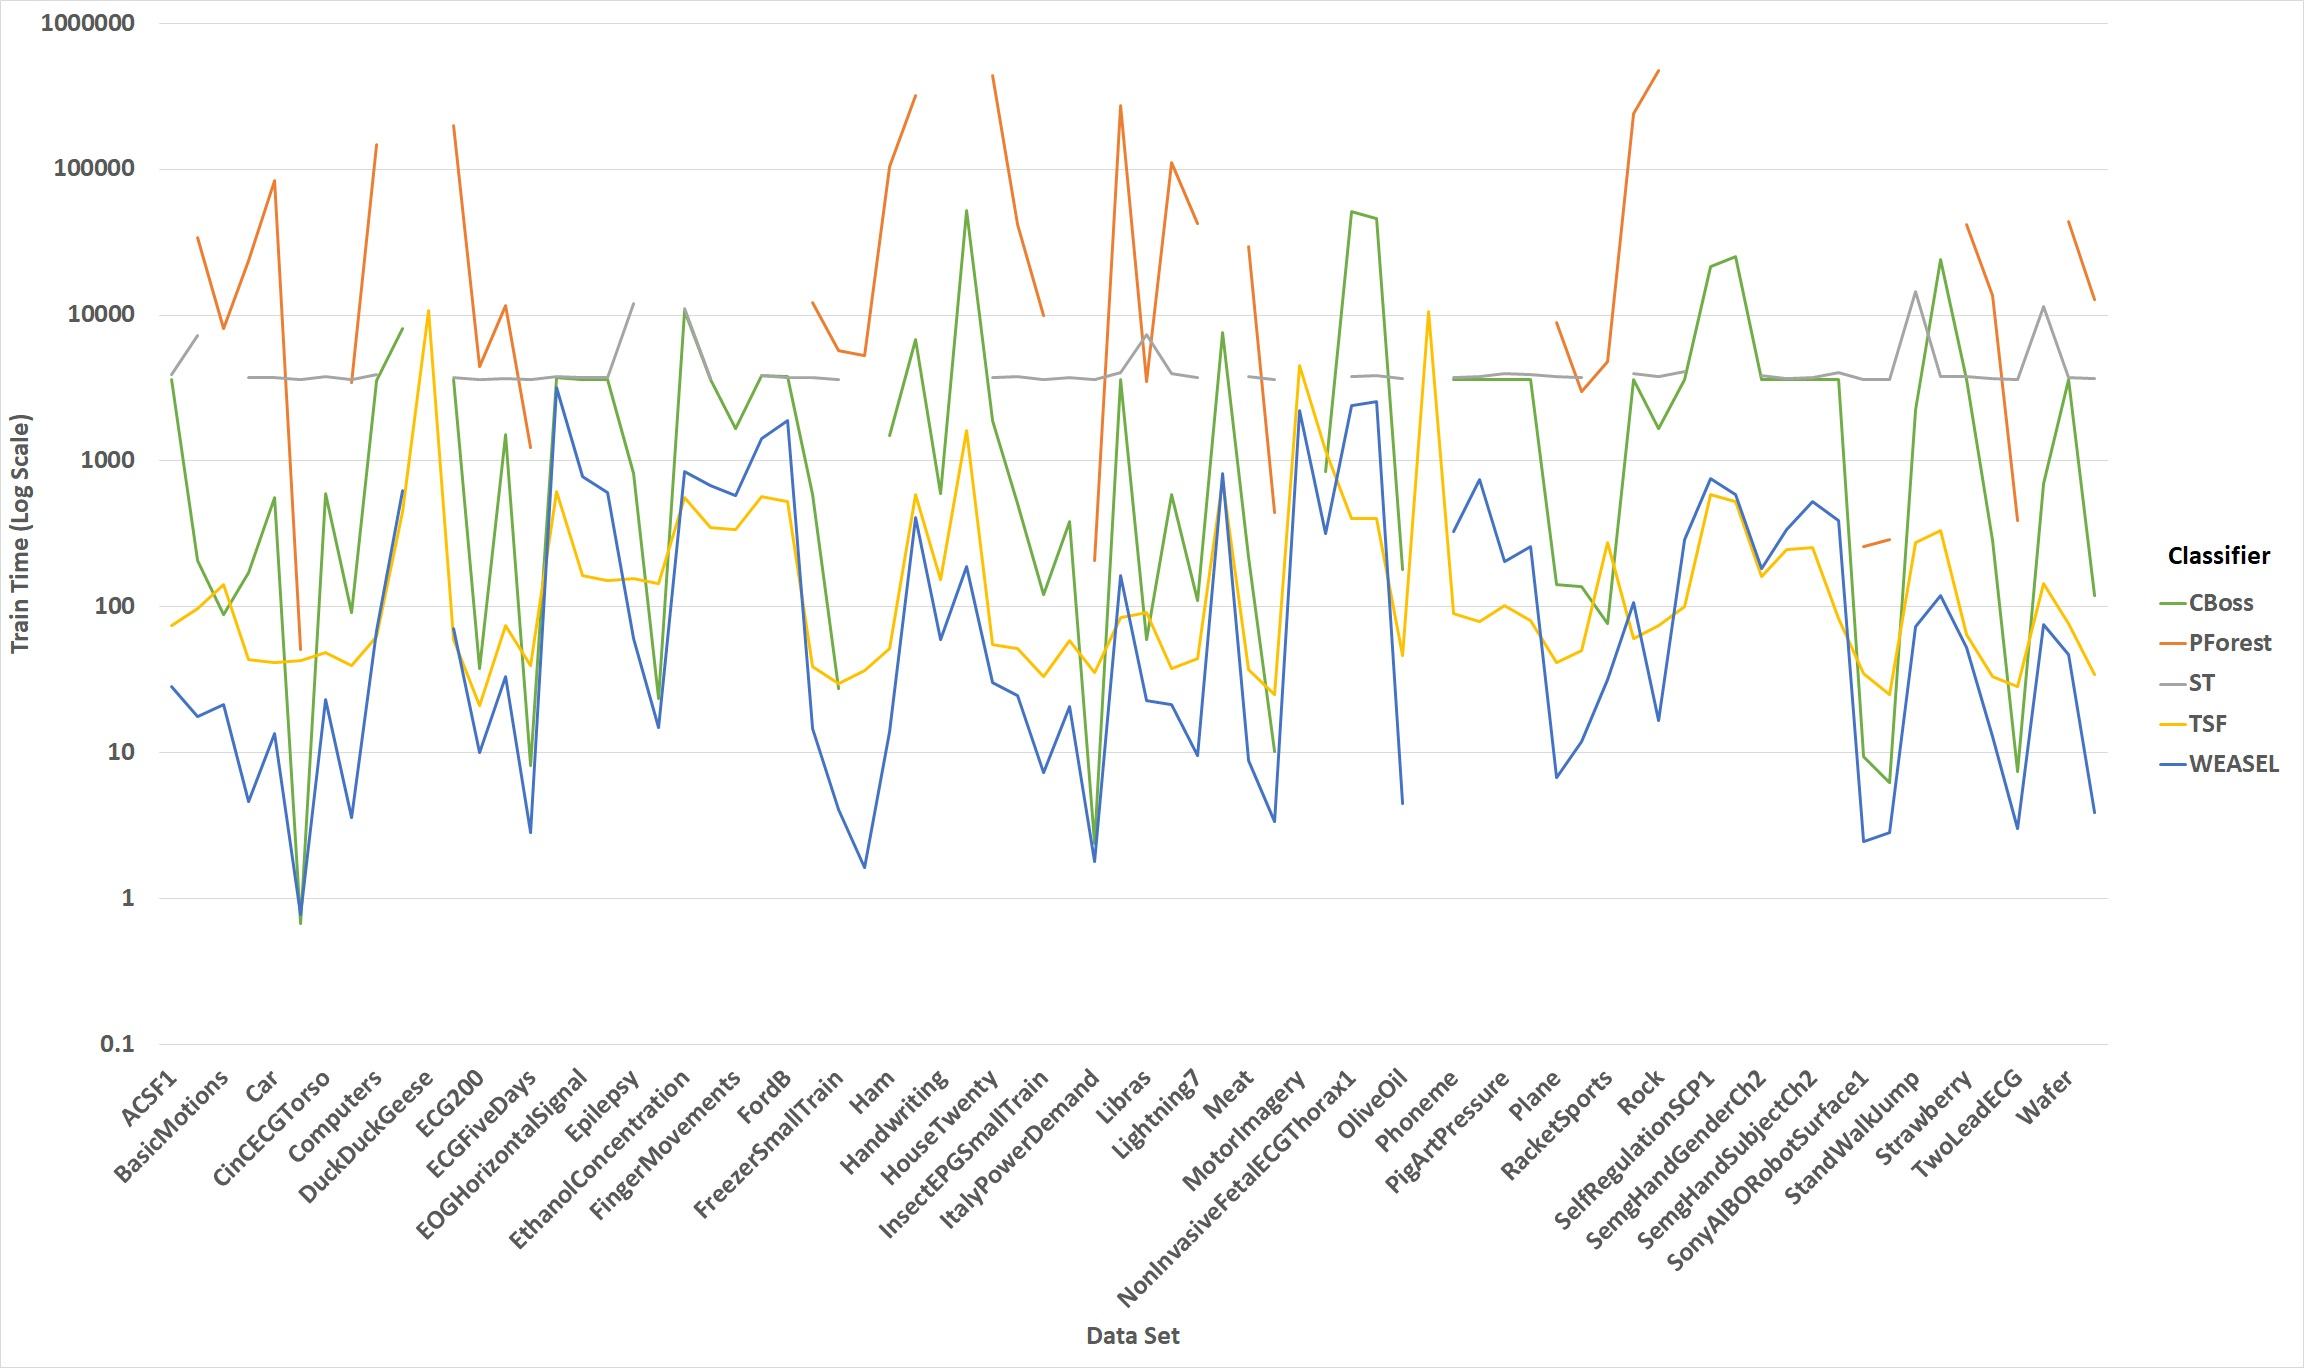
\includegraphics[width=\textwidth]{./Chapters/06 Results/Duration_100pct.jpg}
    \caption{Train Time (CPU Time in Log Scale) for all 5 classifiers for 100\% chunk}
    \label{fig:Duration100Line}
  \end{figure}
%%%%%%%%%%%%%
  %length
  %%%%%%%%%%%%%
  \begin{figure} [!htb]
    \centering
    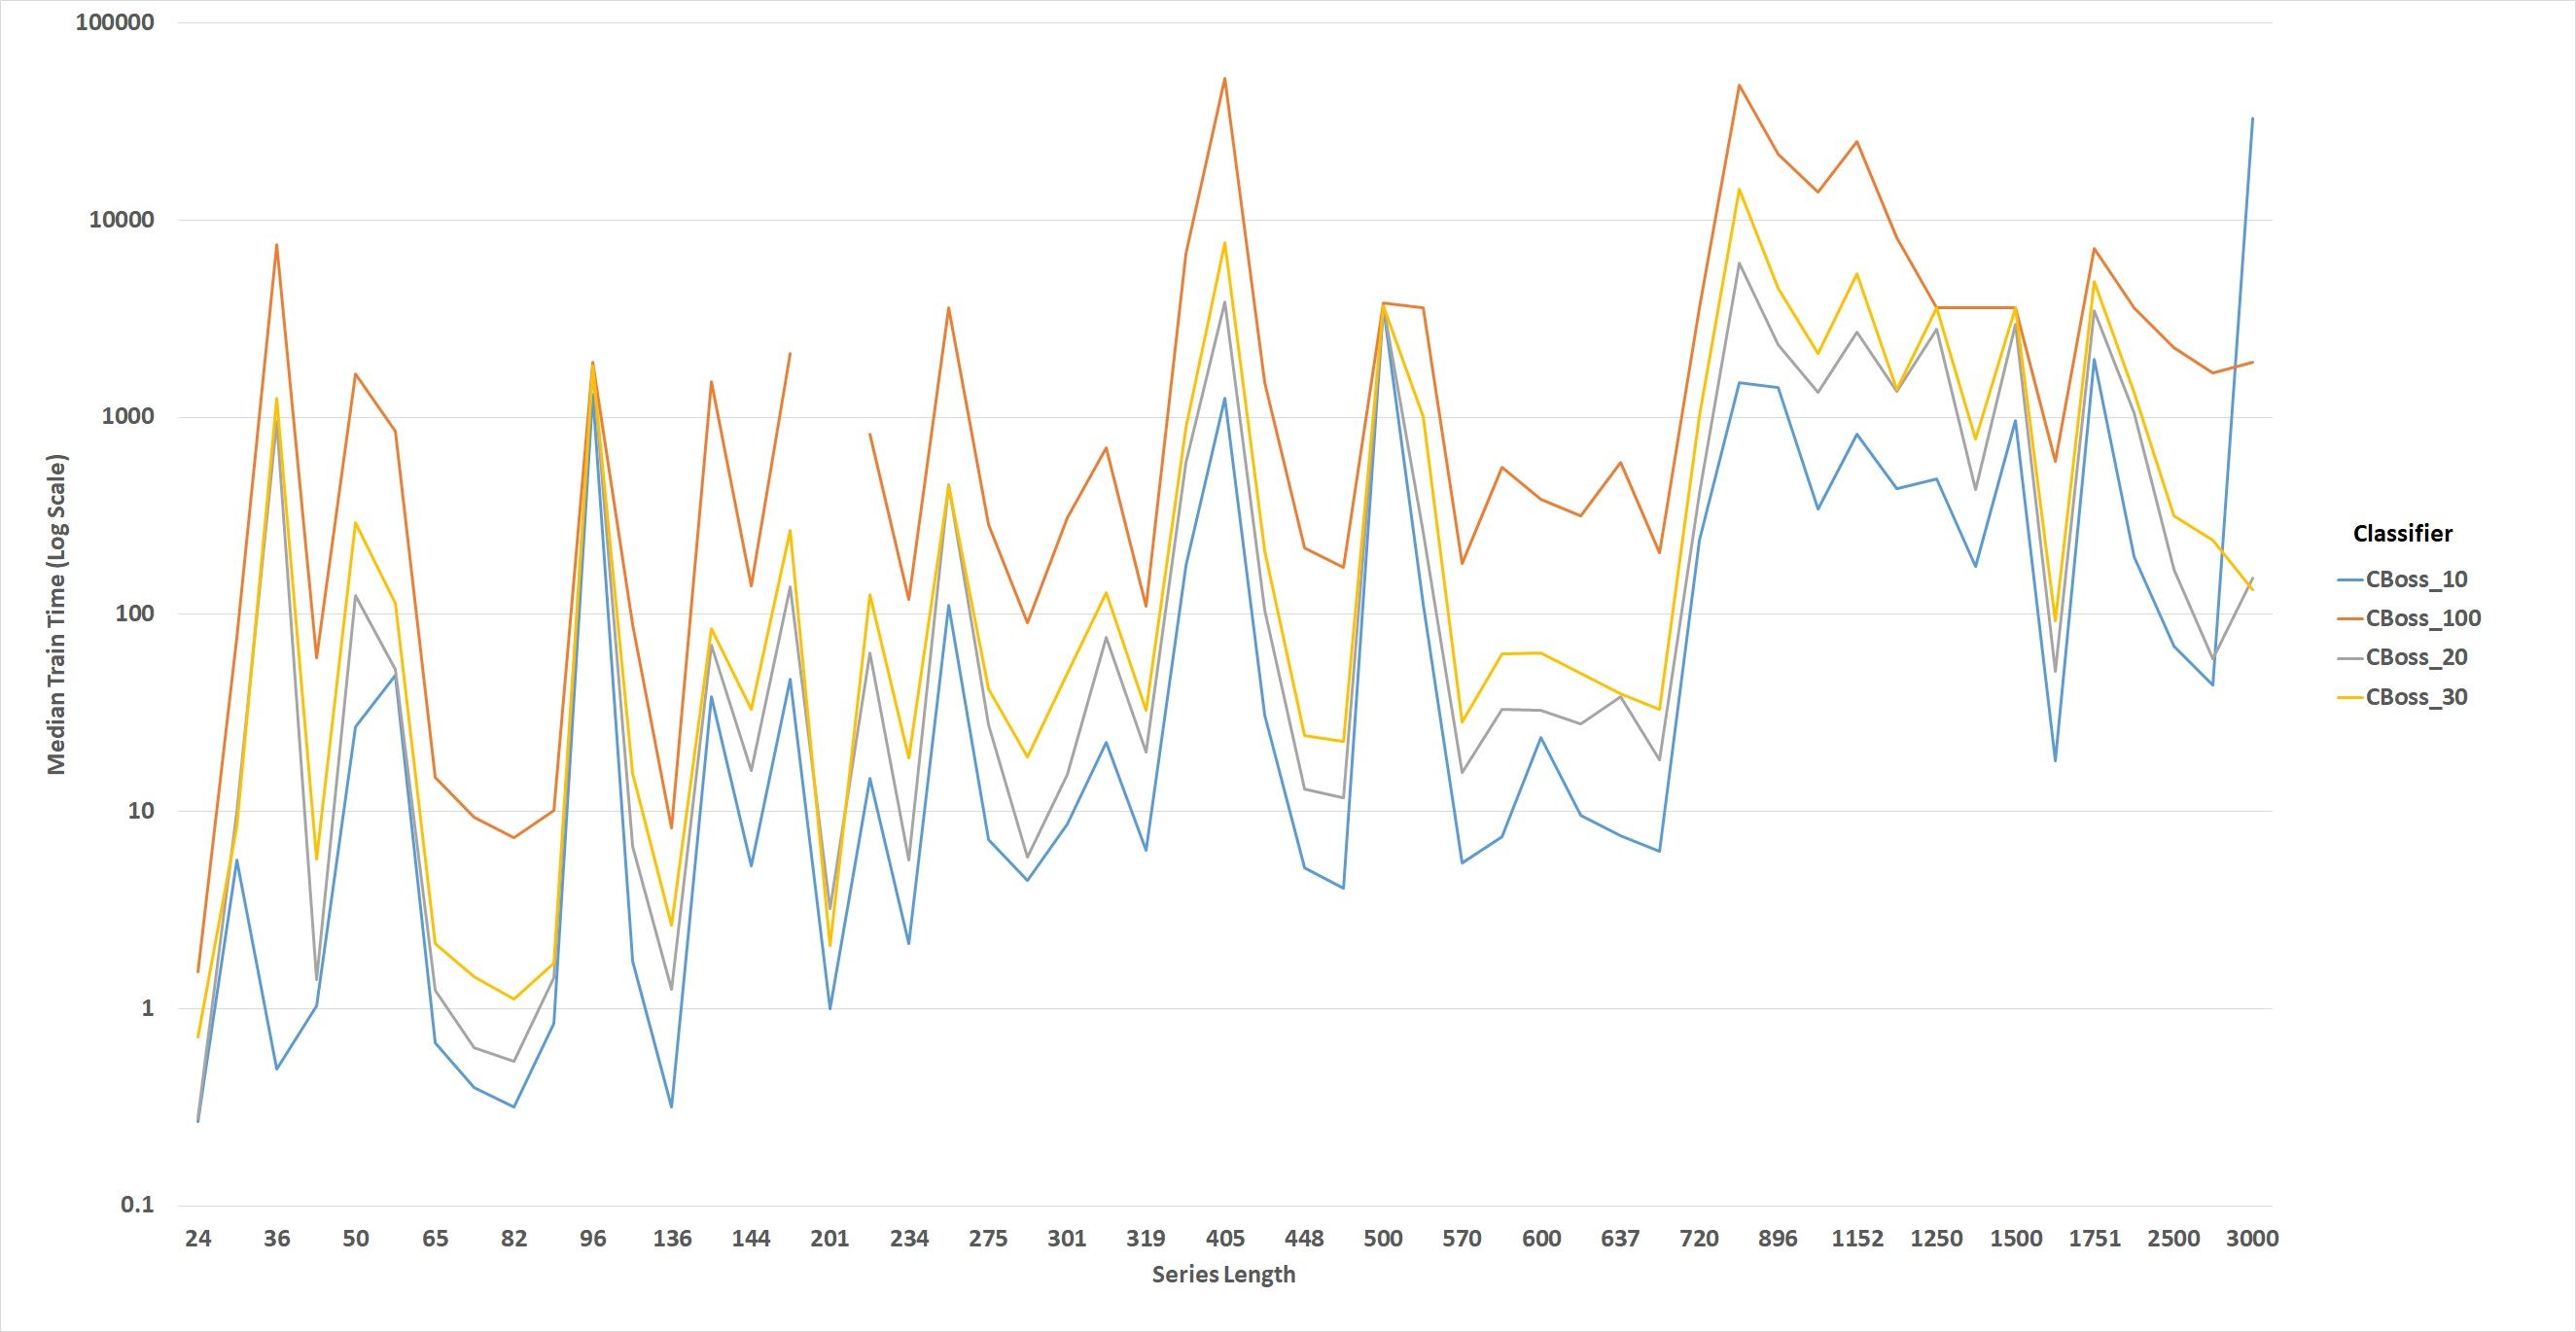
\includegraphics[width=\textwidth]{./Chapters/06 Results/Duration_cboss_length.jpg}
    \caption{Train Time (CPU Time in Log Scale) for CBOss per series length}
  \end{figure}
  
  \begin{figure} [!htb]
    \centering
    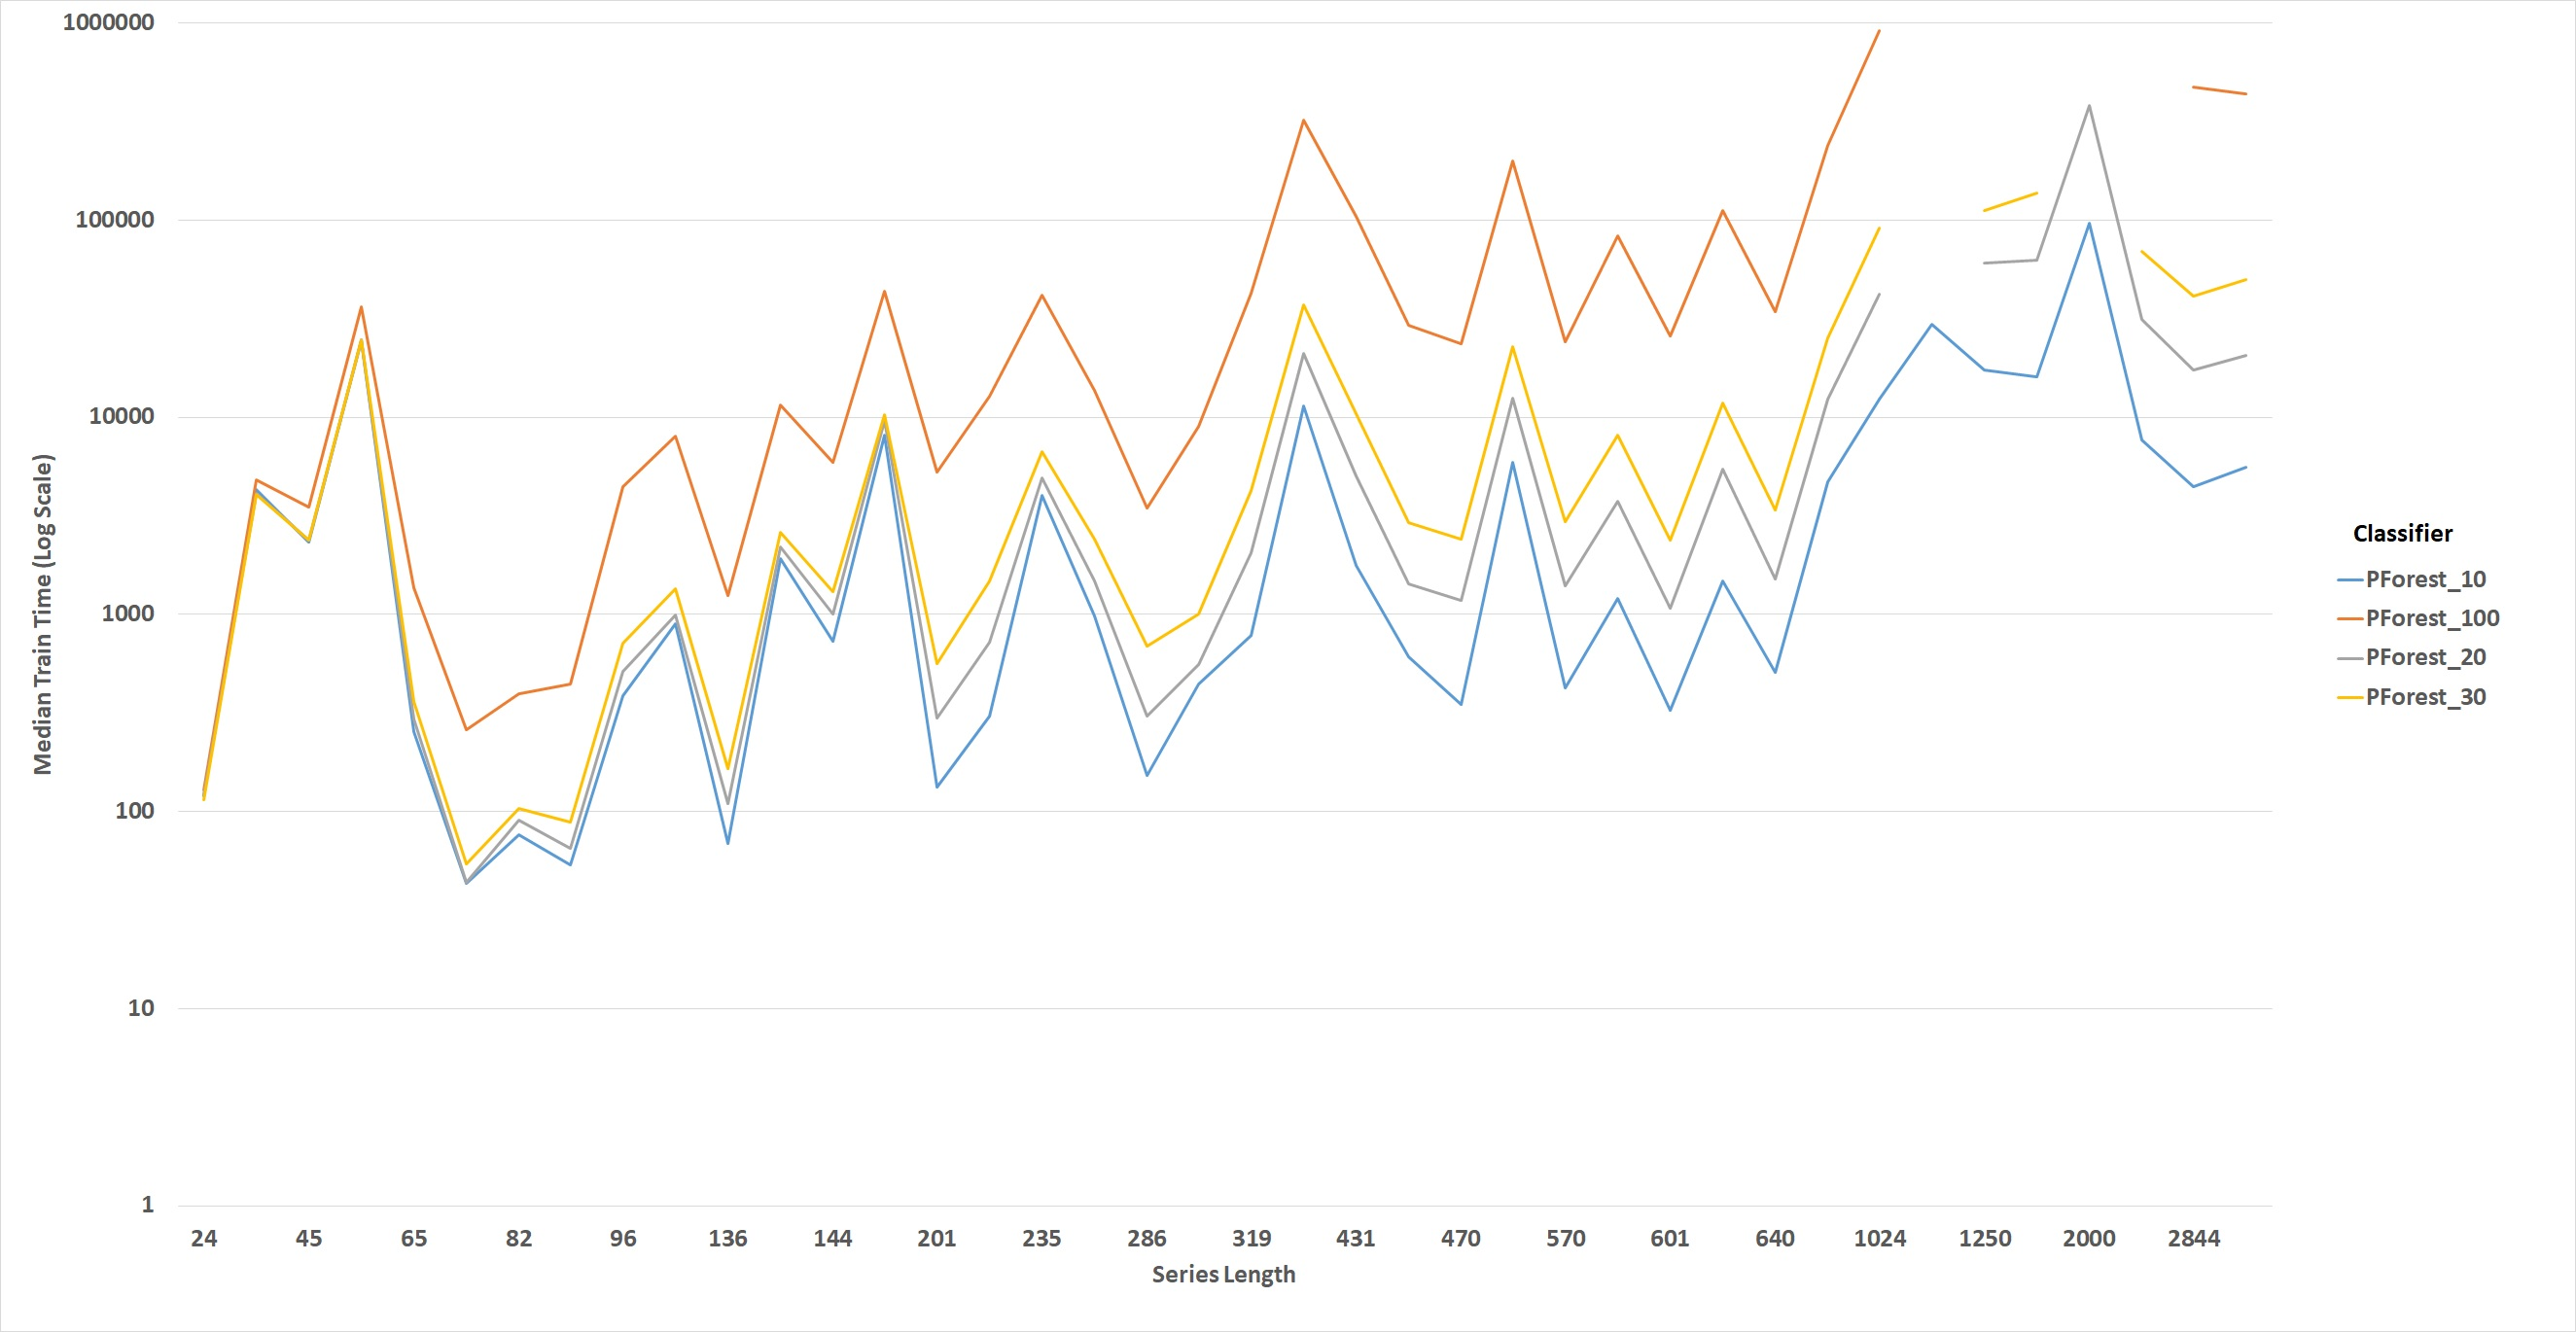
\includegraphics[width=\textwidth]{./Chapters/06 Results/Duration_pforest_length.jpg}
    \caption{Train Time (CPU Time in Log Scale) for PForest per series length}
  \end{figure}
  
  \begin{figure} [!htb]
    \centering
    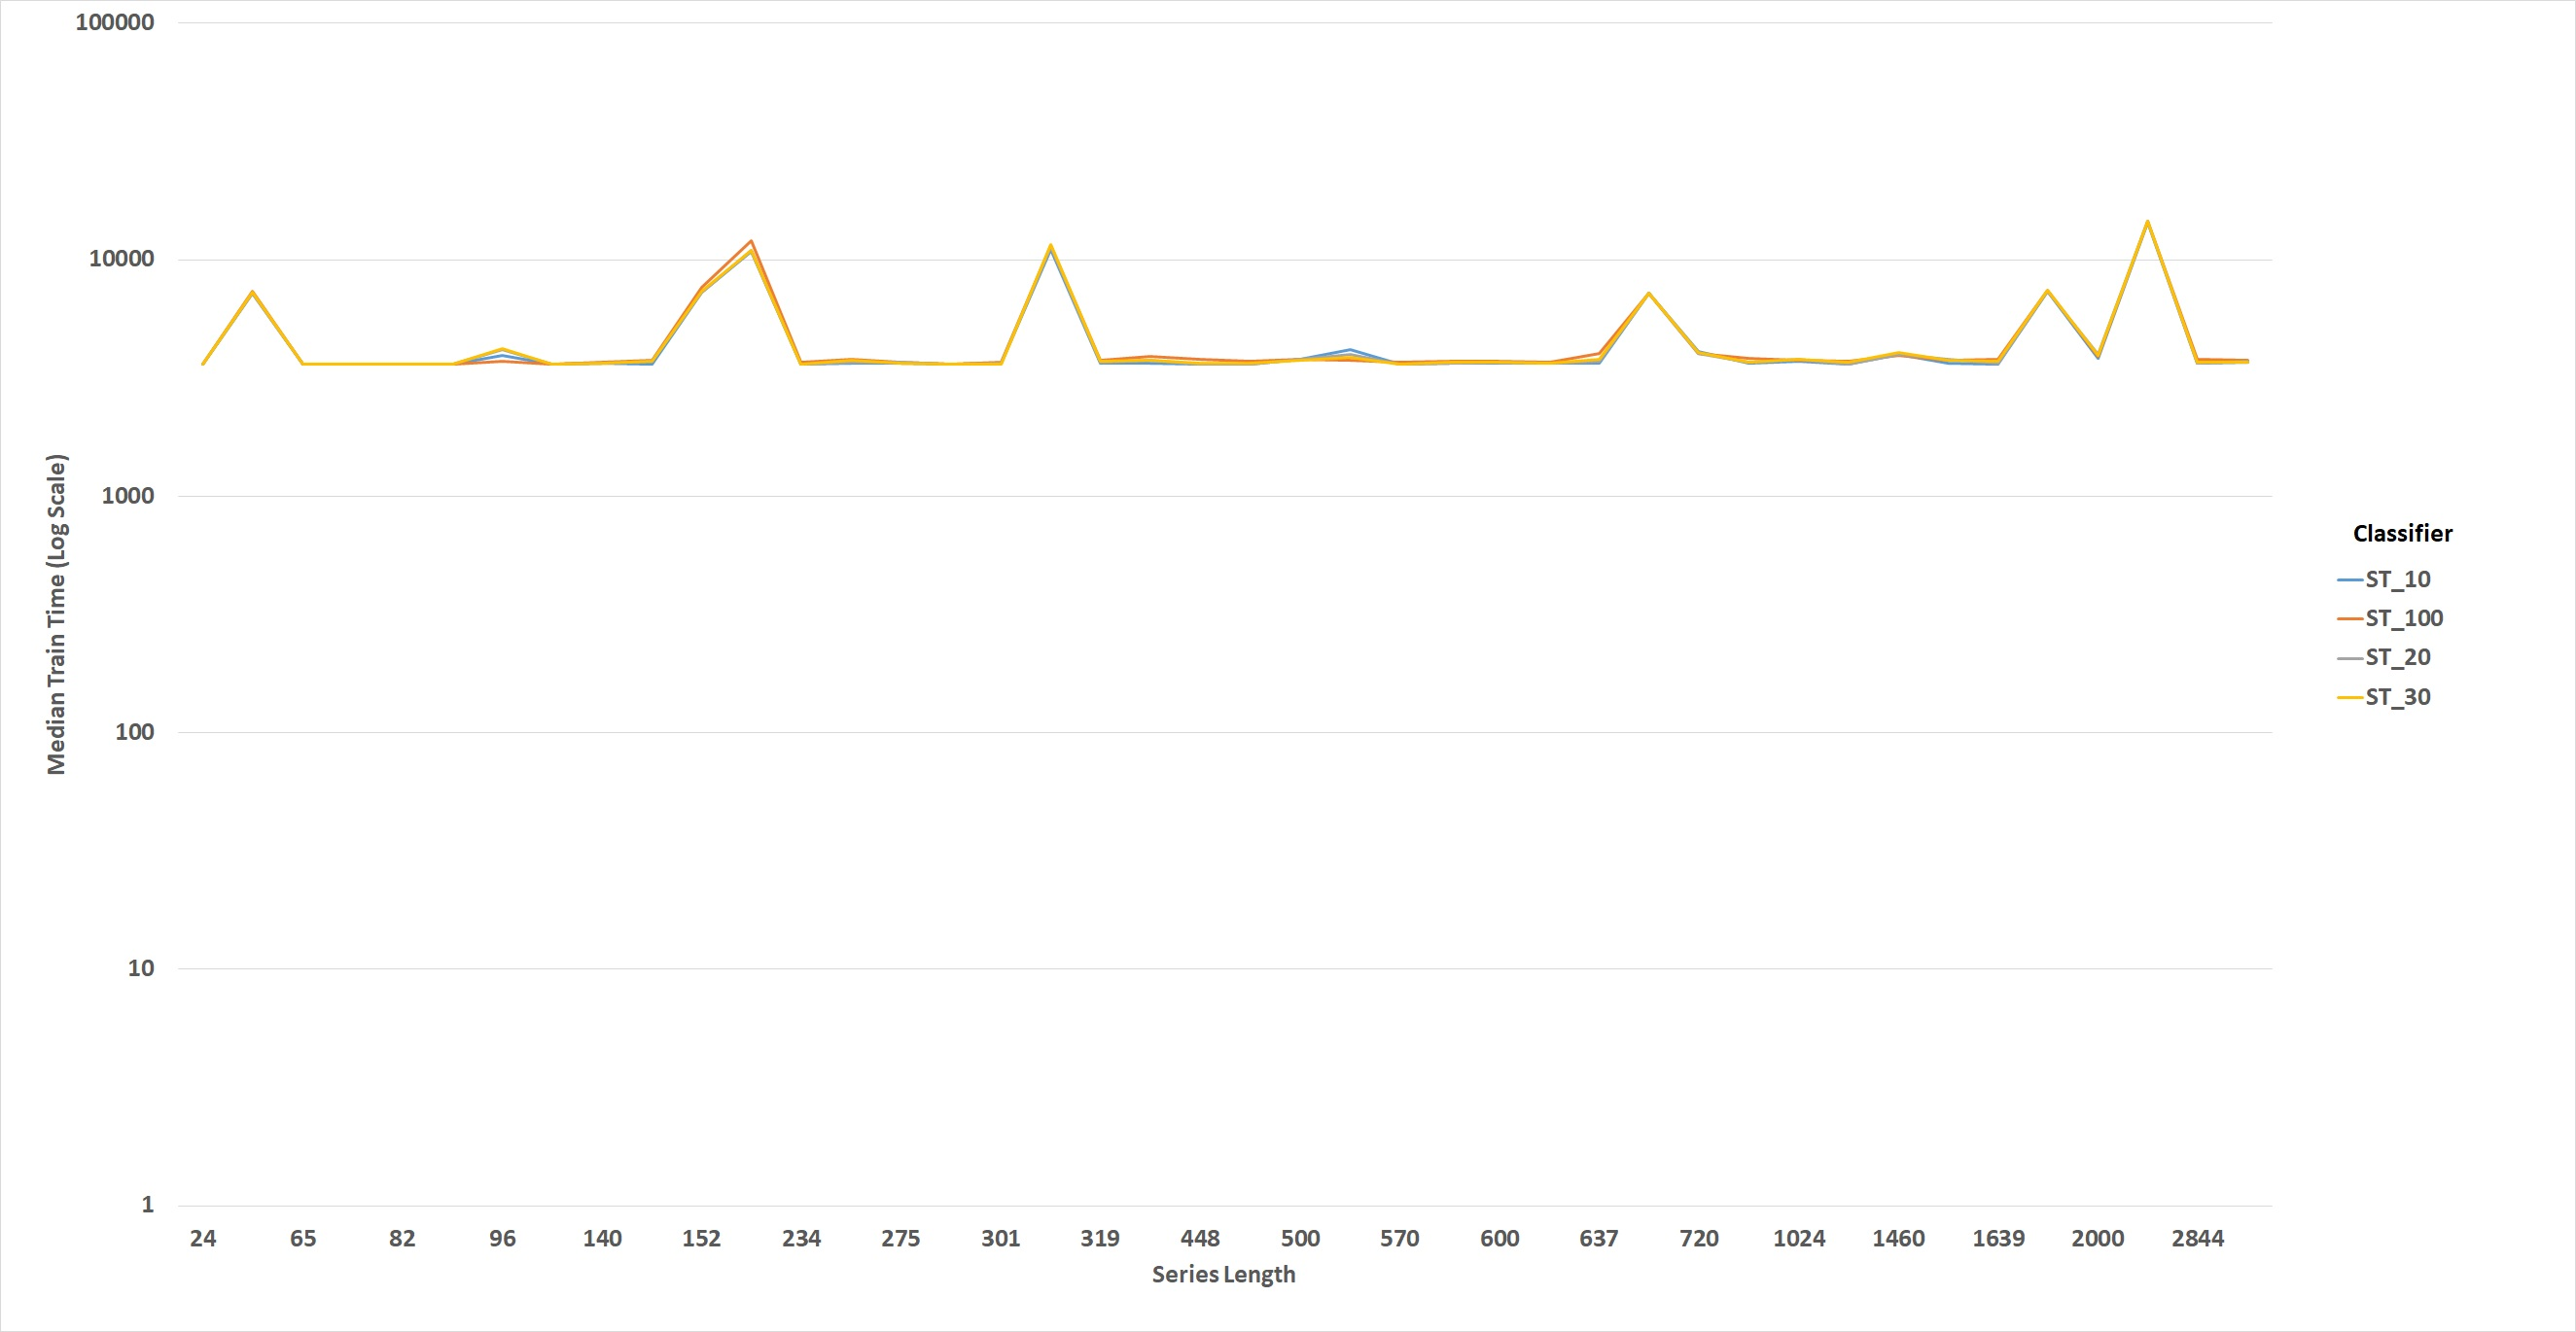
\includegraphics[width=\textwidth]{./Chapters/06 Results/Duration_st_length.jpg}
    \caption{Train Time (CPU Time in Log Scale) for ST per series length}
  \end{figure}
  
  \begin{figure} [!htb]
    \centering
    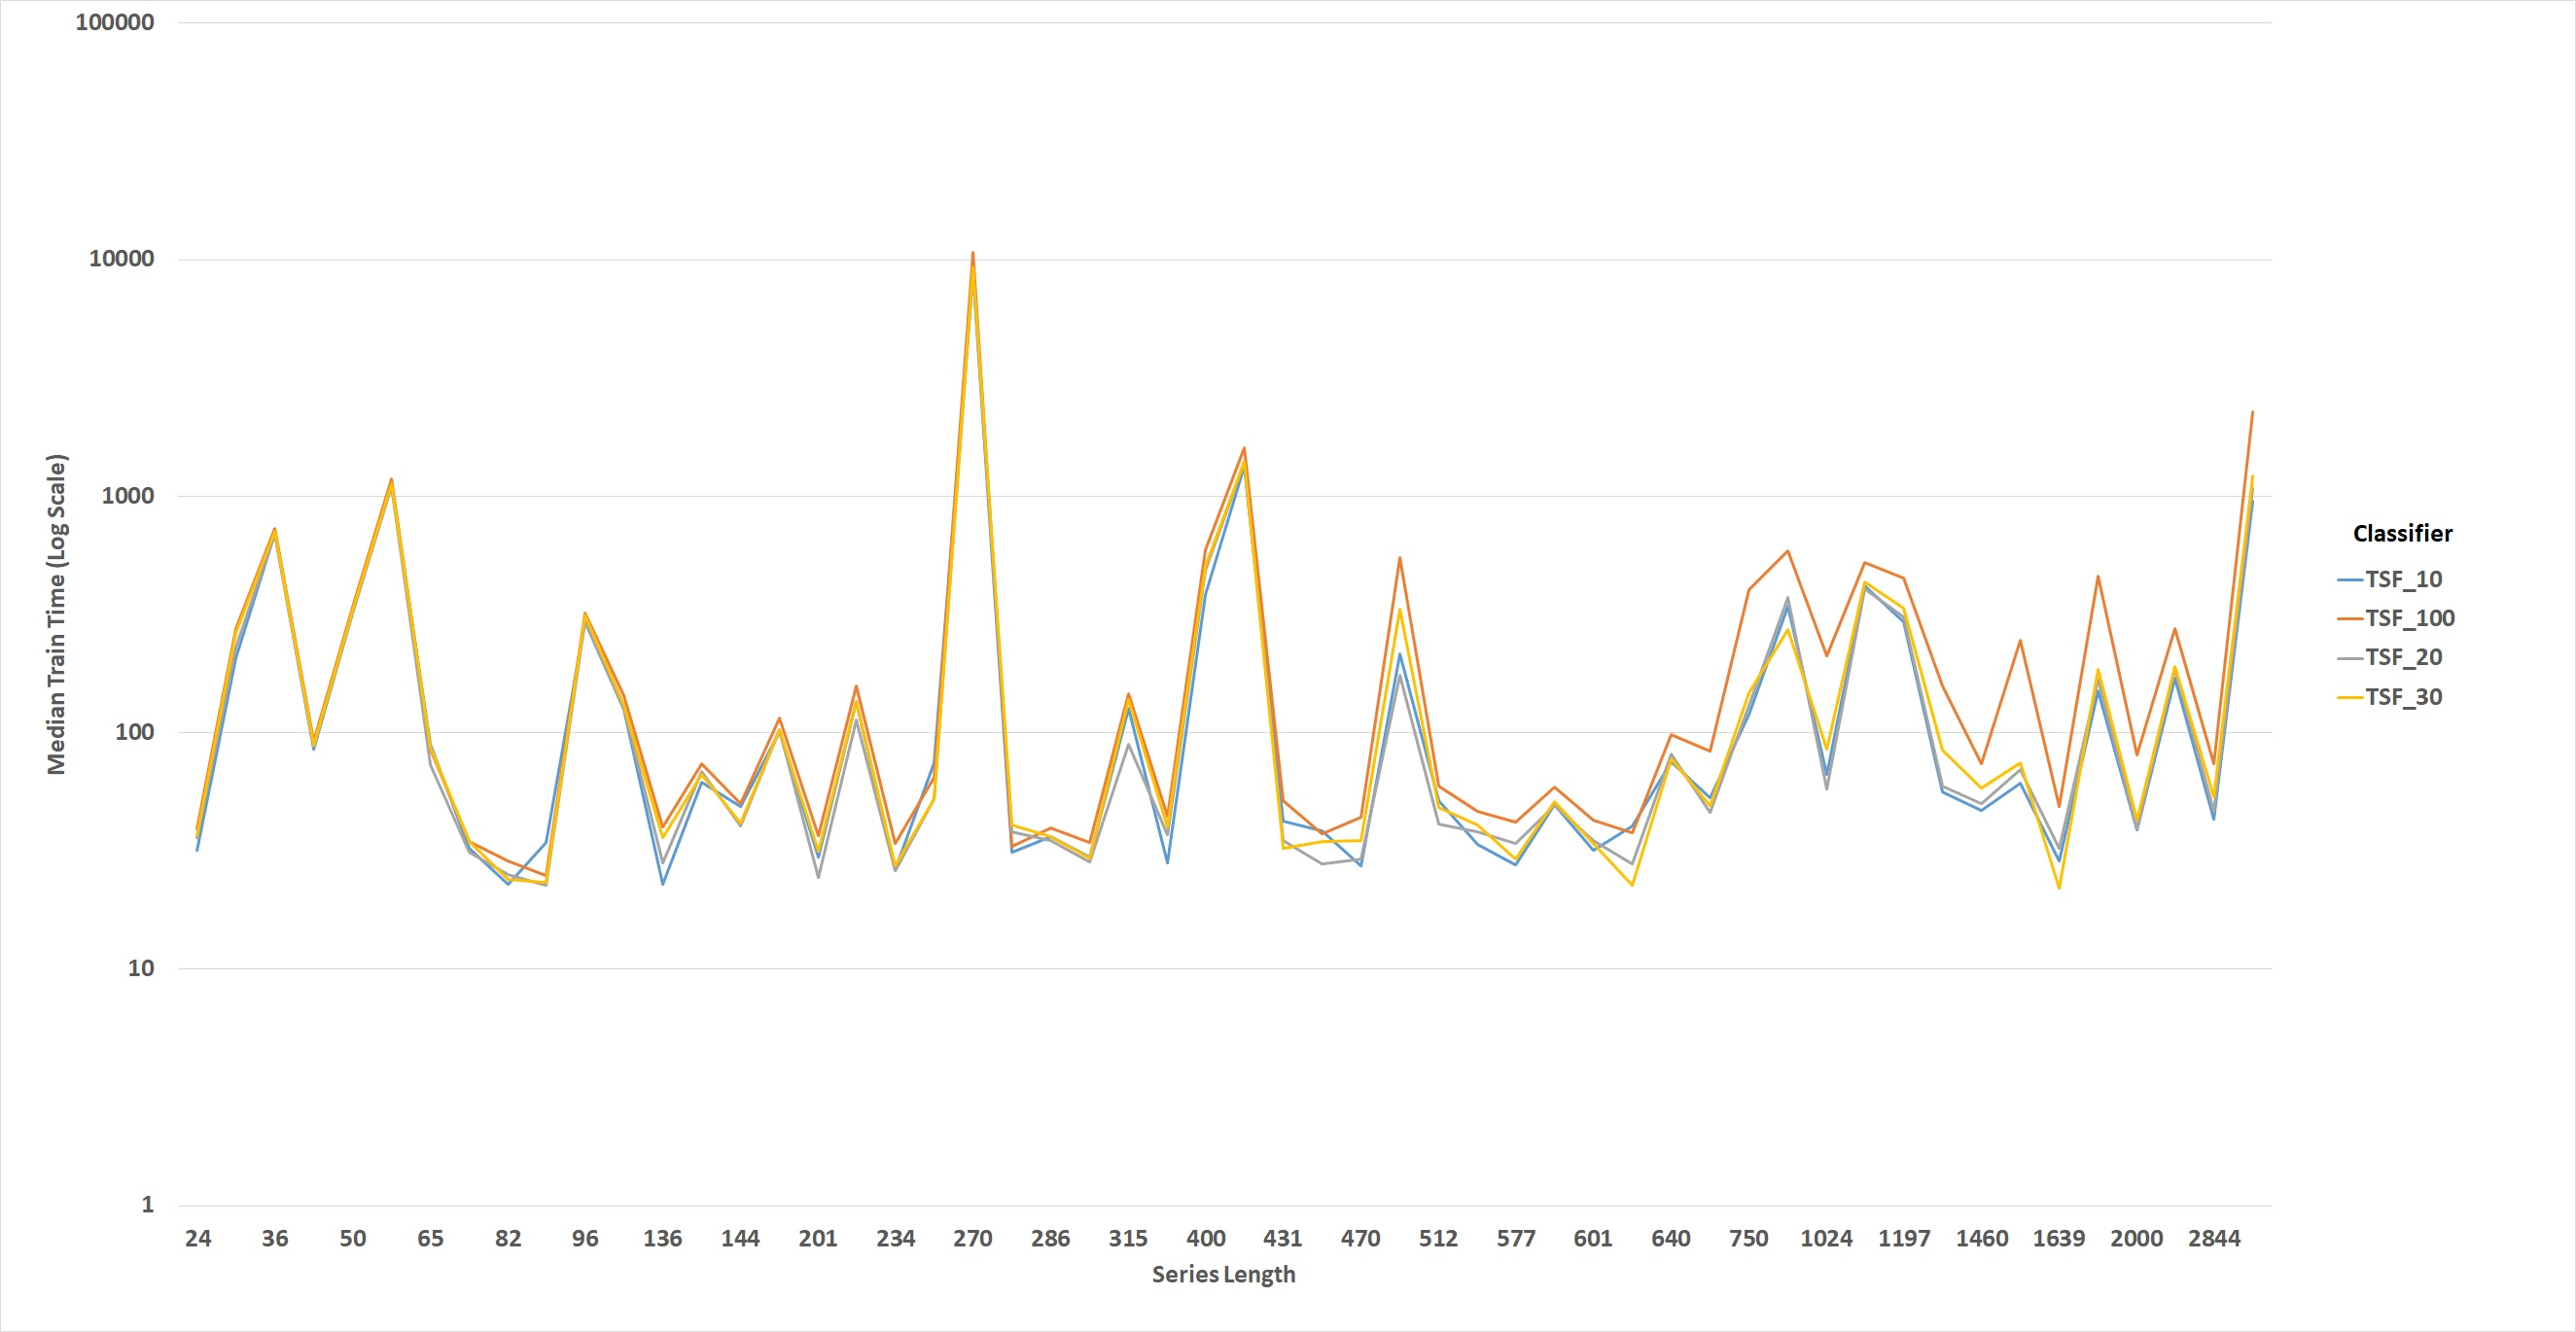
\includegraphics[width=\textwidth]{./Chapters/06 Results/Duration_tsf_length.jpg}
    \caption{Train Time (CPU Time in Log Scale) for TSF per series length}
  \end{figure}

  \begin{figure} [!htb]
    \centering
    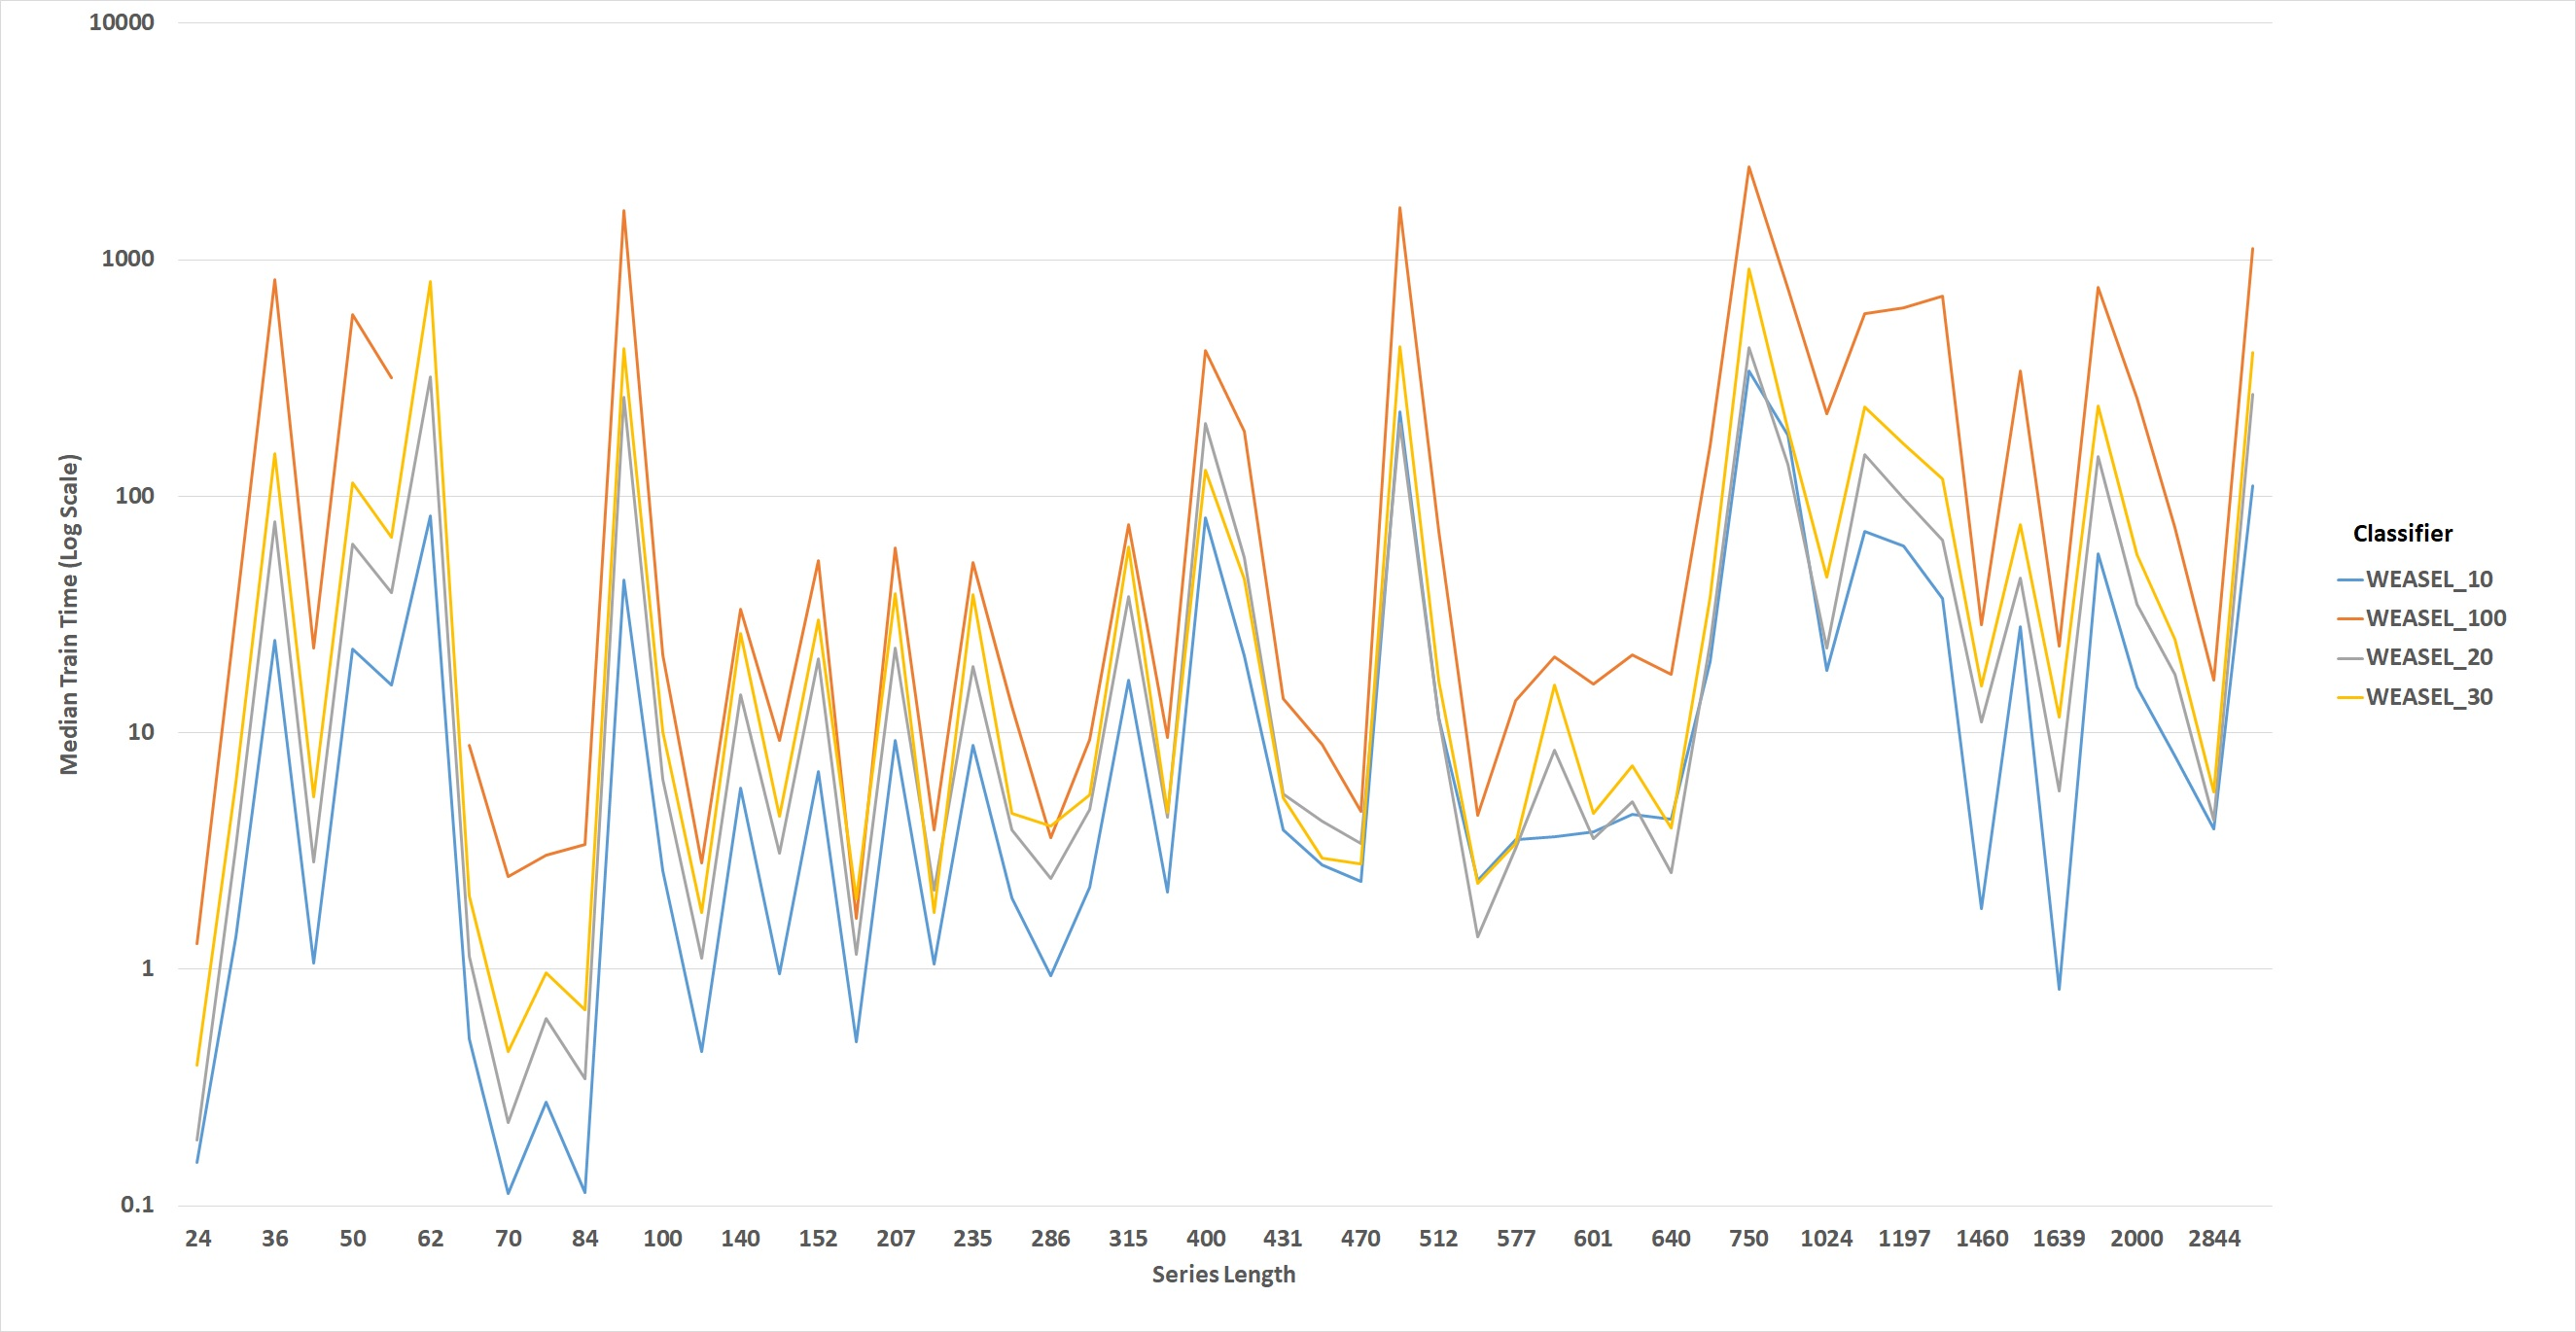
\includegraphics[width=\textwidth]{./Chapters/06 Results/Duration_weasel_length.jpg}
    \caption{Train Time (CPU Time in Log Scale) for WEASEL per series length}
  \end{figure}
%%%%%%%%%%%%%
  %train size
%%%%%%%%%%%%%
  \begin{figure} [!htb]
    \centering
    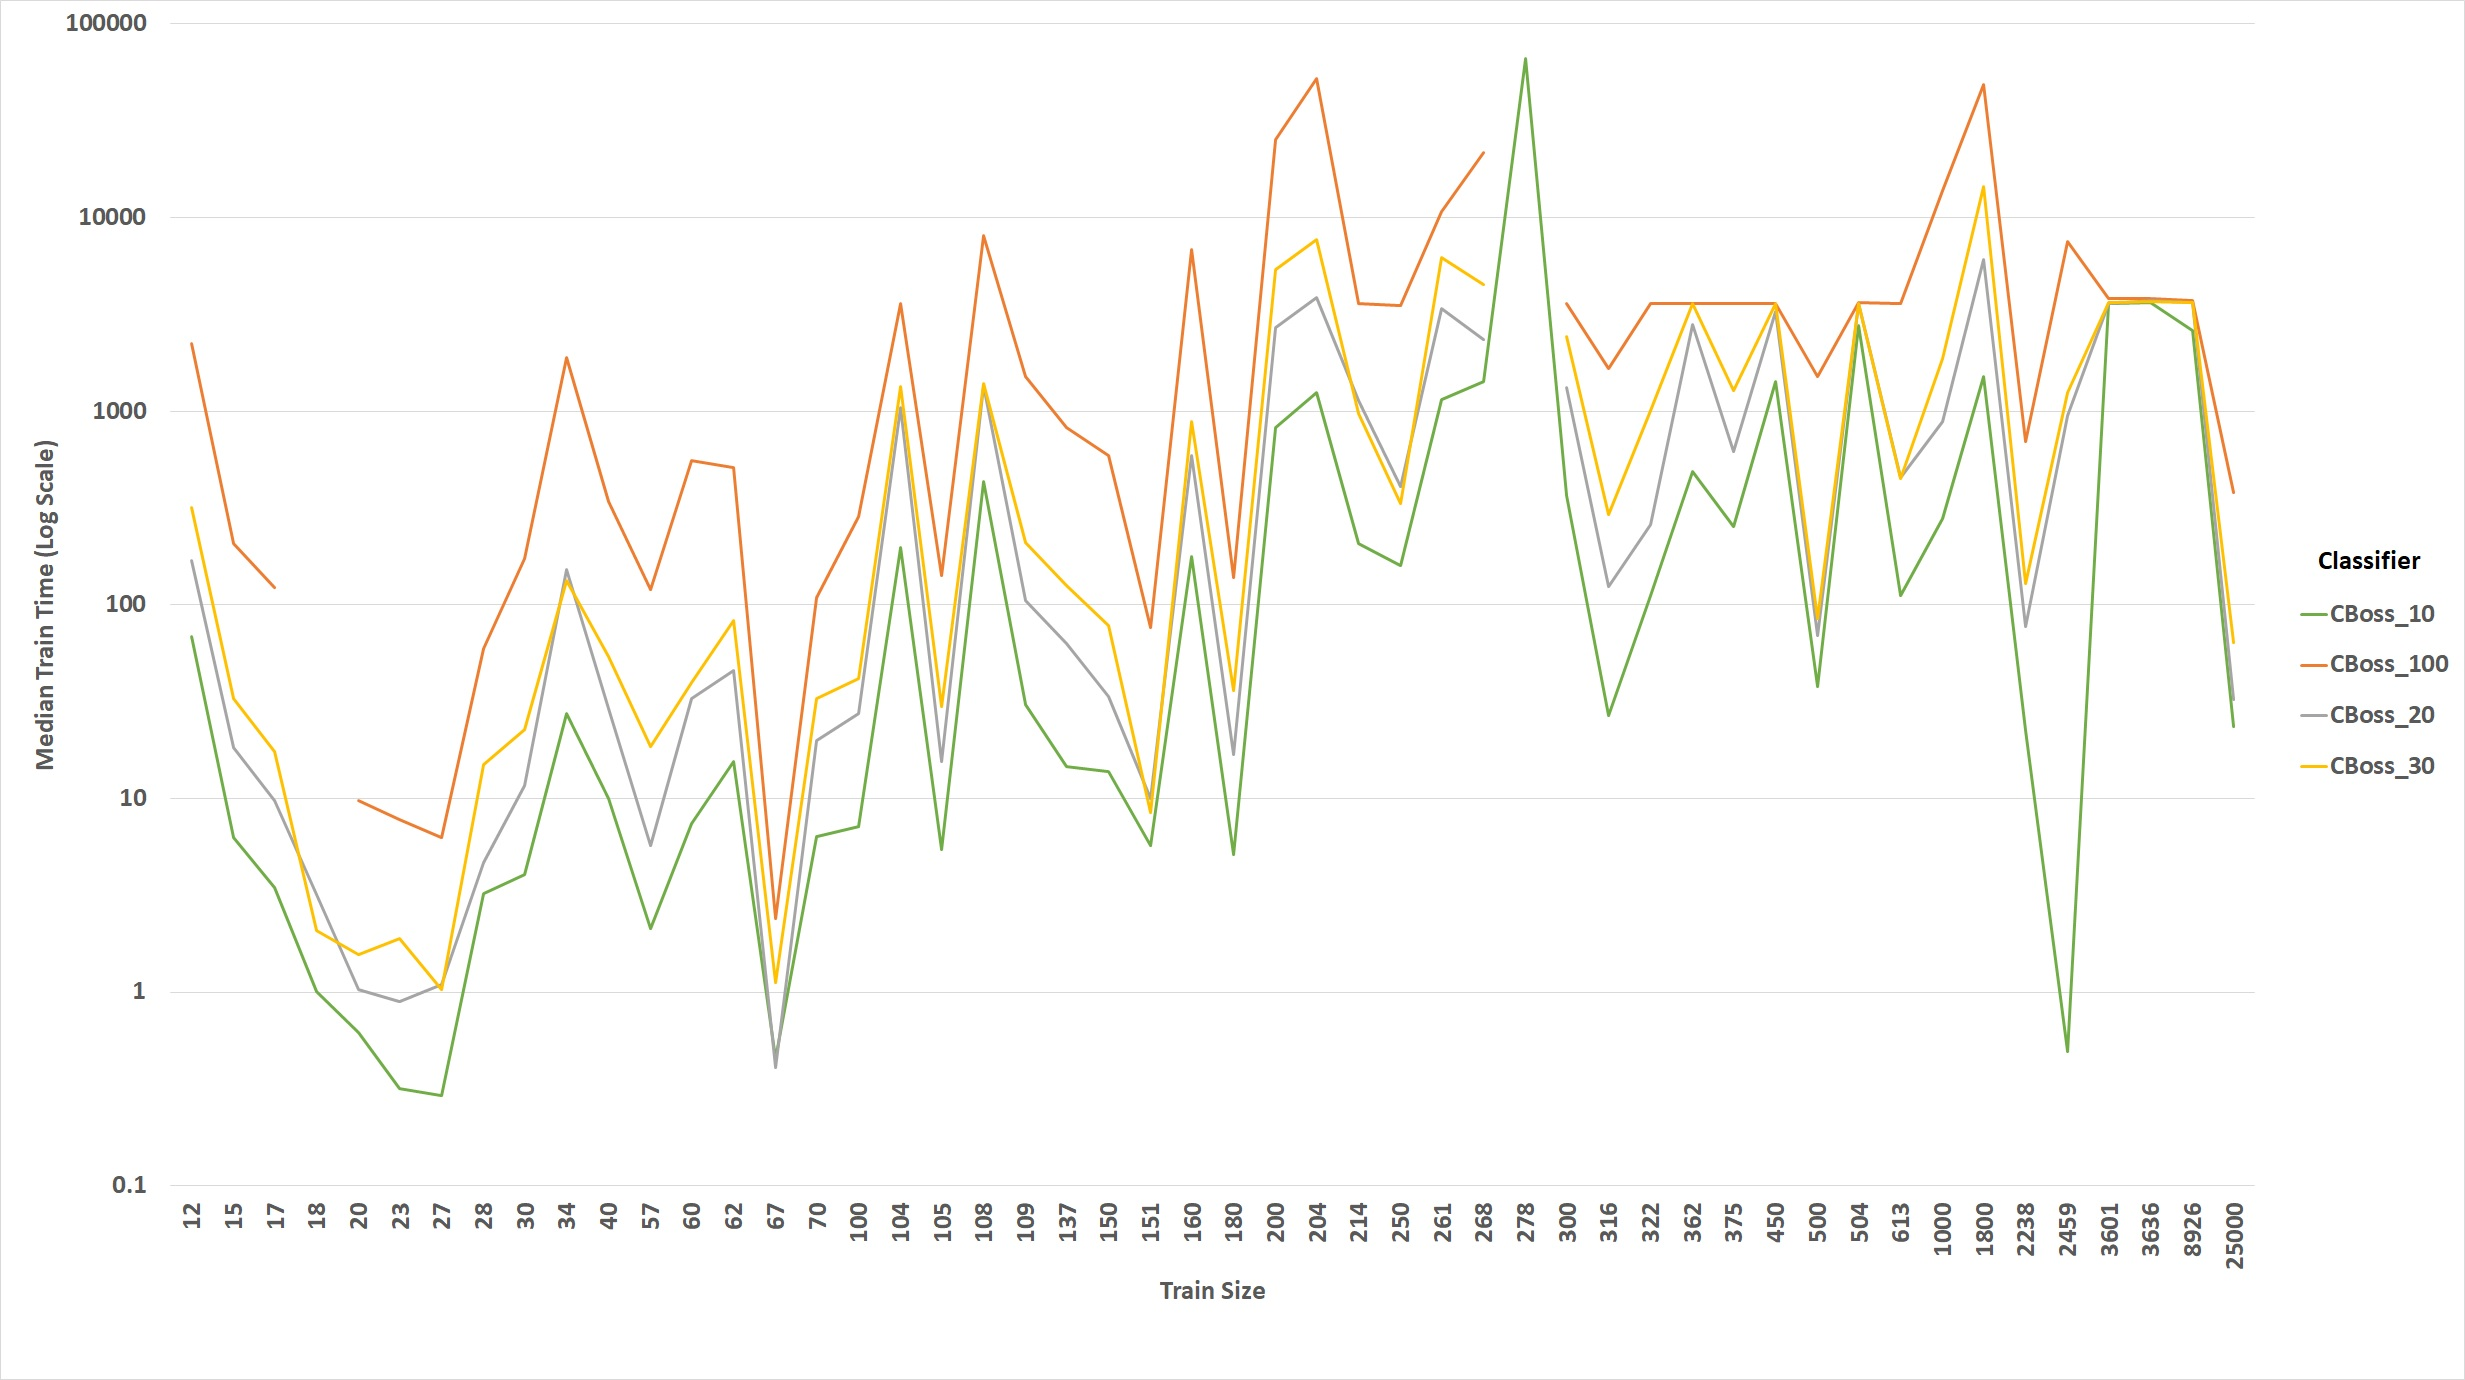
\includegraphics[width=\textwidth]{./Chapters/06 Results/Duration_cboss_train_size.jpg}
    \caption{Train Time (CPU Time in Log Scale) for CBOss per train size}
  \end{figure}
  
  \begin{figure} [!htb]
    \centering
    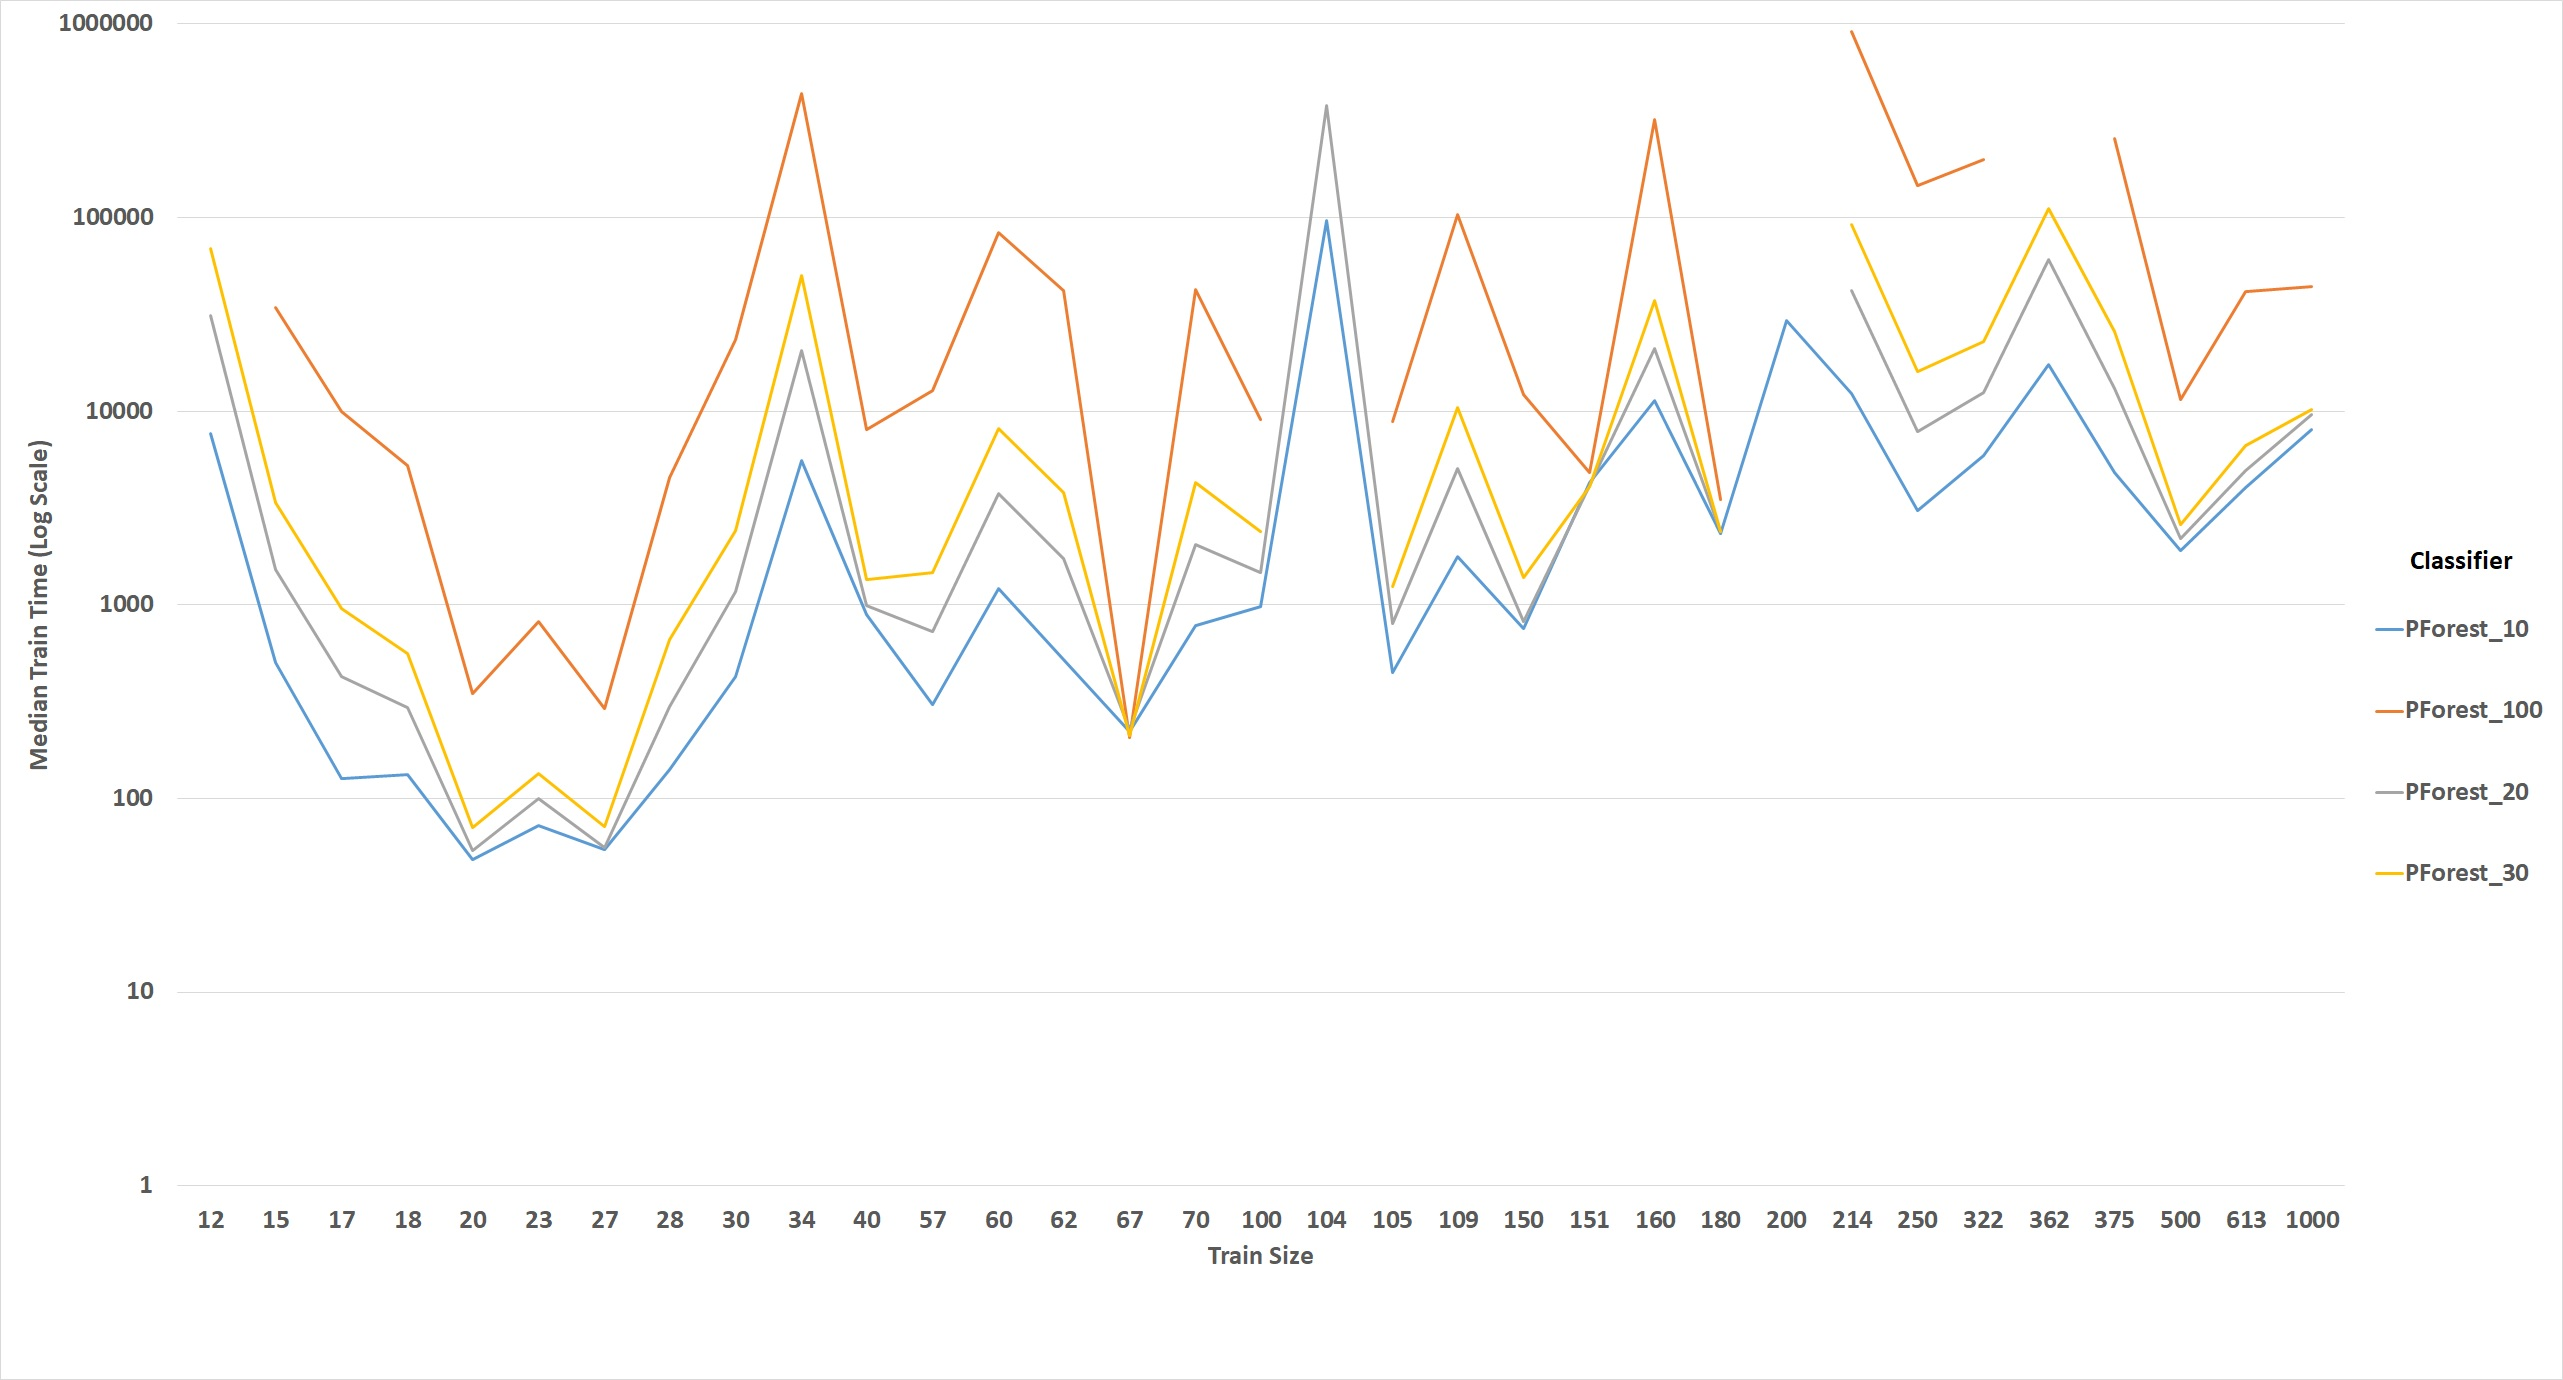
\includegraphics[width=\textwidth]{./Chapters/06 Results/Duration_pforest_train_size.jpg}
    \caption{Train Time (CPU Time in Log Scale) for PForest per train size}
  \end{figure}
  
  \begin{figure} [!htb]
    \centering
    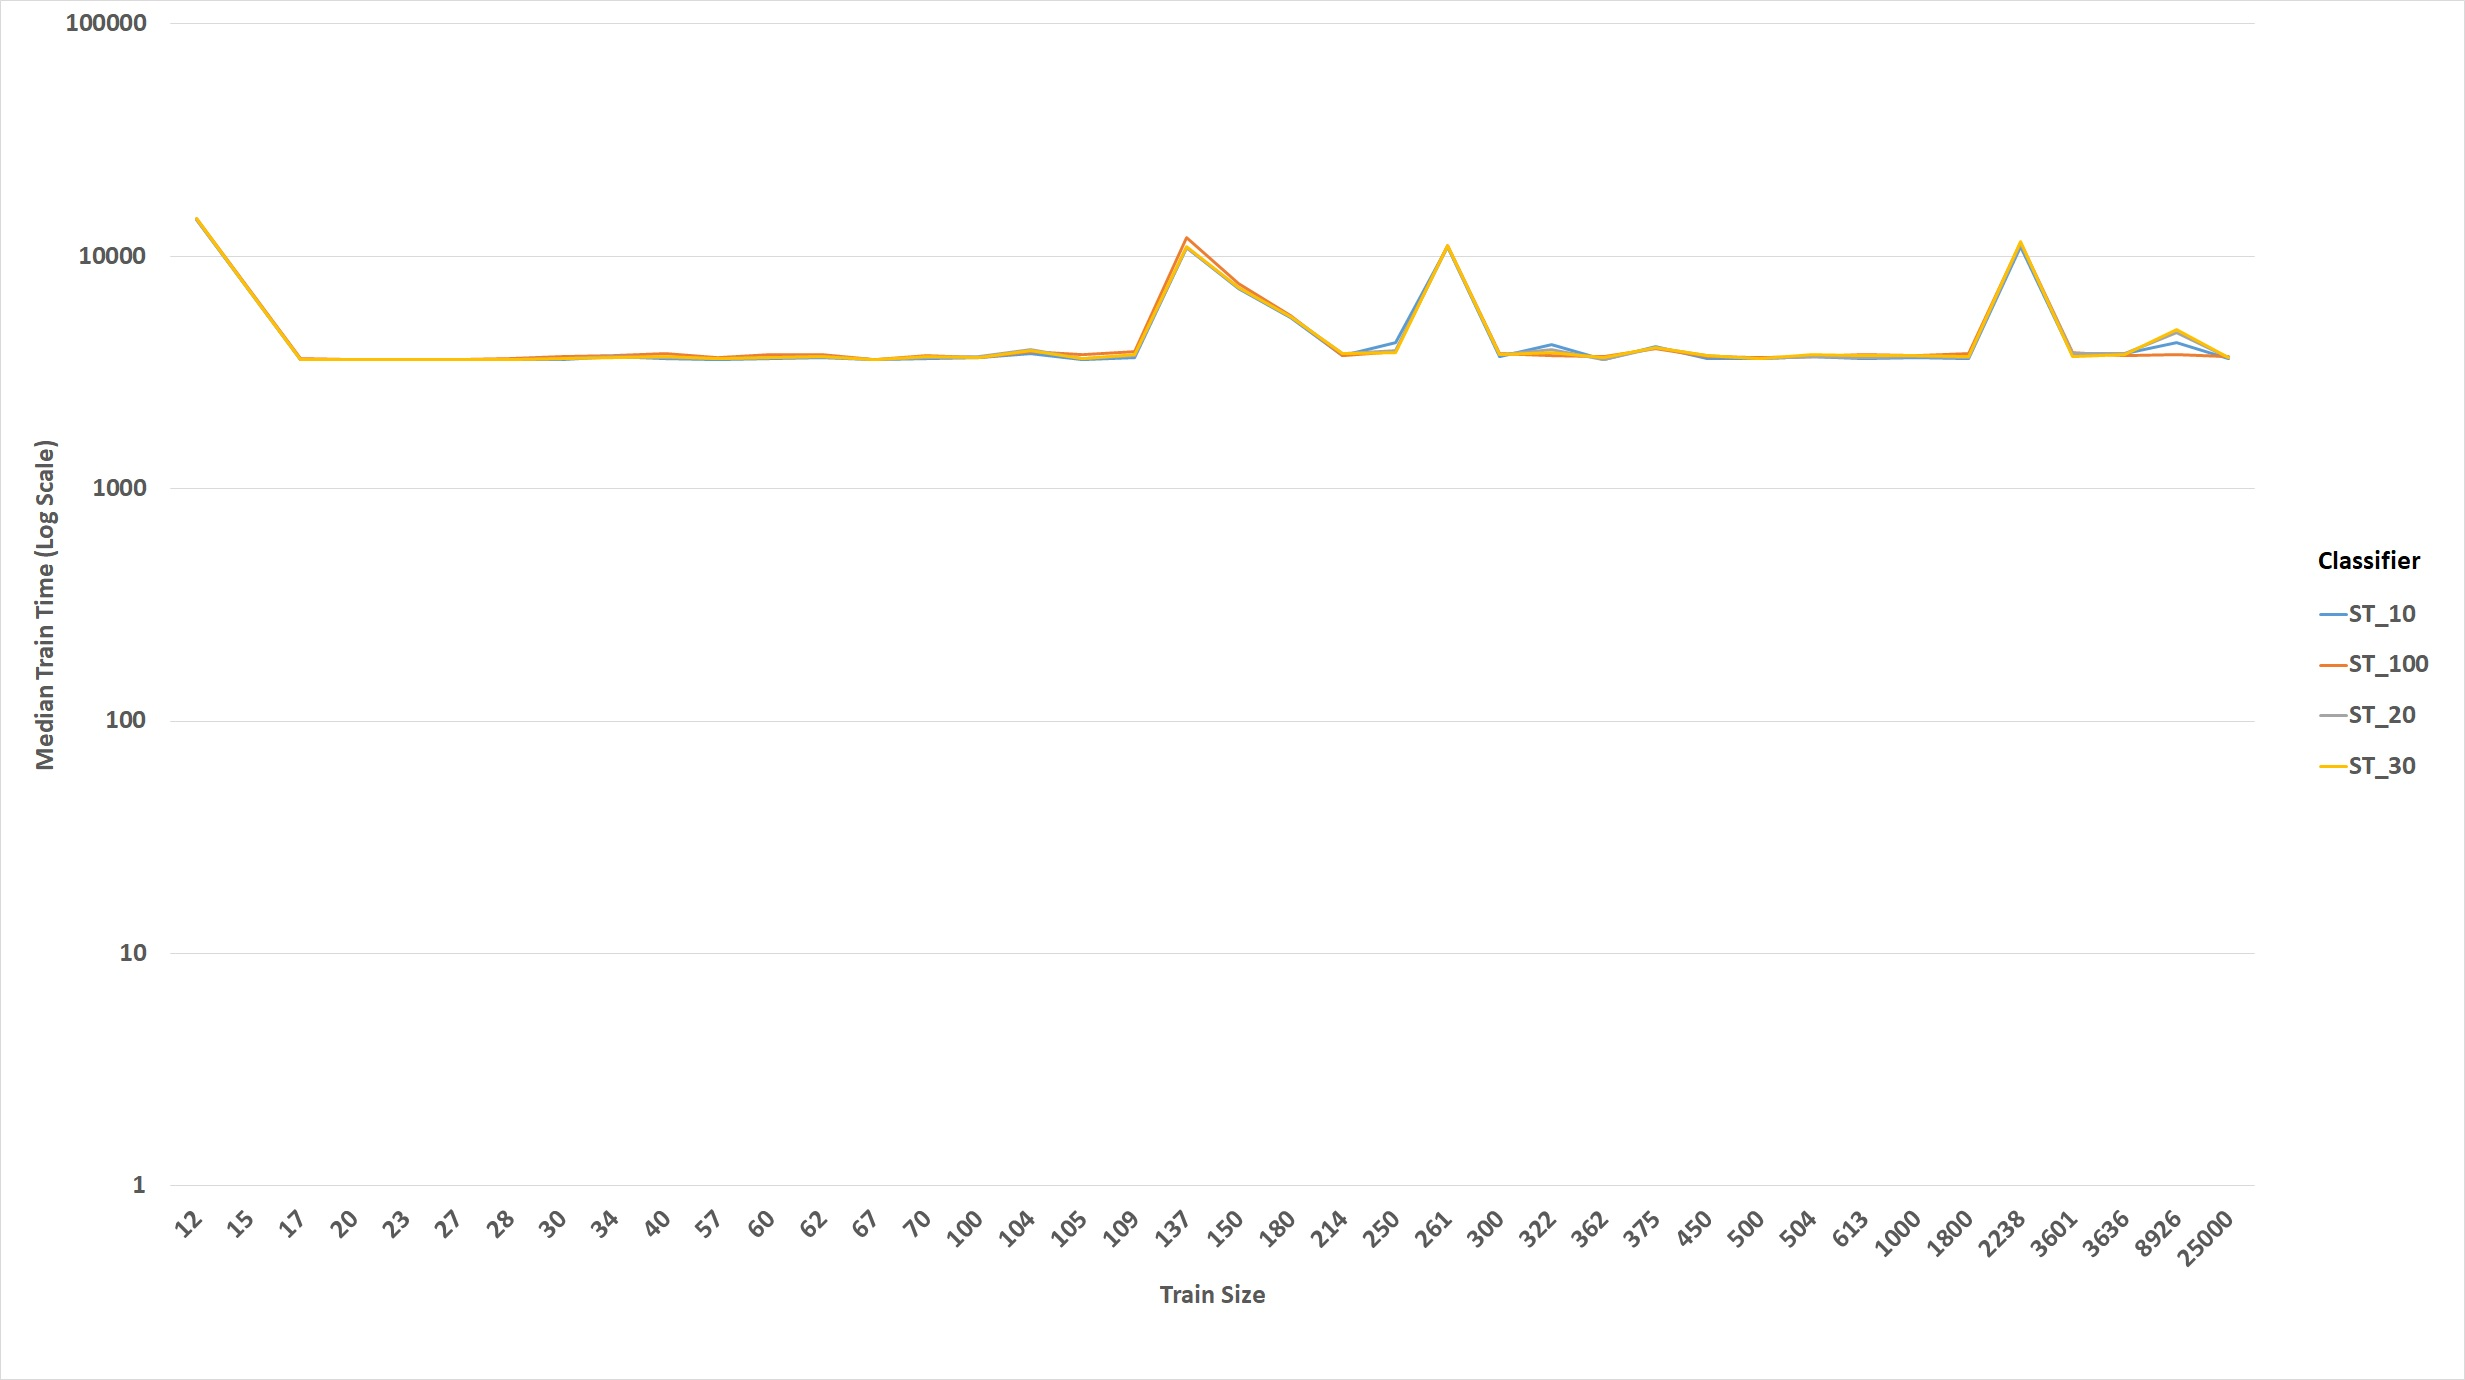
\includegraphics[width=\textwidth]{./Chapters/06 Results/Duration_st_train_size.jpg}
    \caption{Train Time (CPU Time in Log Scale) for ST per train size}
  \end{figure}
  
  \begin{figure} [!htb]
    \centering
    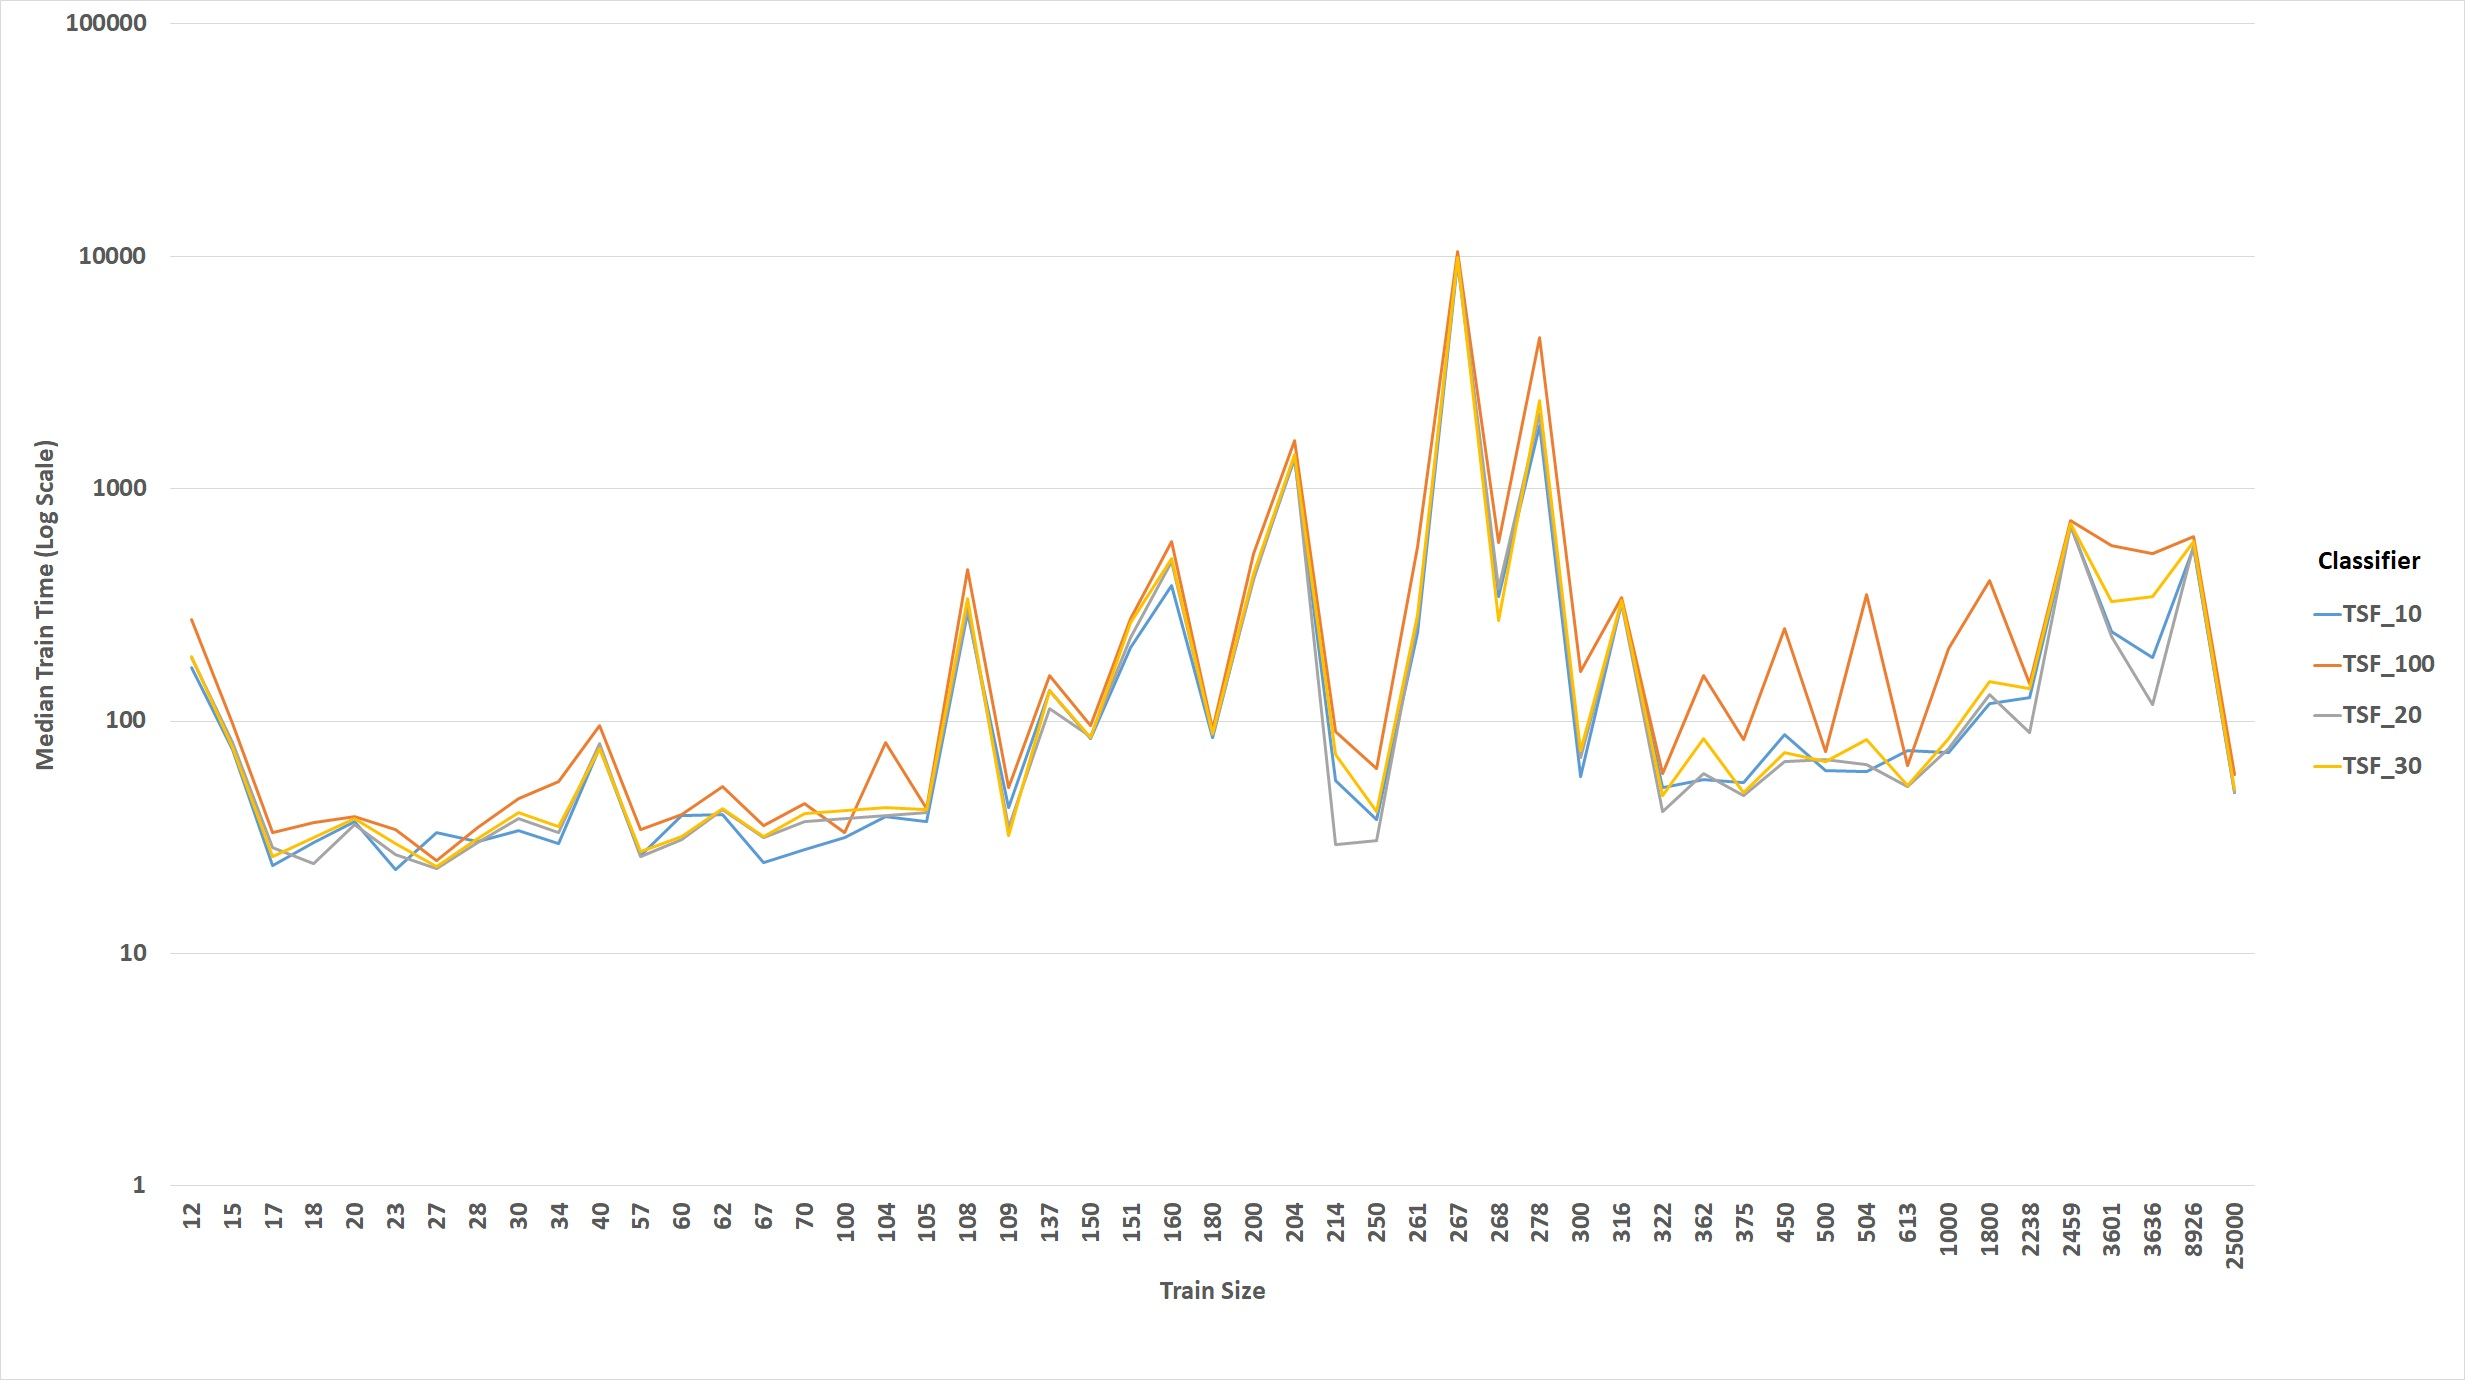
\includegraphics[width=\textwidth]{./Chapters/06 Results/Duration_tsf_train_size.jpg}
    \caption{Train Time (CPU Time in Log Scale) for TSF per train size}
  \end{figure}

  \begin{figure} [!htb]
    \centering
    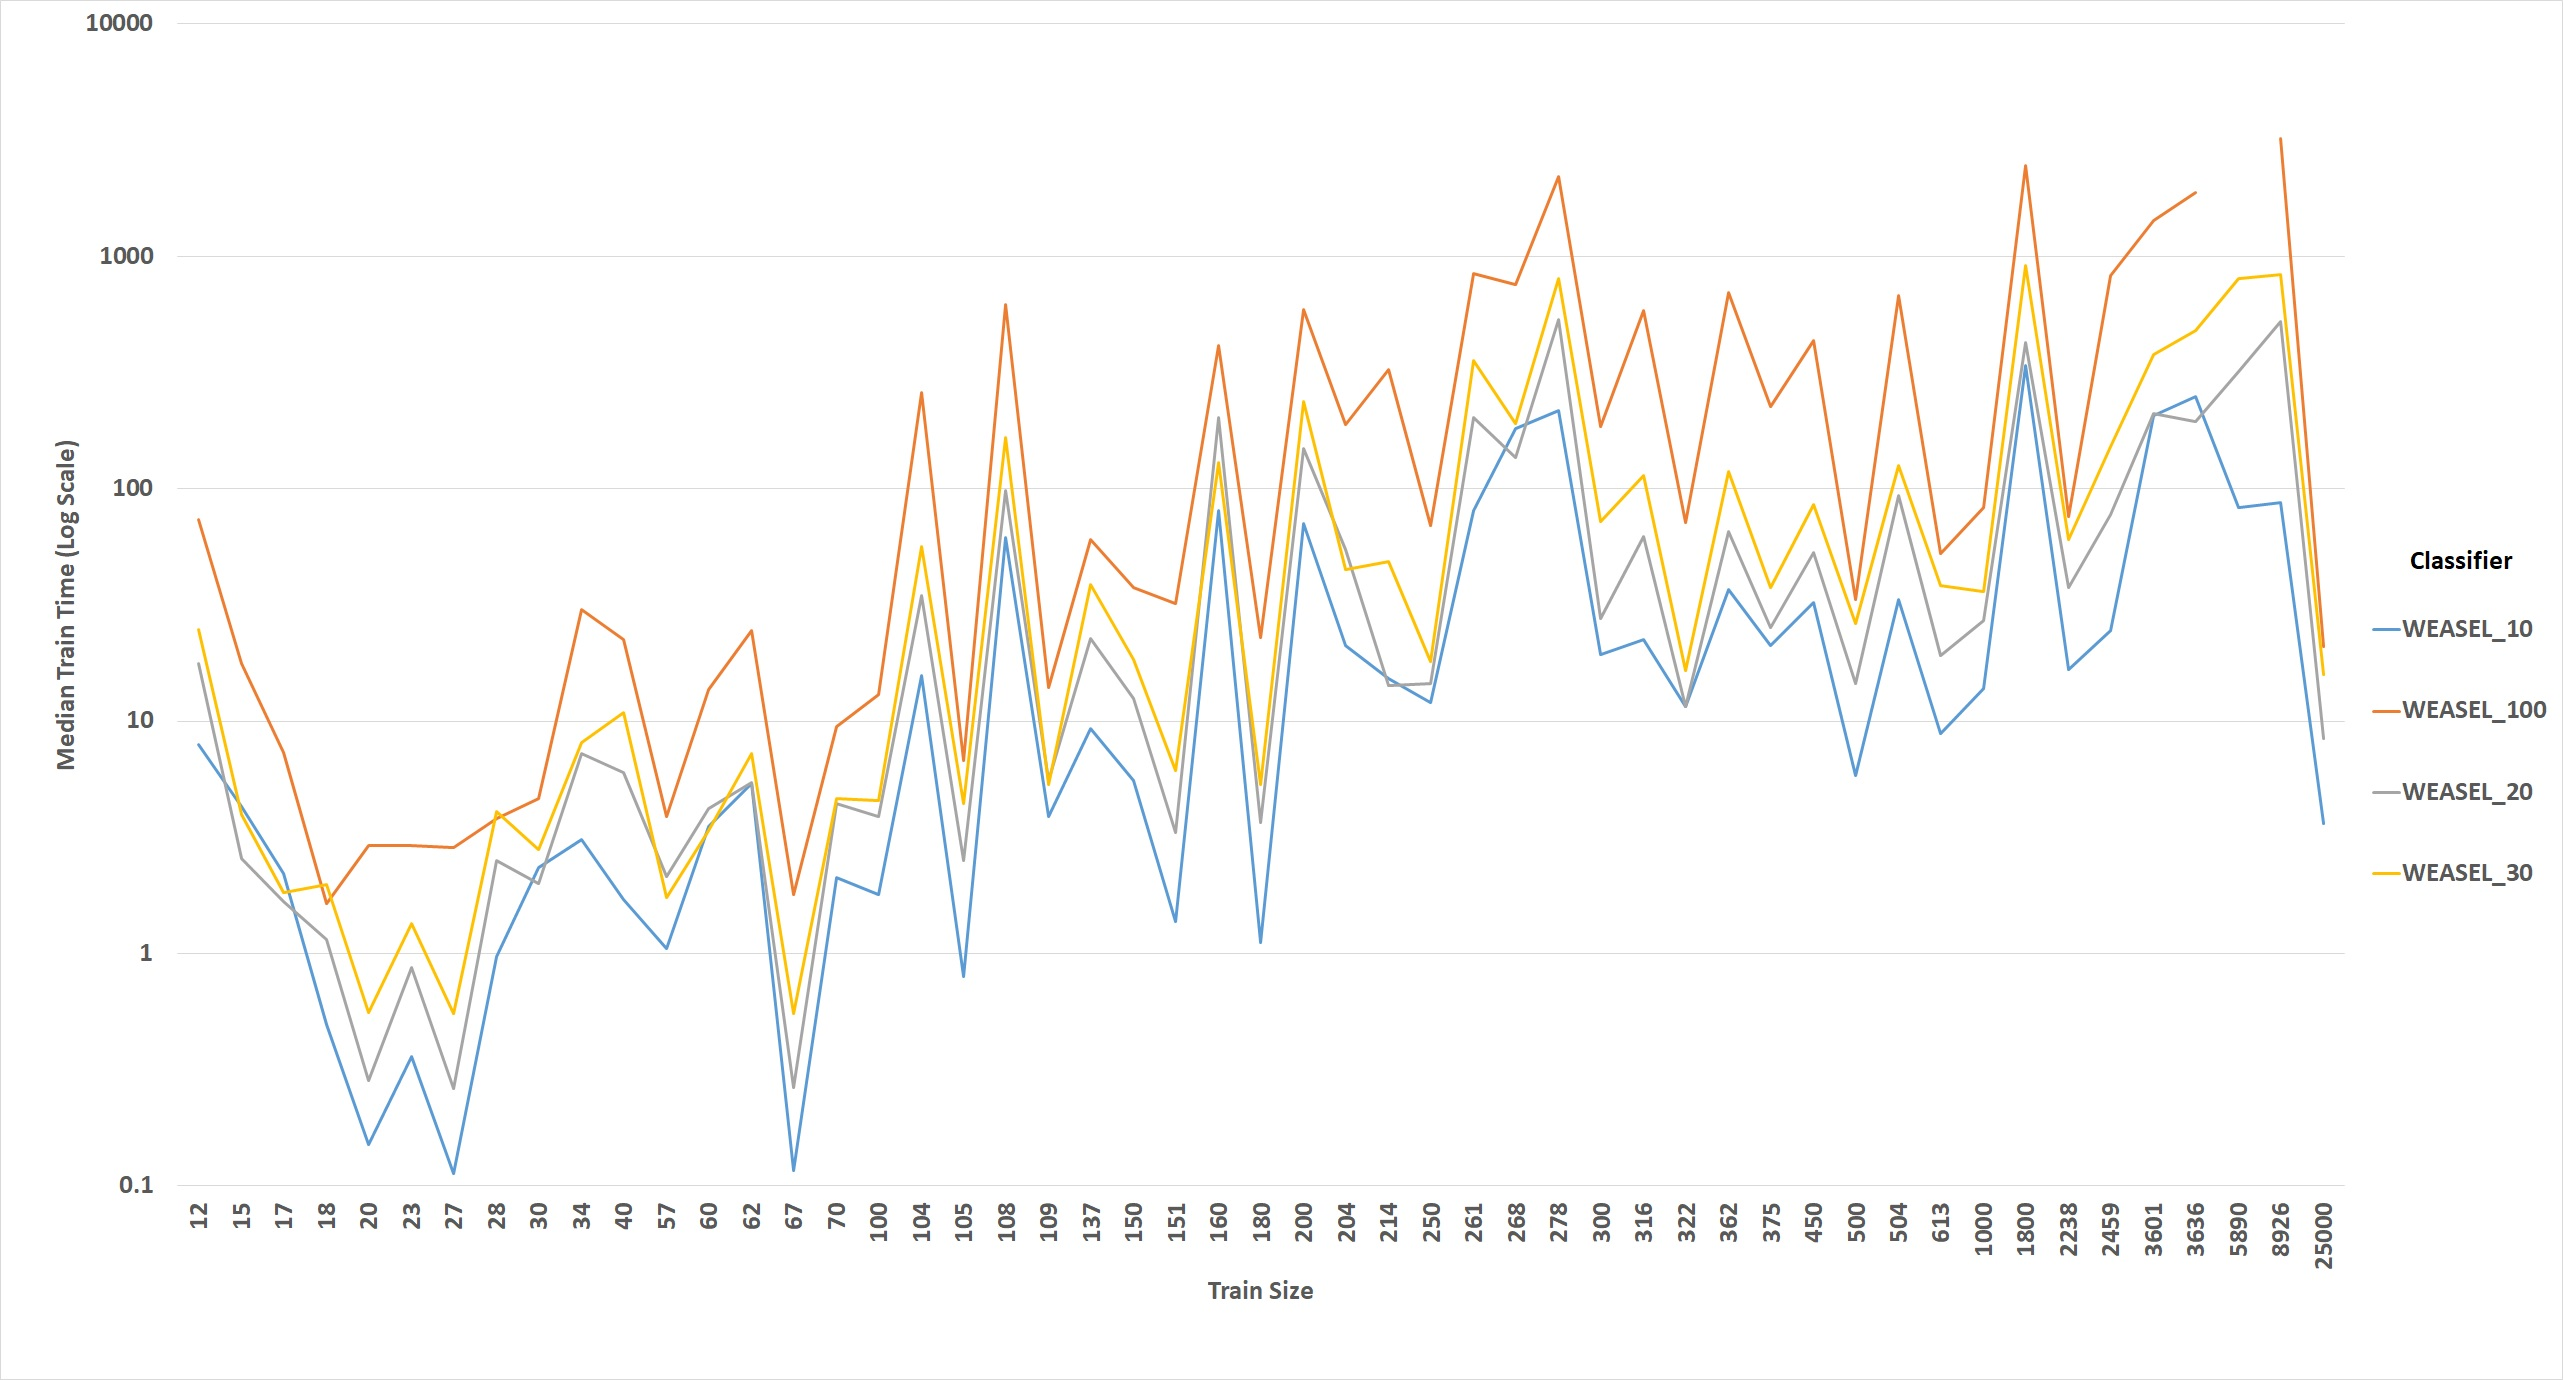
\includegraphics[width=\textwidth]{./Chapters/06 Results/Duration_weasel_train_size.jpg}
    \caption{Train Time (CPU Time in Log Scale) for WEASEL per train size}
  \end{figure}

  %%%%%%%%%%%%%
  %dim
  %%%%%%%%%%%%%
  \begin{figure} [!htb]
    \centering
    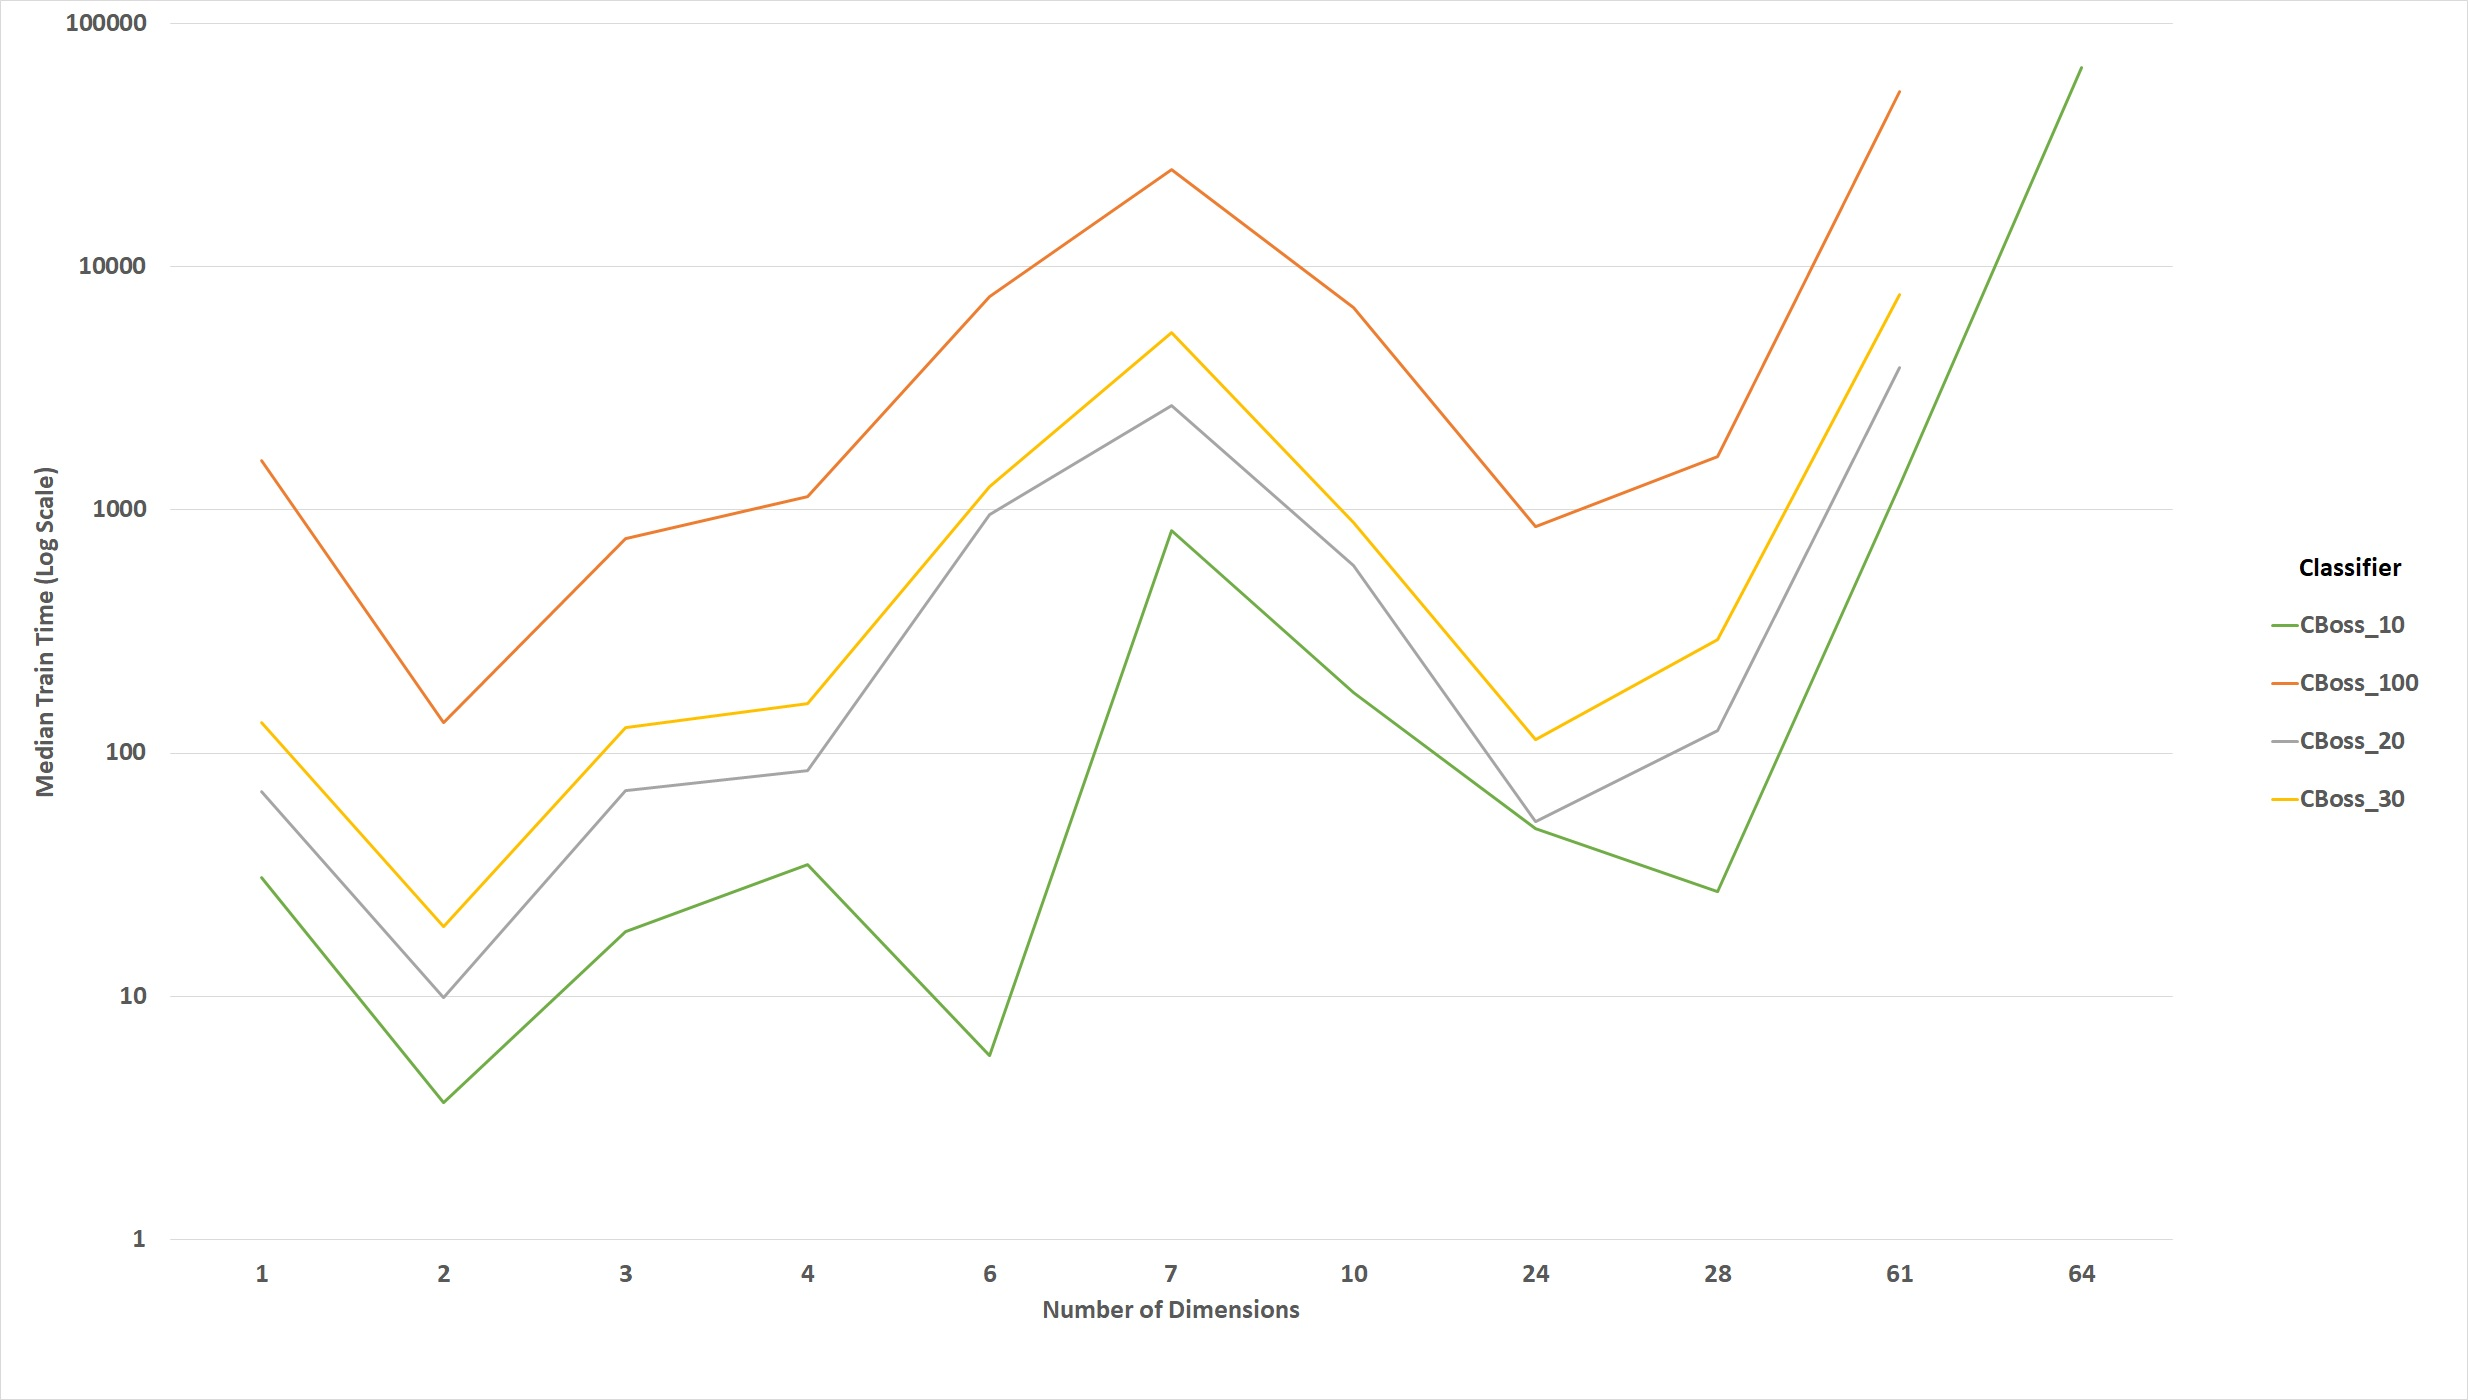
\includegraphics[width=\textwidth]{./Chapters/06 Results/Duration_cboss_dim.jpg}
    \caption{Train Time (CPU Time in Log Scale) for CBOss per number of dimensions}
  \end{figure}
  
  \begin{figure} [!htb]
    \centering
    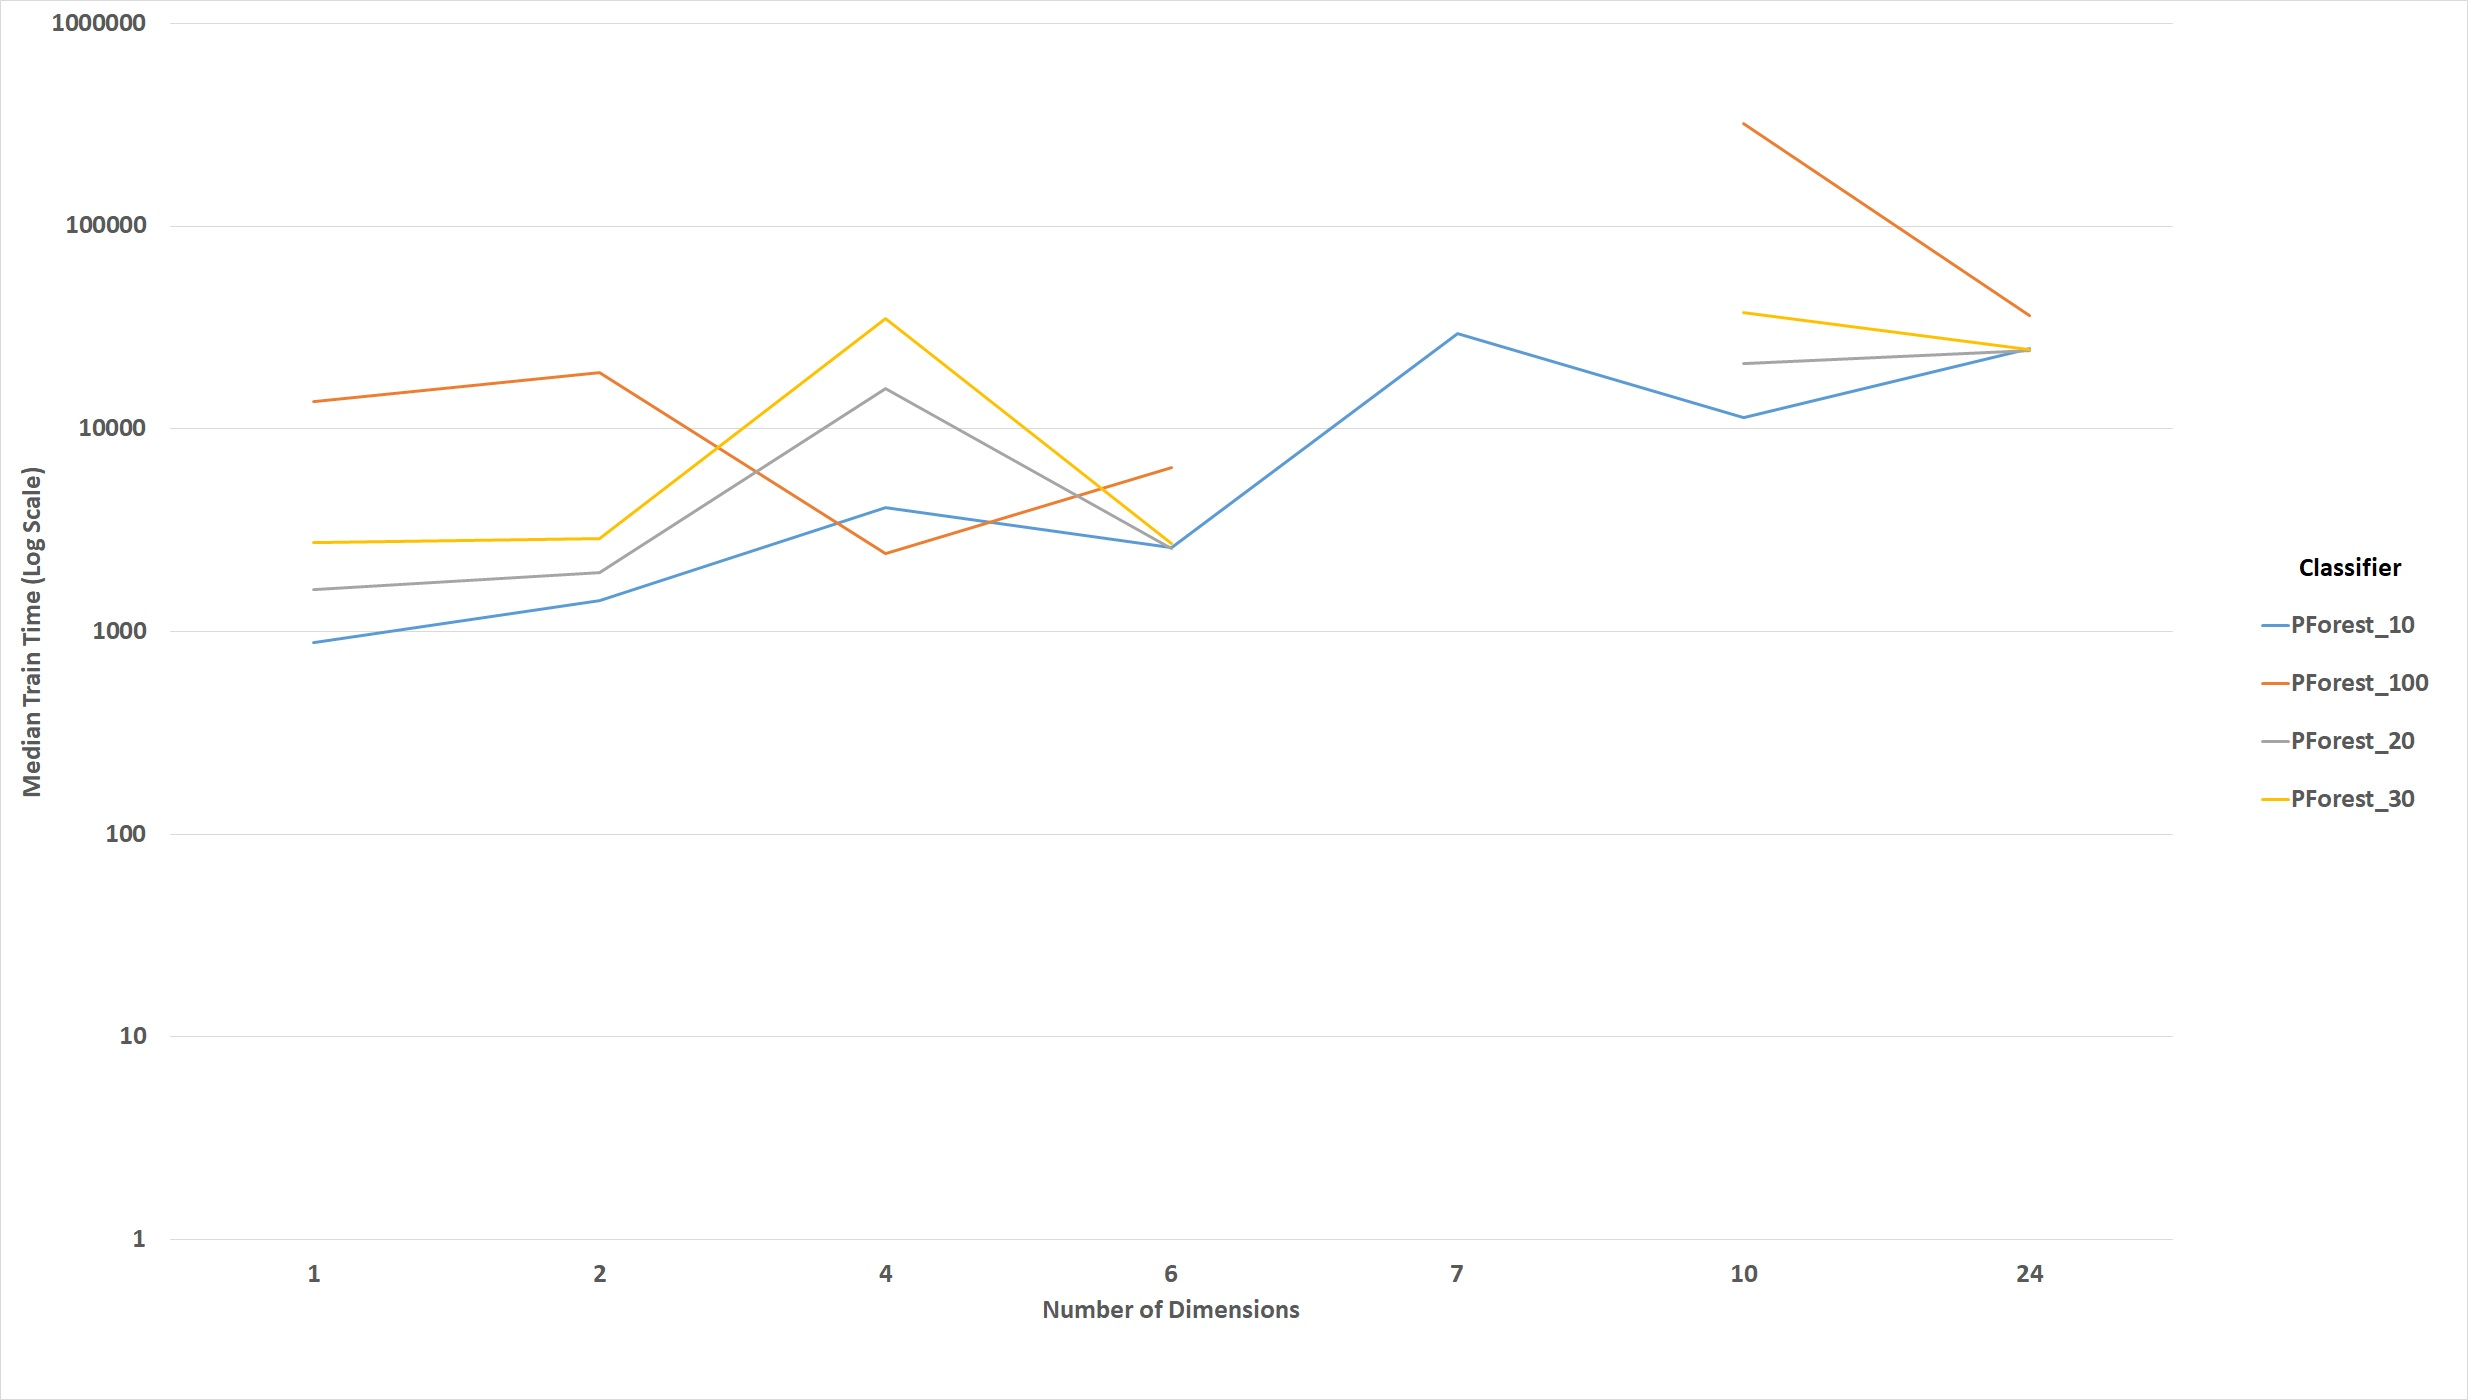
\includegraphics[width=\textwidth]{./Chapters/06 Results/Duration_pforest_dim.jpg}
    \caption{Train Time (CPU Time in Log Scale) for PForest per number of dimensions}
  \end{figure}
  
  \begin{figure} [!htb]
    \centering
    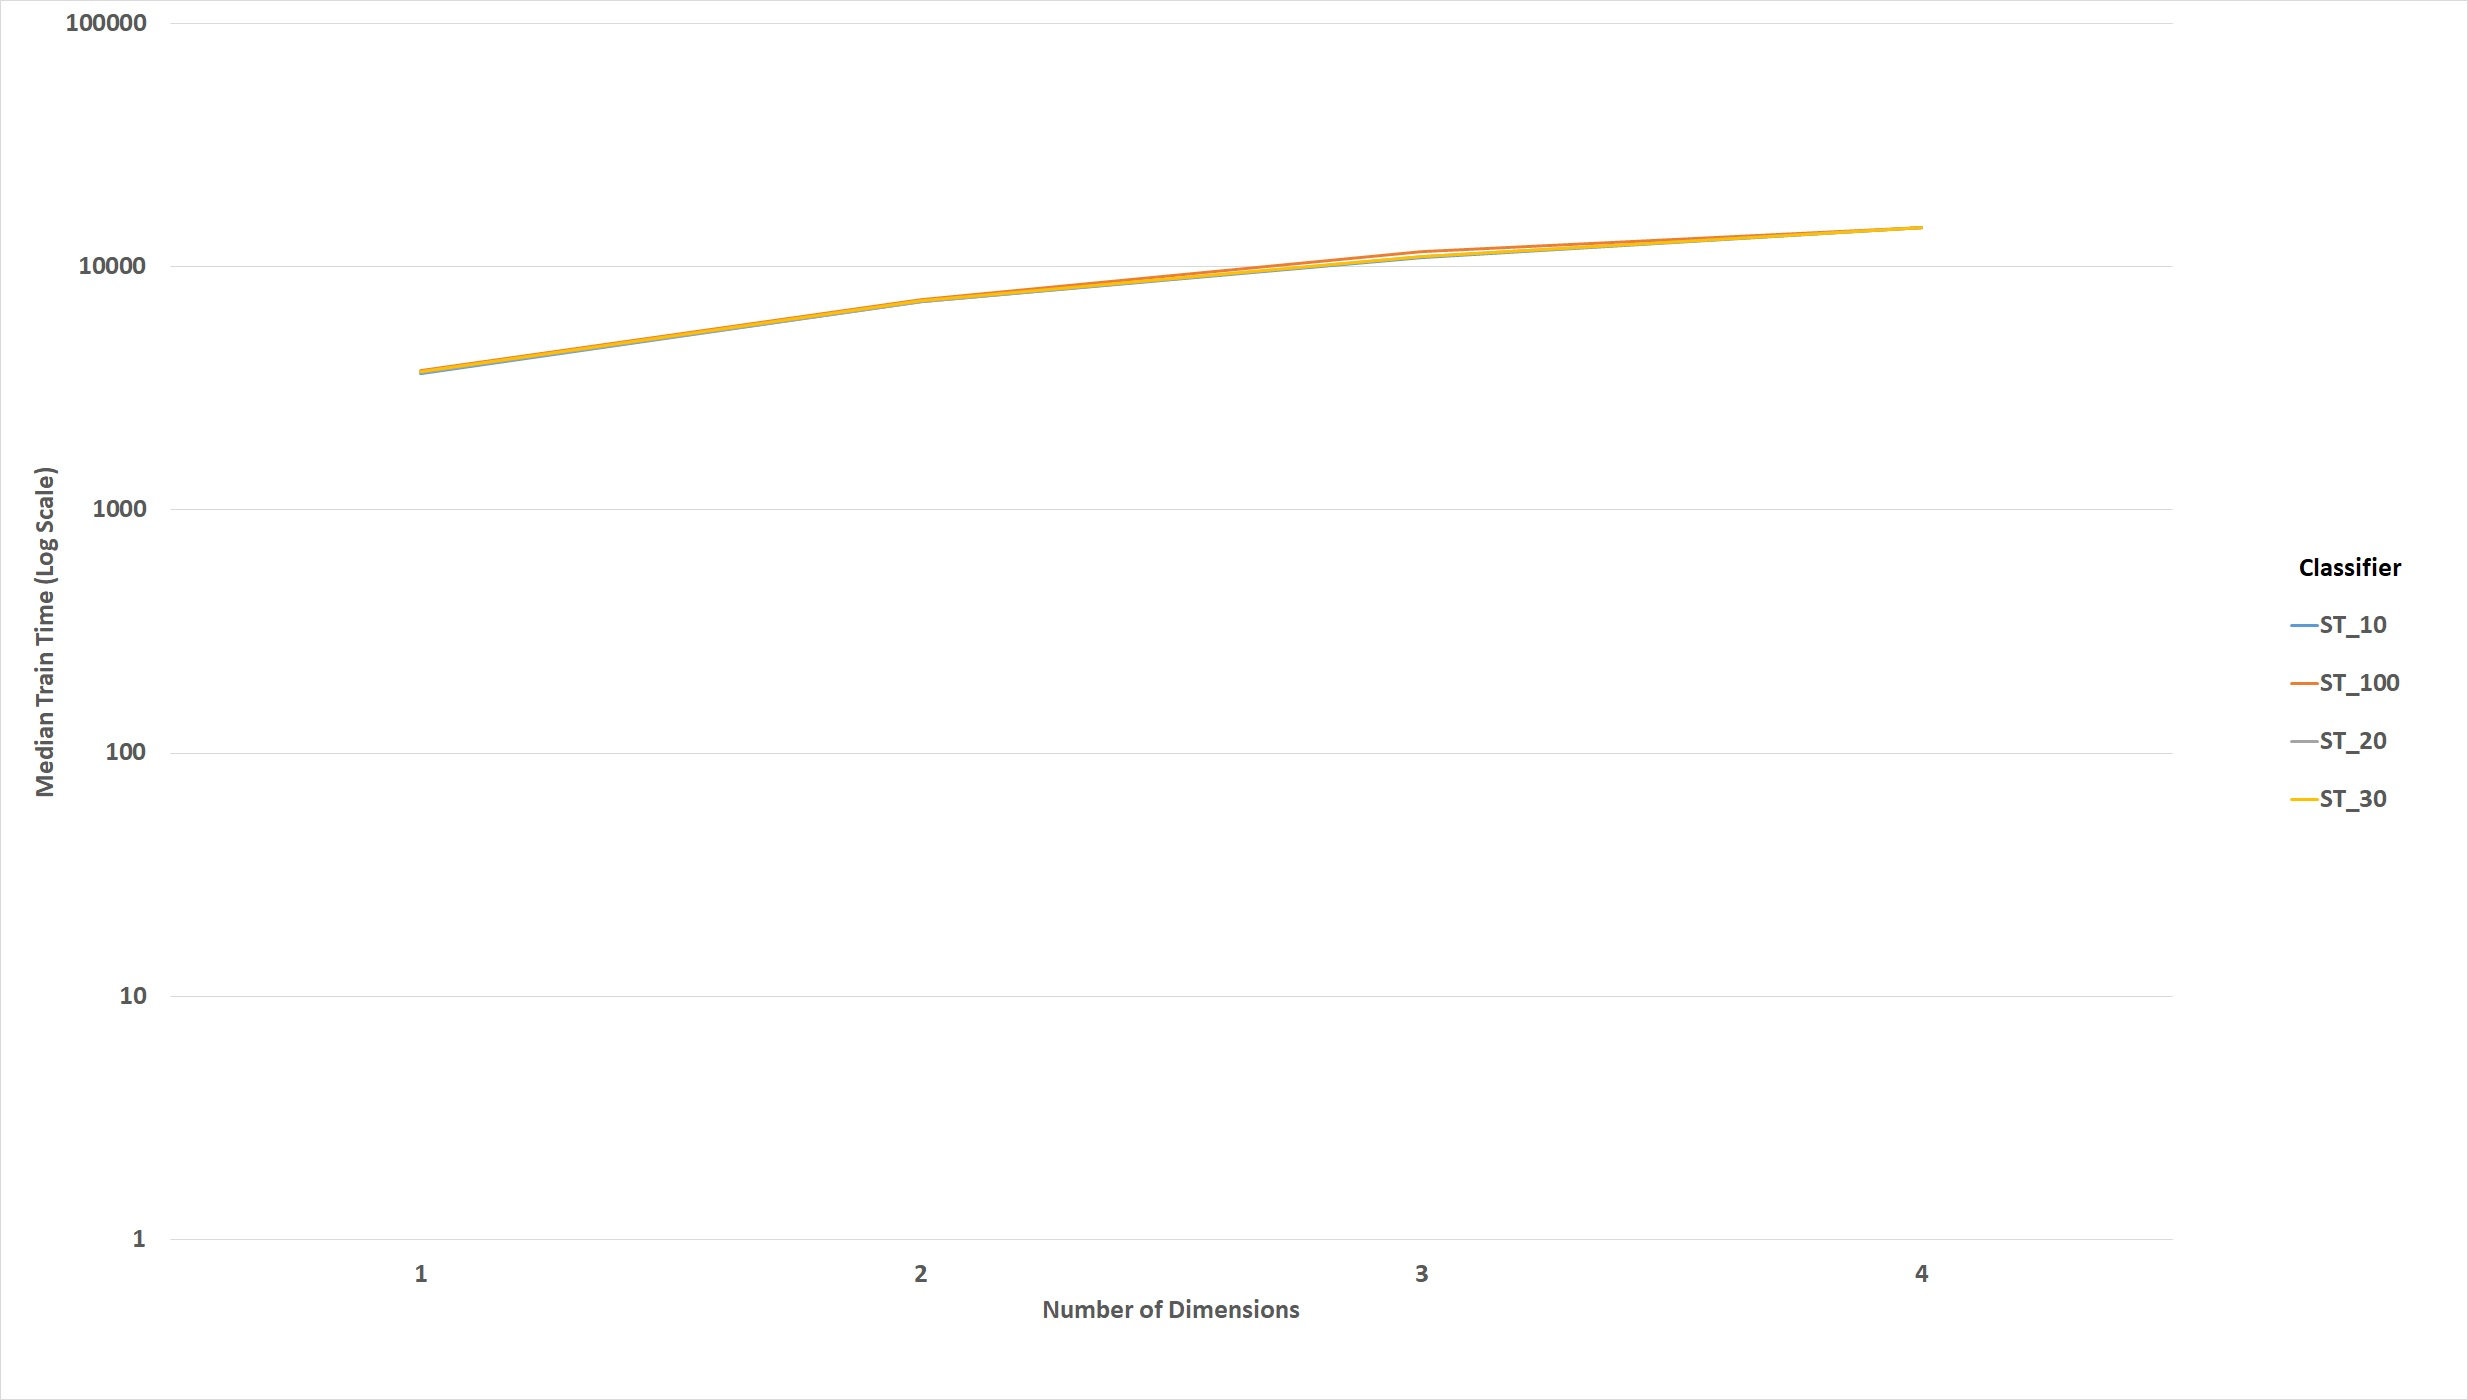
\includegraphics[width=\textwidth]{./Chapters/06 Results/Duration_st_dim.jpg}
    \caption{Train Time (CPU Time in Log Scale) for ST per number of dimensions}
  \end{figure}
  
  \begin{figure} [!htb]
    \centering
    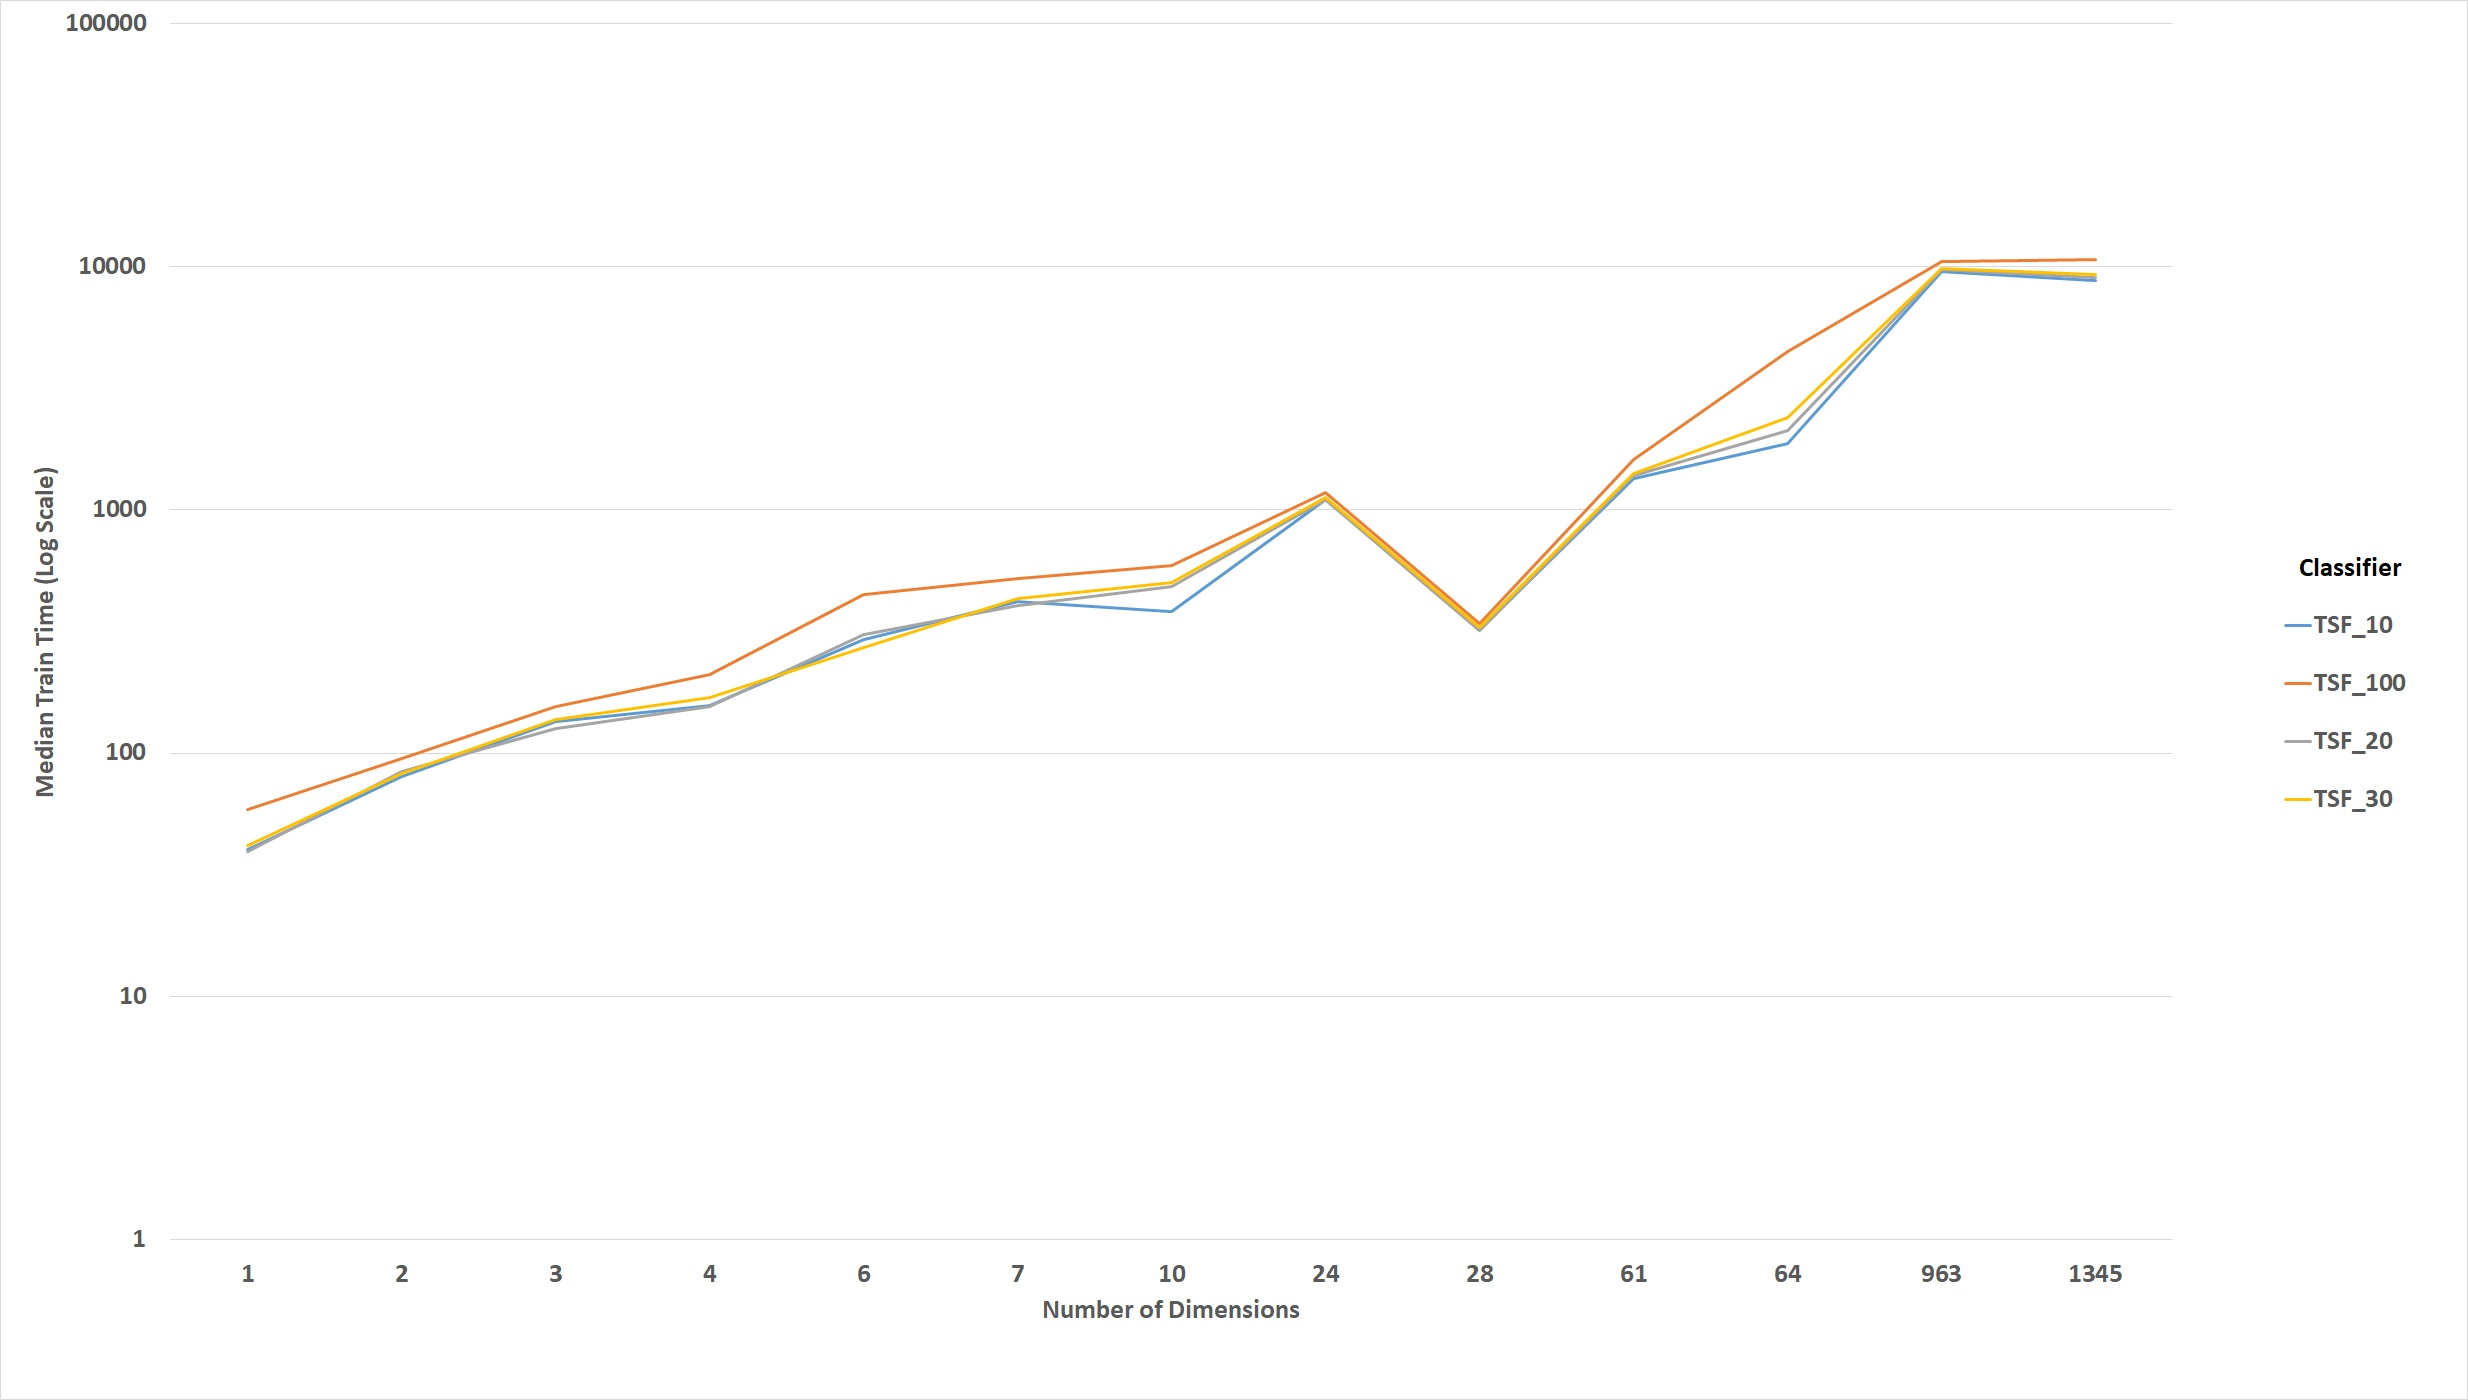
\includegraphics[width=\textwidth]{./Chapters/06 Results/Duration_tsf_dim.jpg}
    \caption{Train Time (CPU Time in Log Scale) for TSF per number of dimensions}
  \end{figure}

  \begin{figure} [!htb]
    \centering
    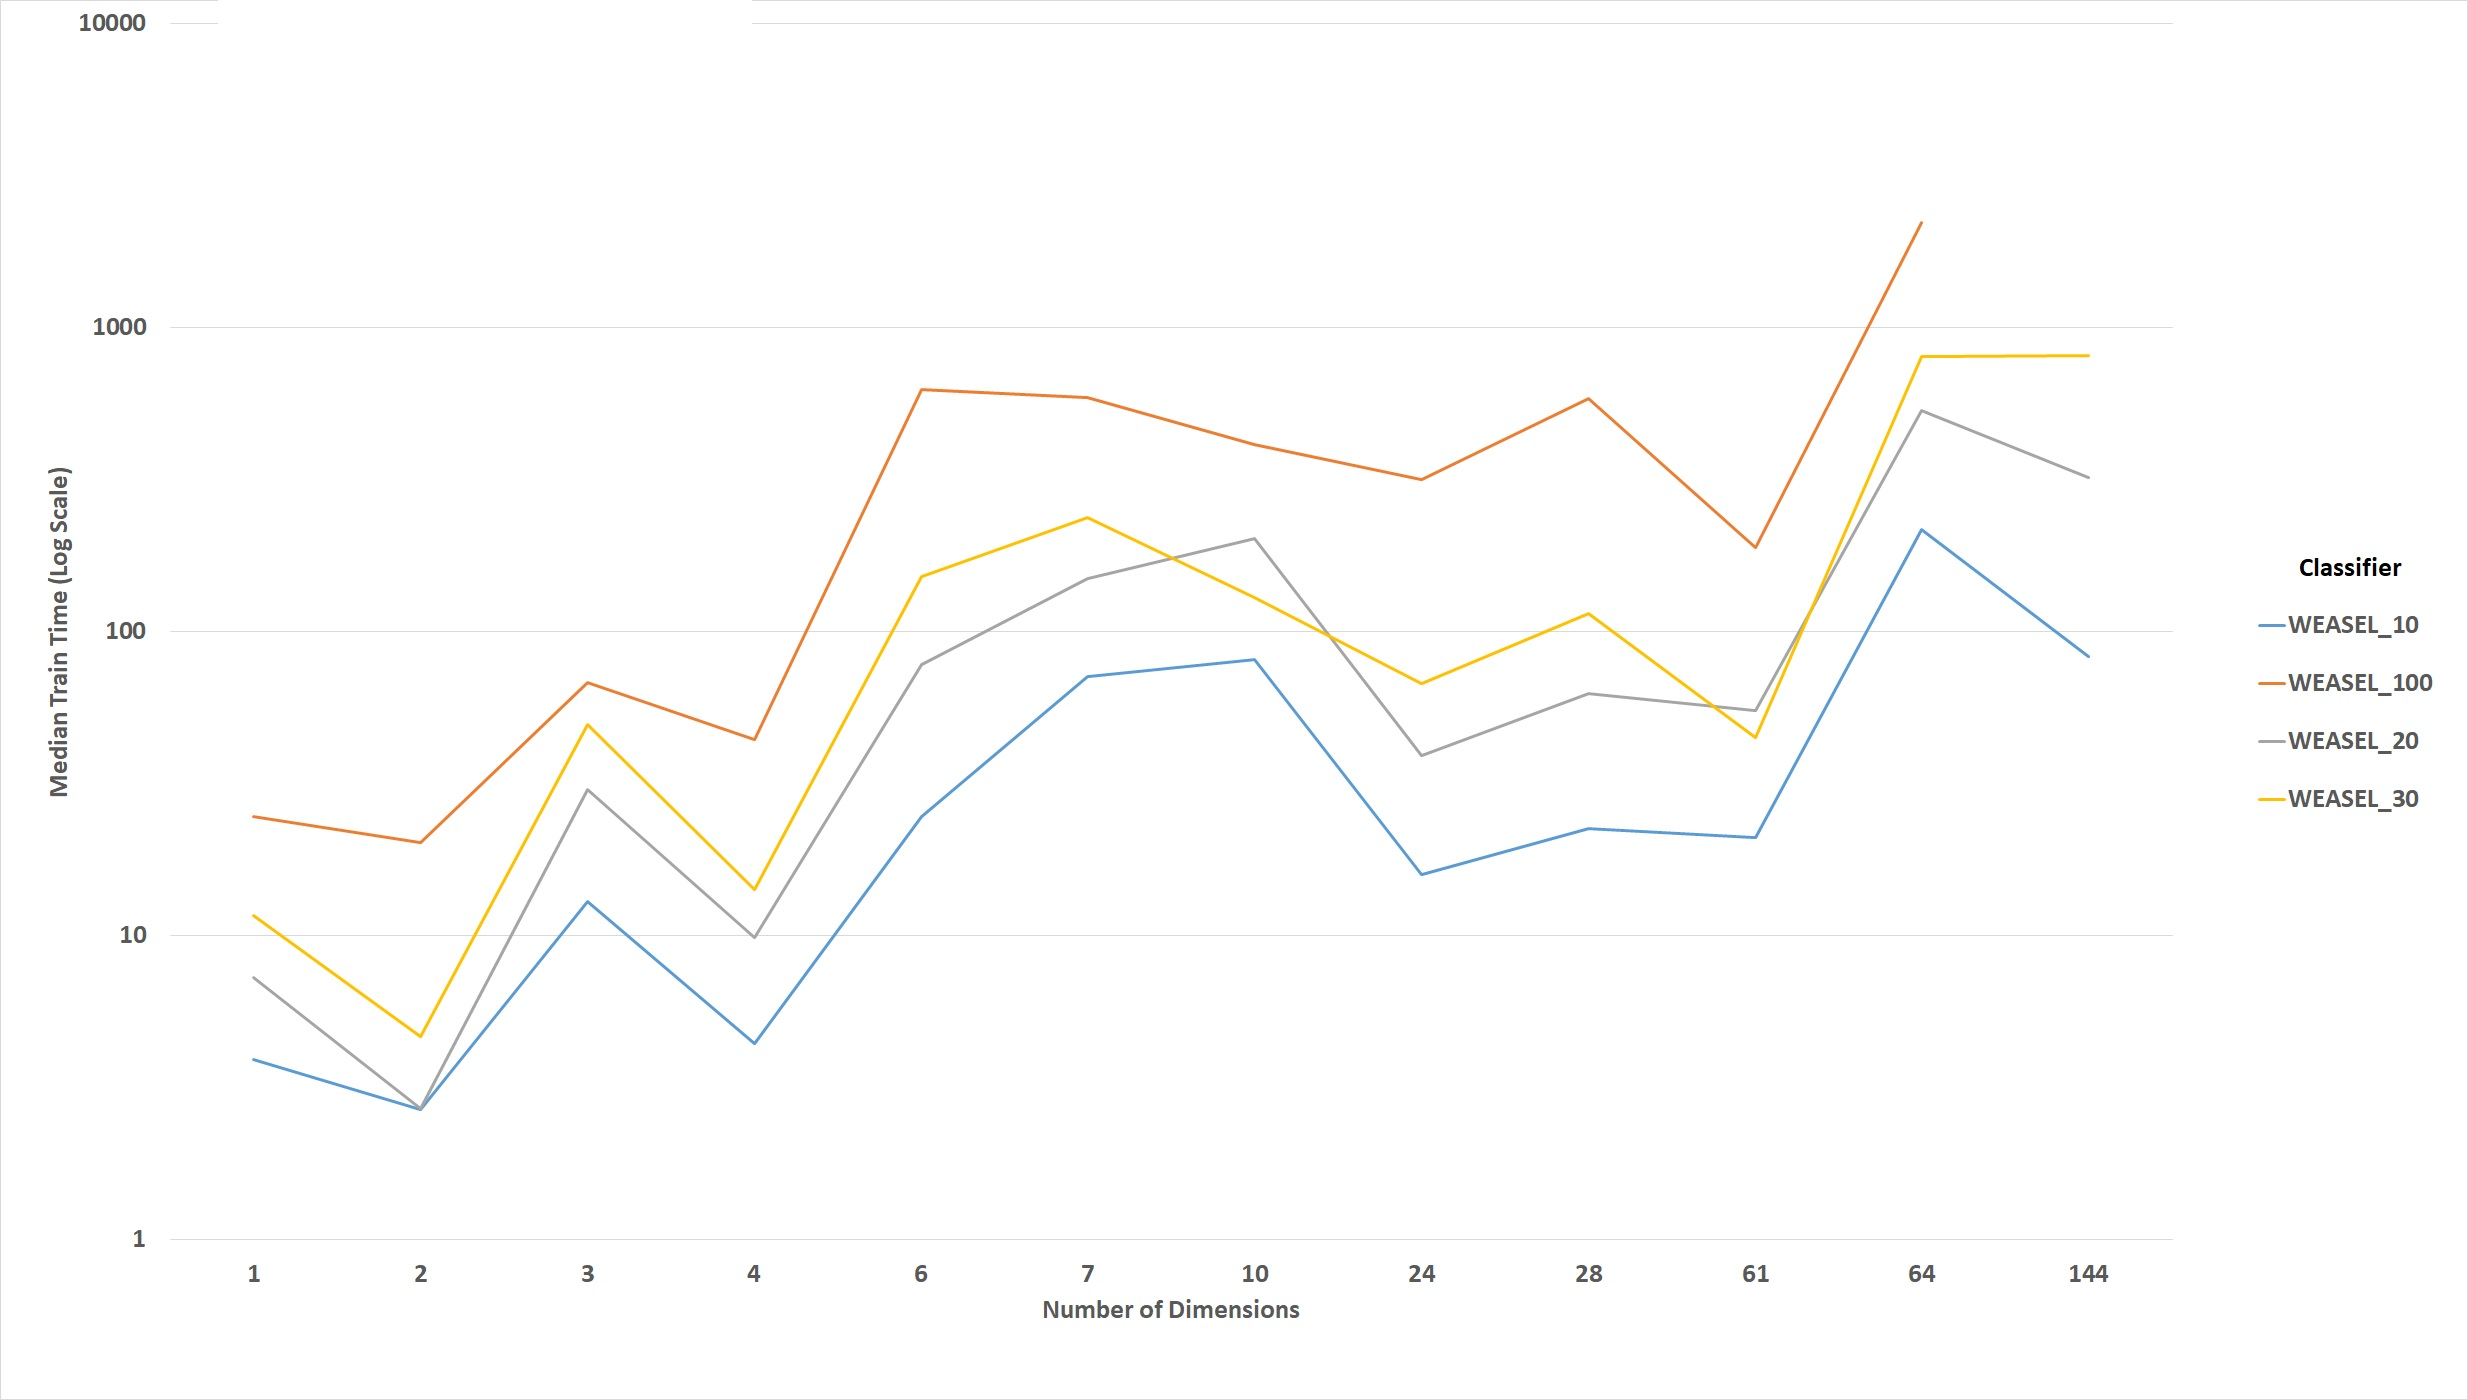
\includegraphics[width=\textwidth]{./Chapters/06 Results/Duration_weasel_dim.jpg}
    \caption{Train Time (CPU Time in Log Scale) for WEASEL per number of dimensions}
  \end{figure}



\chapter{Recommender Results}
  \section{Are the chunk learners able to learn F-scores for the classifiers ?}

  \begin{longtable}{ |c|c|c|c|c| }
    \textbf{\#Seed} & \textbf{Revealed\%} & \textbf{MAE} & \textbf{RMSE} & \textbf{$R^{2}$} \\ [0.5ex]
    \hline
    \endfirsthead % <-- This denotes the end of the header, which will be shown on the first page only
    \hline
    \textbf{\#Seed} & \textbf{Revealed\%} & \textbf{MAE} & \textbf{RMSE} & \textbf{$R^{2}$} \\ [0.5ex]
    \hline
    \endhead
            0 & 10 & 0.059 & 0.087 & 0.046 \\ \hline
            0 & 20 & 0.098 & 0.129 & 0.340 \\ \hline
            0 & 30 & 0.109 & 0.149 & 0.462 \\ \hline
            0 & 100 & 0.125 & 0.169 & 0.664 \\ \hline
            1 & 10 & 0.057 & 0.079 & 0.108 \\ \hline
            1 & 20 & 0.122 & 0.150 & 0.079 \\ \hline
            1 & 30 & 0.134 & 0.165 & 0.254 \\ \hline
            1 & 100 & 0.168 & 0.207 & 0.371 \\ \hline
            2 & 10 & 0.035 & 0.049 & 0.314 \\ \hline
            2 & 20 & 0.086 & 0.111 & 0.385 \\ \hline
            2 & 30 & 0.110 & 0.143 & 0.321 \\ \hline
            2 & 100 & 0.150 & 0.189 & 0.544 \\ \hline
            3 & 10 & 0.070 & 0.102 & 0.155 \\ \hline
            3 & 20 & 0.110 & 0.149 & 0.268 \\ \hline
            3 & 30 & 0.123 & 0.177 & 0.321 \\ \hline
            3 & 100 & 0.176 & 0.217 & 0.511 \\ \hline
            4 & 10 & 0.049 & 0.068 & 0.010 \\ \hline
            4 & 20 & 0.104 & 0.145 & 0.110 \\ \hline
            4 & 30 & 0.137 & 0.186 & 0.065 \\ \hline
            4 & 100 & 0.164 & 0.230 & 0.366 \\ \hline
            5 & 10 & 0.048 & 0.059 & 0.529 \\ \hline
            5 & 20 & 0.093 & 0.113 & 0.443 \\ \hline
            5 & 30 & 0.118 & 0.139 & 0.462 \\ \hline
            5 & 100 & 0.167 & 0.189 & 0.546 \\ \hline
            6 & 10 & 0.049 & 0.063 & 0.396 \\ \hline
            6 & 20 & 0.098 & 0.119 & 0.309 \\ \hline
            6 & 30 & 0.131 & 0.173 & 0.085 \\ \hline
            6 & 100 & 0.136 & 0.169 & 0.556 \\ \hline
            7 & 10 & 0.058 & 0.083 & 0.011 \\ \hline
            7 & 20 & 0.135 & 0.174 & -0.050 \\ \hline
            7 & 30 & 0.165 & 0.209 & 0.044 \\ \hline
            7 & 100 & 0.197 & 0.238 & 0.382 \\ \hline
            8 & 10 & 0.043 & 0.054 & 0.330 \\ \hline
            8 & 20 & 0.099 & 0.116 & 0.339 \\ \hline
            8 & 30 & 0.122 & 0.146 & 0.366 \\ \hline
            8 & 100 & 0.157 & 0.202 & 0.401 \\ \hline
            9 & 10 & 0.045 & 0.056 & 0.516 \\ \hline
            9 & 20 & 0.082 & 0.101 & 0.464 \\ \hline
            9 & 30 & 0.097 & 0.118 & 0.529 \\ \hline
            9 & 100 & 0.138 & 0.180 & 0.515 \\ \hline
            10 & 10 & 0.050 & 0.072 & 0.449 \\ \hline
            10 & 20 & 0.097 & 0.120 & 0.487 \\ \hline
            10 & 30 & 0.112 & 0.139 & 0.515 \\ \hline
            10 & 100 & 0.160 & 0.198 & 0.506 \\ \hline
            11 & 10 & 0.049 & 0.075 & 0.006 \\ \hline
            11 & 20 & 0.089 & 0.125 & 0.059 \\ \hline
            11 & 30 & 0.123 & 0.162 & 0.138 \\ \hline
            11 & 100 & 0.168 & 0.193 & 0.425 \\ \hline
            12 & 10 & 0.048 & 0.068 & 0.221 \\ \hline
            12 & 20 & 0.088 & 0.112 & 0.349 \\ \hline
            12 & 30 & 0.109 & 0.140 & 0.409 \\ \hline
            12 & 100 & 0.137 & 0.168 & 0.641 \\ \hline
            13 & 10 & 0.051 & 0.071 & 0.465 \\ \hline
            13 & 20 & 0.098 & 0.125 & 0.428 \\ \hline
            13 & 30 & 0.142 & 0.174 & 0.283 \\ \hline
            13 & 100 & 0.157 & 0.194 & 0.540 \\ \hline
            14 & 10 & 0.048 & 0.064 & 0.406 \\ \hline
            14 & 20 & 0.093 & 0.120 & 0.314 \\ \hline
            14 & 30 & 0.115 & 0.139 & 0.407 \\ \hline
            14 & 100 & 0.190 & 0.225 & 0.395 \\ \hline
            15 & 10 & 0.045 & 0.055 & 0.190 \\ \hline
            15 & 20 & 0.111 & 0.130 & 0.283 \\ \hline
            15 & 30 & 0.121 & 0.153 & 0.408 \\ \hline
            15 & 100 & 0.225 & 0.279 & 0.180 \\ \hline
            16 & 10 & 0.045 & 0.071 & 0.338 \\ \hline
            16 & 20 & 0.091 & 0.129 & 0.255 \\ \hline
            16 & 30 & 0.114 & 0.162 & 0.289 \\ \hline
            16 & 100 & 0.148 & 0.196 & 0.561 \\ \hline
            17 & 10 & 0.050 & 0.075 & 0.127 \\ \hline
            17 & 20 & 0.096 & 0.136 & 0.263 \\ \hline
            17 & 30 & 0.135 & 0.183 & 0.149 \\ \hline
            17 & 100 & 0.135 & 0.168 & 0.686 \\ \hline
            18 & 10 & 0.042 & 0.059 & -0.215 \\ \hline
            18 & 20 & 0.092 & 0.117 & -0.122 \\ \hline
            18 & 30 & 0.122 & 0.167 & -0.345 \\ \hline
            18 & 100 & 0.166 & 0.214 & 0.230 \\ \hline
            19 & 10 & 0.040 & 0.054 & 0.588 \\ \hline
            19 & 20 & 0.076 & 0.097 & 0.577 \\ \hline
            19 & 30 & 0.096 & 0.122 & 0.594 \\ \hline
            19 & 100 & 0.136 & 0.181 & 0.624 \\ \hline
            20 & 10 & 0.058 & 0.088 & 0.265 \\ \hline
            20 & 20 & 0.111 & 0.148 & 0.246 \\ \hline
            20 & 30 & 0.139 & 0.180 & 0.291 \\ \hline
            20 & 100 & 0.175 & 0.213 & 0.524 \\ \hline
            21 & 10 & 0.045 & 0.066 & 0.302 \\ \hline
            21 & 20 & 0.088 & 0.110 & 0.509 \\ \hline
            21 & 30 & 0.121 & 0.146 & 0.460 \\ \hline
            21 & 100 & 0.172 & 0.249 & 0.360 \\ \hline
            22 & 10 & 0.038 & 0.045 & 0.638 \\ \hline
            22 & 20 & 0.084 & 0.103 & 0.352 \\ \hline
            22 & 30 & 0.098 & 0.124 & 0.350 \\ \hline
            22 & 100 & 0.165 & 0.208 & 0.221 \\ \hline
            23 & 10 & 0.053 & 0.062 & 0.480 \\ \hline
            23 & 20 & 0.093 & 0.117 & 0.488 \\ \hline
            23 & 30 & 0.119 & 0.151 & 0.465 \\ \hline
            23 & 100 & 0.138 & 0.172 & 0.678 \\ \hline
            24 & 10 & 0.037 & 0.067 & 0.040 \\ \hline
            24 & 20 & 0.081 & 0.112 & 0.349 \\ \hline
            24 & 30 & 0.102 & 0.143 & 0.366 \\ \hline
            24 & 100 & 0.148 & 0.192 & 0.549 \\ \hline
            25 & 10 & 0.046 & 0.060 & 0.275 \\ \hline
            25 & 20 & 0.100 & 0.129 & 0.314 \\ \hline
            25 & 30 & 0.141 & 0.171 & 0.175 \\ \hline
            25 & 100 & 0.159 & 0.195 & 0.504 \\ \hline
            26 & 10 & 0.049 & 0.072 & 0.395 \\ \hline
            26 & 20 & 0.092 & 0.118 & 0.527 \\ \hline
            26 & 30 & 0.119 & 0.146 & 0.502 \\ \hline
            26 & 100 & 0.180 & 0.211 & 0.535 \\ \hline
            27 & 10 & 0.046 & 0.064 & 0.026 \\ \hline
            27 & 20 & 0.089 & 0.117 & 0.165 \\ \hline
            27 & 30 & 0.113 & 0.147 & 0.243 \\ \hline
            27 & 100 & 0.127 & 0.155 & 0.660 \\ \hline
            28 & 10 & 0.040 & 0.064 & 0.363 \\ \hline
            28 & 20 & 0.086 & 0.120 & 0.436 \\ \hline
            28 & 30 & 0.105 & 0.140 & 0.483 \\ \hline
            28 & 100 & 0.134 & 0.169 & 0.647 \\ \hline
            29 & 10 & 0.040 & 0.047 & 0.187 \\ \hline
            29 & 20 & 0.091 & 0.110 & 0.278 \\ \hline
            29 & 30 & 0.108 & 0.142 & 0.377 \\ \hline
            29 & 100 & 0.144 & 0.188 & 0.605 \\ \hline
            30 & 10 & 0.047 & 0.062 & 0.489 \\ \hline
            30 & 20 & 0.095 & 0.116 & 0.488 \\ \hline
            30 & 30 & 0.128 & 0.153 & 0.408 \\ \hline
            30 & 100 & 0.147 & 0.190 & 0.596 \\ \hline
            31 & 10 & 0.050 & 0.062 & 0.176 \\ \hline
            31 & 20 & 0.095 & 0.118 & 0.327 \\ \hline
            31 & 30 & 0.127 & 0.154 & 0.369 \\ \hline
            31 & 100 & 0.189 & 0.227 & 0.462 \\ \hline
            32 & 10 & 0.049 & 0.063 & 0.434 \\ \hline
            32 & 20 & 0.097 & 0.120 & 0.410 \\ \hline
            32 & 30 & 0.130 & 0.158 & 0.360 \\ \hline
            32 & 100 & 0.159 & 0.204 & 0.480 \\ \hline
            33 & 10 & 0.049 & 0.063 & -0.369 \\ \hline
            33 & 20 & 0.094 & 0.114 & -0.014 \\ \hline
            33 & 30 & 0.129 & 0.155 & -0.004 \\ \hline
            33 & 100 & 0.177 & 0.209 & 0.312 \\ \hline
            34 & 10 & 0.066 & 0.084 & 0.012 \\ \hline
            34 & 20 & 0.104 & 0.143 & 0.146 \\ \hline
            34 & 30 & 0.125 & 0.157 & 0.315 \\ \hline
            34 & 100 & 0.172 & 0.210 & 0.540 \\ \hline
            35 & 10 & 0.047 & 0.074 & 0.073 \\ \hline
            35 & 20 & 0.098 & 0.137 & 0.111 \\ \hline
            35 & 30 & 0.116 & 0.168 & 0.139 \\ \hline
            35 & 100 & 0.135 & 0.164 & 0.667 \\ \hline
            36 & 10 & 0.047 & 0.059 & 0.439 \\ \hline
            36 & 20 & 0.110 & 0.146 & -0.019 \\ \hline
            36 & 30 & 0.115 & 0.142 & 0.366 \\ \hline
            36 & 100 & 0.151 & 0.190 & 0.461 \\ \hline
            37 & 10 & 0.039 & 0.055 & 0.028 \\ \hline
            37 & 20 & 0.088 & 0.115 & 0.054 \\ \hline
            37 & 30 & 0.132 & 0.175 & -0.173 \\ \hline
            37 & 100 & 0.121 & 0.155 & 0.663 \\ \hline
            38 & 10 & 0.048 & 0.061 & 0.134 \\ \hline
            38 & 20 & 0.077 & 0.096 & 0.392 \\ \hline
            38 & 30 & 0.100 & 0.125 & 0.449 \\ \hline
            38 & 100 & 0.145 & 0.179 & 0.625 \\ \hline
            39 & 10 & 0.056 & 0.080 & 0.336 \\ \hline
            39 & 20 & 0.106 & 0.136 & 0.380 \\ \hline
            39 & 30 & 0.133 & 0.161 & 0.436 \\ \hline
            39 & 100 & 0.165 & 0.214 & 0.532 \\ \hline
            40 & 10 & 0.045 & 0.060 & 0.464 \\ \hline
            40 & 20 & 0.081 & 0.099 & 0.523 \\ \hline
            40 & 30 & 0.103 & 0.128 & 0.495 \\ \hline
            40 & 100 & 0.111 & 0.137 & 0.721 \\ \hline
            41 & 10 & 0.041 & 0.056 & 0.084 \\ \hline
            41 & 20 & 0.092 & 0.126 & 0.164 \\ \hline
            41 & 30 & 0.132 & 0.162 & 0.250 \\ \hline
            41 & 100 & 0.165 & 0.198 & 0.535 \\ \hline
            42 & 10 & 0.054 & 0.075 & 0.283 \\ \hline
            42 & 20 & 0.102 & 0.122 & 0.343 \\ \hline
            42 & 30 & 0.124 & 0.148 & 0.329 \\ \hline
            42 & 100 & 0.139 & 0.175 & 0.500 \\ \hline
            43 & 10 & 0.039 & 0.048 & 0.295 \\ \hline
            43 & 20 & 0.081 & 0.111 & 0.252 \\ \hline
            43 & 30 & 0.095 & 0.135 & 0.357 \\ \hline
            43 & 100 & 0.151 & 0.177 & 0.614 \\ \hline
            44 & 10 & 0.044 & 0.067 & -0.021 \\ \hline
            44 & 20 & 0.103 & 0.144 & -0.186 \\ \hline
            44 & 30 & 0.126 & 0.163 & 0.086 \\ \hline
            44 & 100 & 0.125 & 0.161 & 0.705 \\ \hline
            45 & 10 & 0.049 & 0.076 & 0.150 \\ \hline
            45 & 20 & 0.108 & 0.138 & 0.295 \\ \hline
            45 & 30 & 0.124 & 0.169 & 0.360 \\ \hline
            45 & 100 & 0.166 & 0.206 & 0.573 \\ \hline
            46 & 10 & 0.074 & 0.099 & -0.935 \\ \hline
            46 & 20 & 0.125 & 0.165 & -0.558 \\ \hline
            46 & 30 & 0.142 & 0.181 & 0.025 \\ \hline
            46 & 100 & 0.184 & 0.246 & 0.308 \\ \hline
            47 & 10 & 0.046 & 0.063 & 0.212 \\ \hline
            47 & 20 & 0.083 & 0.107 & 0.434 \\ \hline
            47 & 30 & 0.109 & 0.140 & 0.437 \\ \hline
            47 & 100 & 0.159 & 0.210 & 0.486 \\ \hline
            48 & 10 & 0.038 & 0.065 & 0.019 \\ \hline
            48 & 20 & 0.068 & 0.106 & 0.285 \\ \hline
            48 & 30 & 0.100 & 0.140 & 0.281 \\ \hline
            48 & 100 & 0.155 & 0.188 & 0.449 \\ \hline
            49 & 10 & 0.057 & 0.087 & 0.211 \\ \hline
            49 & 20 & 0.107 & 0.156 & 0.140 \\ \hline
            49 & 30 & 0.130 & 0.180 & 0.282 \\ \hline
            49 & 100 & 0.134 & 0.161 & 0.670 \\ \hline
        \caption{Performance of chunk learners in predicting $F_{\beta}$ per chunk over 50 runs}
    \end{longtable}


    \begin{figure}[!htb]
        \captionsetup{justification=raggedright}
        \centering
        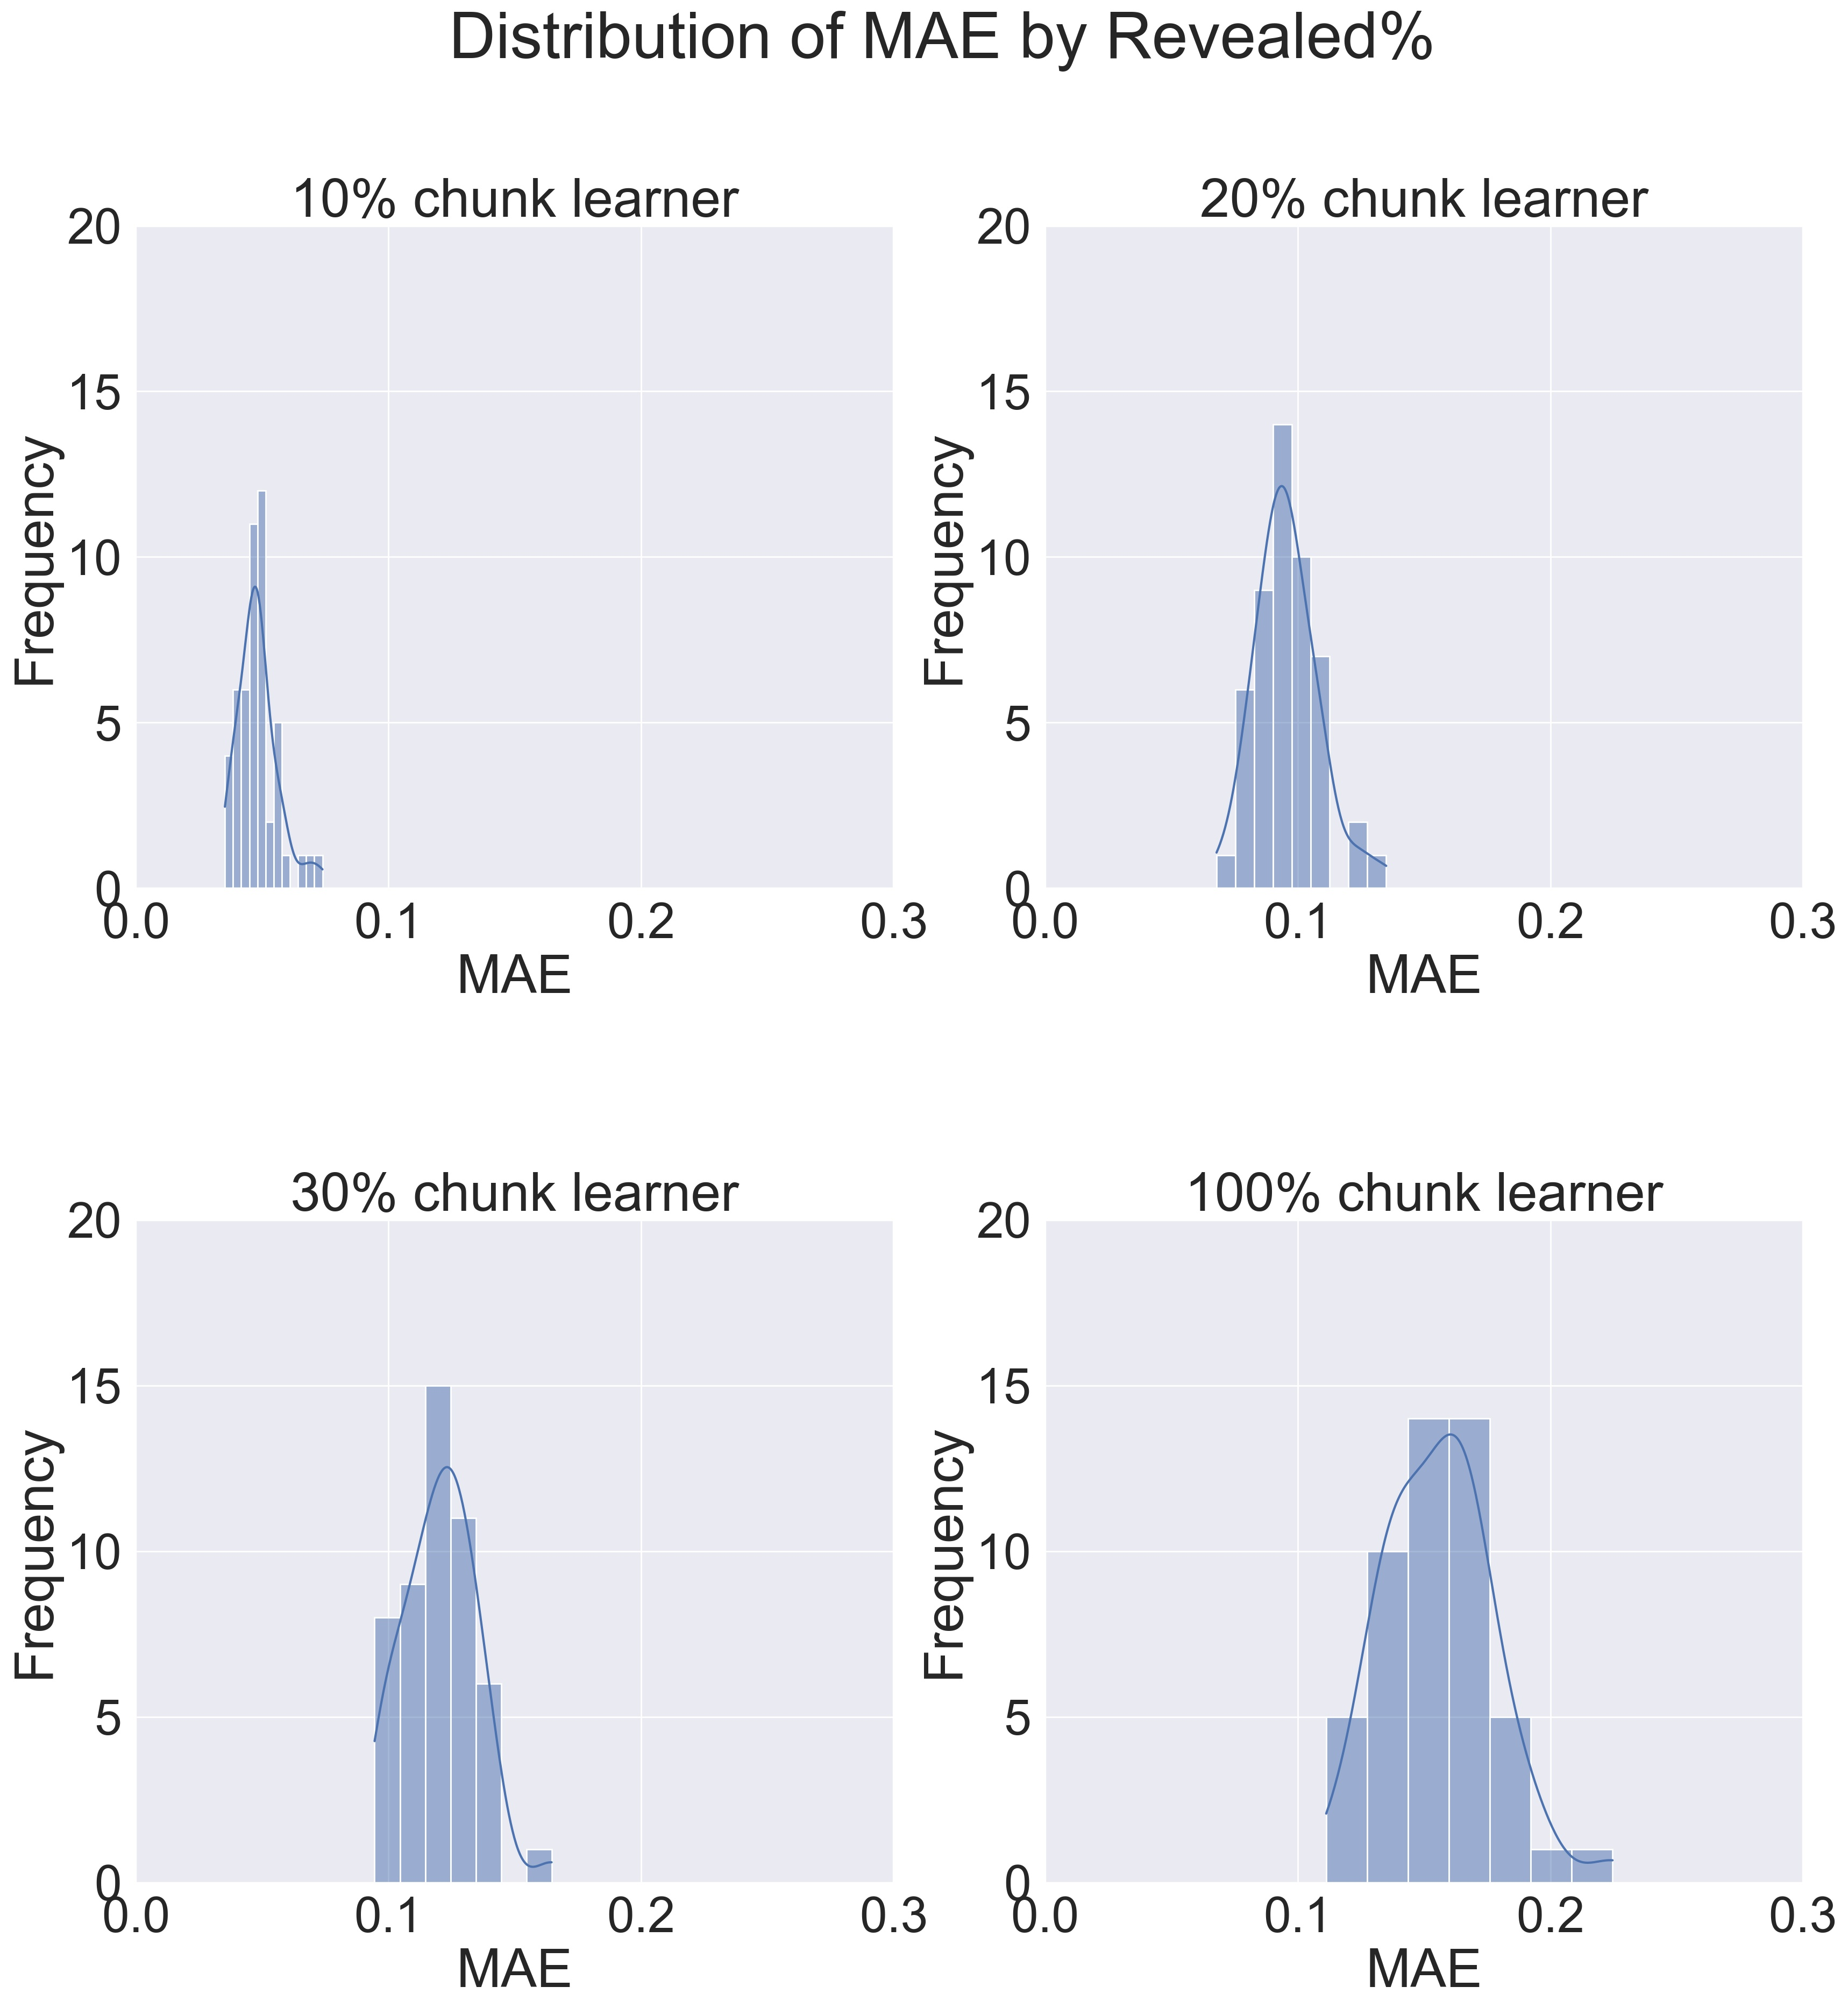
\includegraphics[width=\textwidth]{./Chapters/06 Results/hist_mae.jpg}
        \centering
        \caption{Histograms for distribution of MAE per chunk over 50 runs}
    \end{figure}


  \section{Which features contribute the most to the F-Score Prediction ?}
    \begin{figure} [!htb]
        \centering
        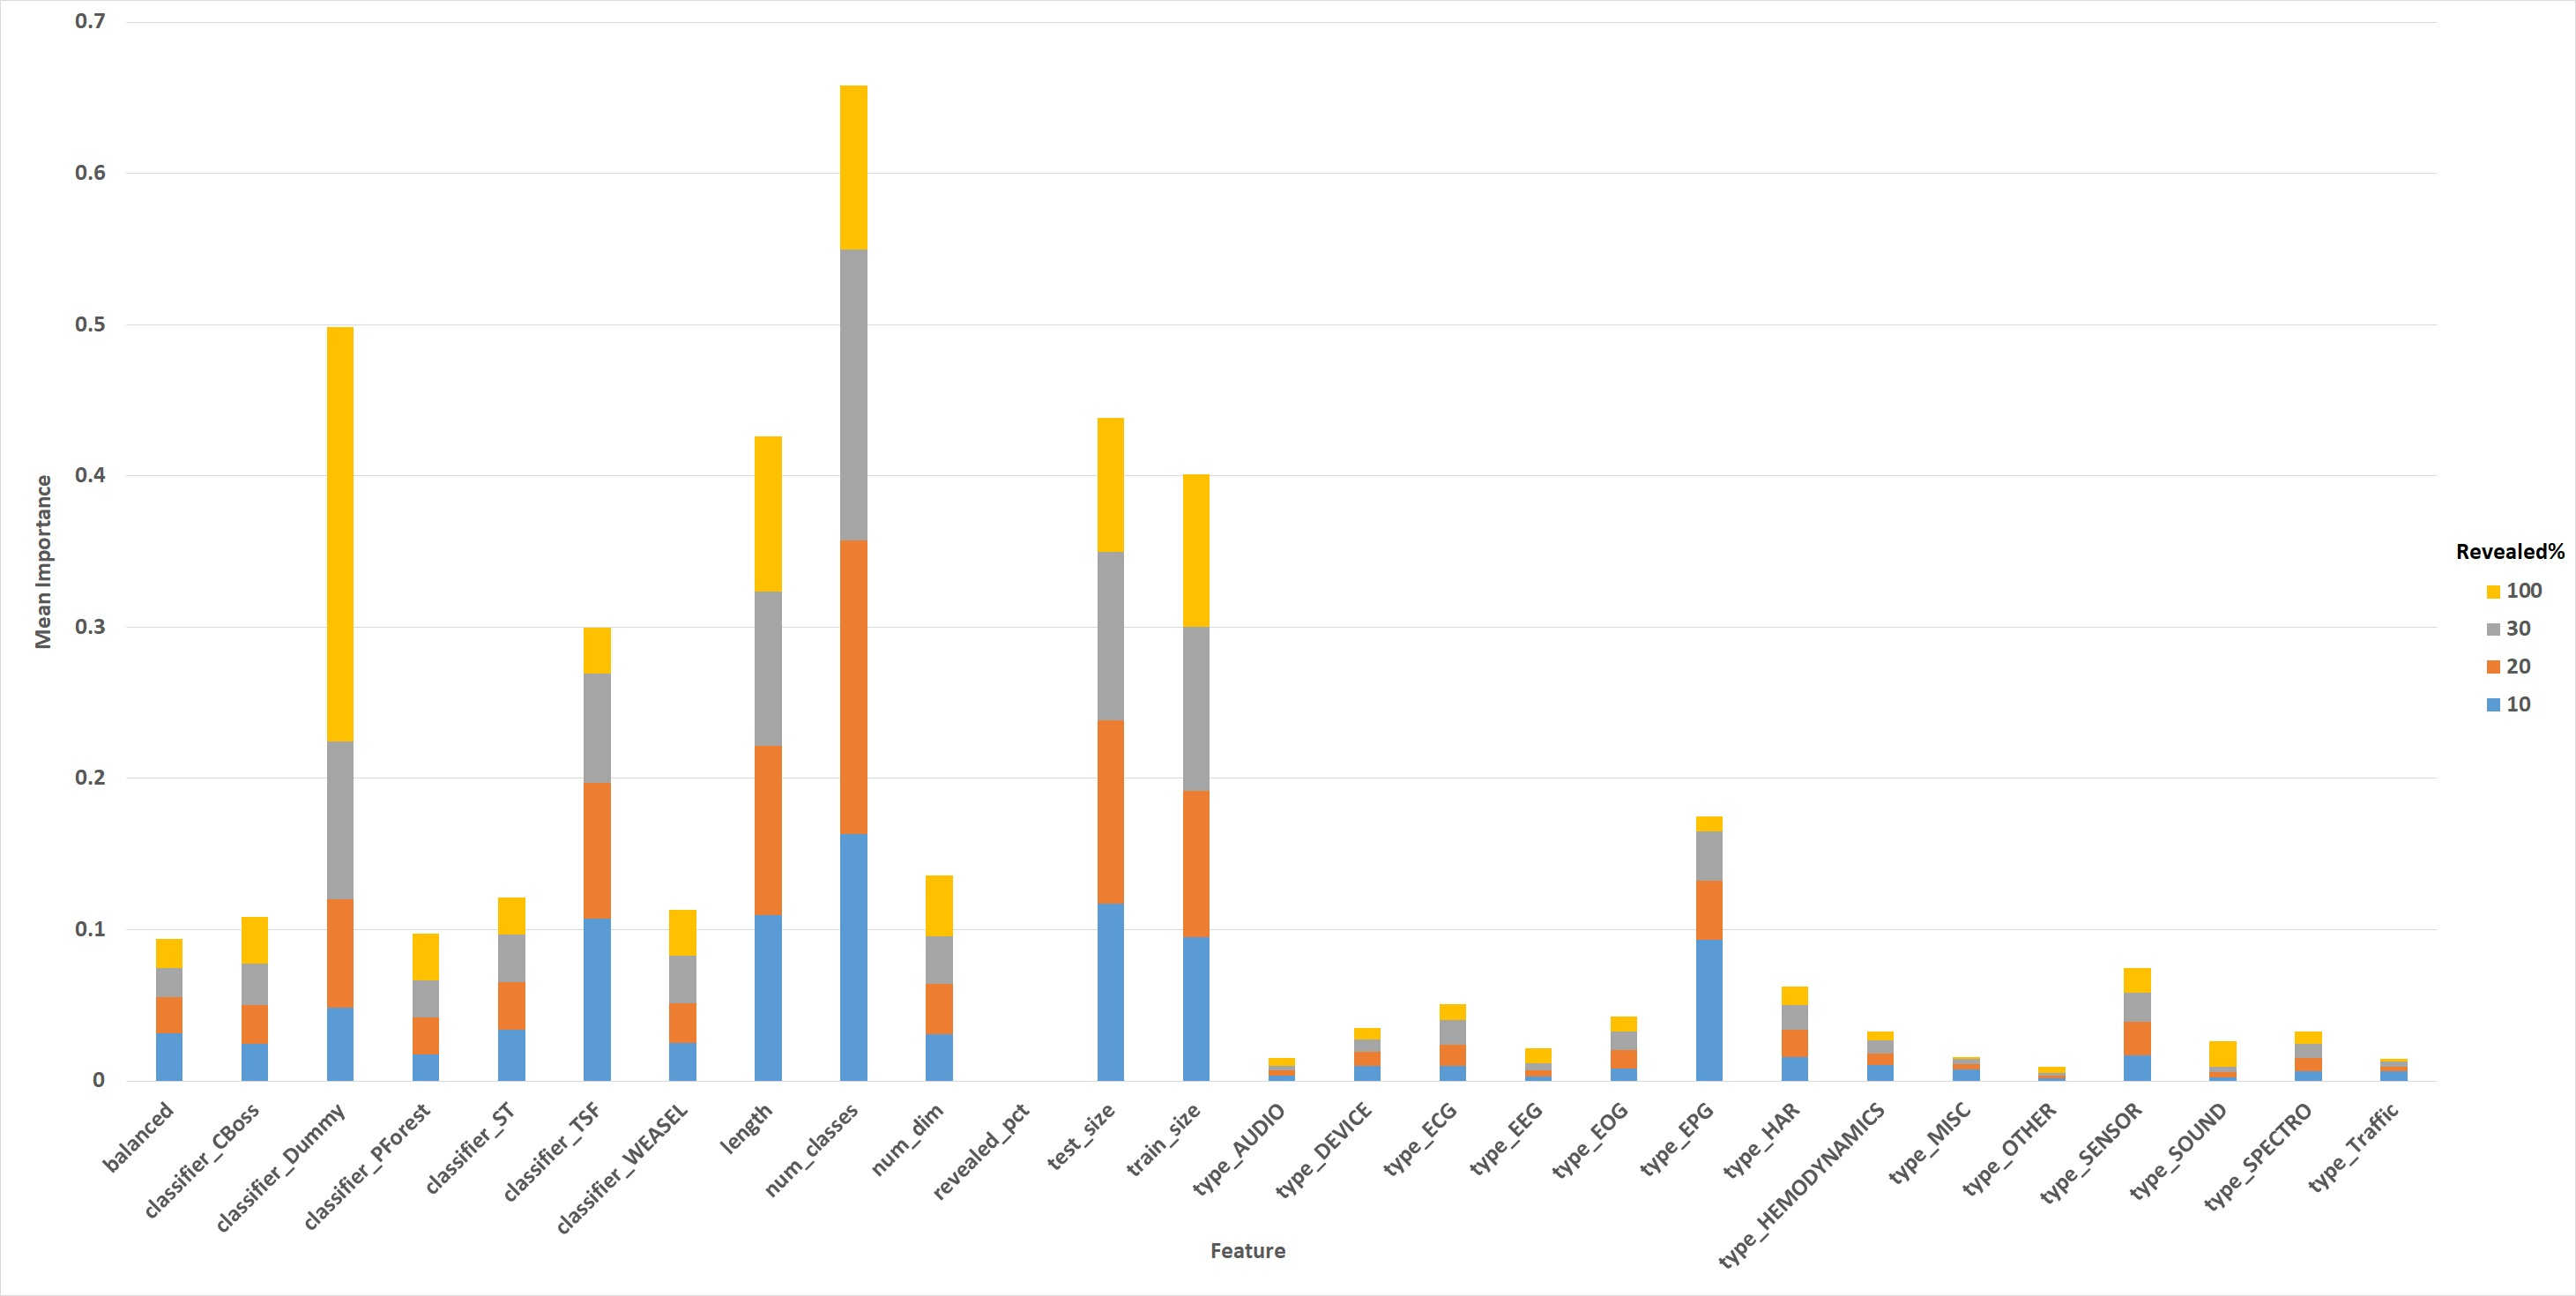
\includegraphics[width=\textwidth]{./Chapters/06 Results/Feature_Importance_stacked.jpg}
        \caption{Mean Feature Importance stacked by chunk}
    \end{figure}

  \section{Are the final recommendations of the framework consistent with actual results ?}
  
  \begin{longtable}{ |c|c|c|c|c|c|c|c|c|c| }
    \textbf{\#Seed} & \textbf{Revealed\%} & \textbf{\#Instances} & \textbf{TP} & \textbf{TN} & \textbf{FP} & \textbf{FN} & \textbf{Accuracy} & \textbf{Precision} & \textbf{Recall} \\ [0.5ex]
    \hline
    \endfirsthead % <-- This denotes the end of the header, which will be shown on the first page only
    \hline
    \textbf{\#Seed} & \textbf{Revealed\%} & \textbf{\#Instances} & \textbf{TP} & \textbf{TN} & \textbf{FP} & \textbf{FN} & \textbf{Accuracy} & \textbf{Precision} & \textbf{Recall} \\ [0.5ex]
    \hline
    \endhead
            0 & 10 & 81 & 47 & 15 & 19 & 0 & 0.77 & 0.71 & 1.00 \\ \hline
            0 & 20 & 81 & 56 & 16 & 9 & 0 & 0.89 & 0.86 & 1.00 \\ \hline
            0 & 30 & 80 & 60 & 15 & 5 & 0 & 0.94 & 0.92 & 1.00 \\ \hline
            0 & 100 & 80 & 65 & 15 & 0 & 0 & 1.00 & 1.00 & 1.00 \\ \hline
            1 & 10 & 85 & 44 & 16 & 24 & 1 & 0.71 & 0.65 & 0.98 \\ \hline
            1 & 20 & 85 & 54 & 15 & 16 & 0 & 0.81 & 0.77 & 1.00 \\ \hline
            1 & 30 & 84 & 54 & 15 & 15 & 0 & 0.82 & 0.78 & 1.00 \\ \hline
            1 & 100 & 83 & 59 & 15 & 9 & 0 & 0.89 & 0.87 & 1.00 \\ \hline
            2 & 10 & 81 & 46 & 16 & 18 & 1 & 0.77 & 0.72 & 0.98 \\ \hline
            2 & 20 & 81 & 56 & 15 & 10 & 0 & 0.88 & 0.85 & 1.00 \\ \hline
            2 & 30 & 81 & 57 & 15 & 9 & 0 & 0.89 & 0.86 & 1.00 \\ \hline
            2 & 100 & 81 & 65 & 15 & 1 & 0 & 0.99 & 0.98 & 1.00 \\ \hline
            3 & 10 & 83 & 48 & 15 & 18 & 2 & 0.76 & 0.73 & 0.96 \\ \hline
            3 & 20 & 83 & 52 & 15 & 16 & 0 & 0.81 & 0.76 & 1.00 \\ \hline
            3 & 30 & 82 & 54 & 16 & 9 & 3 & 0.85 & 0.86 & 0.95 \\ \hline
            3 & 100 & 82 & 63 & 15 & 4 & 0 & 0.95 & 0.94 & 1.00 \\ \hline
            4 & 10 & 83 & 50 & 16 & 17 & 0 & 0.80 & 0.75 & 1.00 \\ \hline
            4 & 20 & 83 & 52 & 15 & 16 & 0 & 0.81 & 0.76 & 1.00 \\ \hline
            4 & 30 & 83 & 58 & 15 & 10 & 0 & 0.88 & 0.85 & 1.00 \\ \hline
            4 & 100 & 82 & 66 & 15 & 1 & 0 & 0.99 & 0.99 & 1.00 \\ \hline
            5 & 10 & 80 & 43 & 17 & 20 & 0 & 0.75 & 0.68 & 1.00 \\ \hline
            5 & 20 & 80 & 52 & 16 & 12 & 0 & 0.85 & 0.81 & 1.00 \\ \hline
            5 & 30 & 79 & 57 & 15 & 7 & 0 & 0.91 & 0.89 & 1.00 \\ \hline
            5 & 100 & 78 & 62 & 15 & 1 & 0 & 0.99 & 0.98 & 1.00 \\ \hline
            6 & 10 & 78 & 39 & 15 & 24 & 0 & 0.69 & 0.62 & 1.00 \\ \hline
            6 & 20 & 78 & 52 & 15 & 11 & 0 & 0.86 & 0.83 & 1.00 \\ \hline
            6 & 30 & 78 & 53 & 15 & 10 & 0 & 0.87 & 0.84 & 1.00 \\ \hline
            6 & 100 & 77 & 57 & 15 & 5 & 0 & 0.94 & 0.92 & 1.00 \\ \hline
            7 & 10 & 84 & 41 & 20 & 16 & 7 & 0.73 & 0.72 & 0.85 \\ \hline
            7 & 20 & 84 & 62 & 15 & 7 & 0 & 0.92 & 0.90 & 1.00 \\ \hline
            7 & 30 & 84 & 61 & 15 & 8 & 0 & 0.90 & 0.88 & 1.00 \\ \hline
            7 & 100 & 83 & 67 & 15 & 1 & 0 & 0.99 & 0.99 & 1.00 \\ \hline
            8 & 10 & 79 & 34 & 17 & 27 & 1 & 0.65 & 0.56 & 0.97 \\ \hline
            8 & 20 & 79 & 44 & 15 & 20 & 0 & 0.75 & 0.69 & 1.00 \\ \hline
            8 & 30 & 79 & 48 & 16 & 15 & 0 & 0.81 & 0.76 & 1.00 \\ \hline
            8 & 100 & 79 & 55 & 15 & 9 & 0 & 0.89 & 0.86 & 1.00 \\ \hline
            9 & 10 & 80 & 39 & 15 & 26 & 0 & 0.68 & 0.60 & 1.00 \\ \hline
            9 & 20 & 79 & 48 & 15 & 16 & 0 & 0.80 & 0.75 & 1.00 \\ \hline
            9 & 30 & 78 & 53 & 15 & 10 & 0 & 0.87 & 0.84 & 1.00 \\ \hline
            9 & 100 & 77 & 56 & 15 & 6 & 0 & 0.92 & 0.90 & 1.00 \\ \hline
            10 & 10 & 84 & 53 & 16 & 14 & 1 & 0.82 & 0.79 & 0.98 \\ \hline
            10 & 20 & 84 & 56 & 15 & 13 & 0 & 0.85 & 0.81 & 1.00 \\ \hline
            10 & 30 & 83 & 61 & 15 & 7 & 0 & 0.92 & 0.90 & 1.00 \\ \hline
            10 & 100 & 82 & 62 & 15 & 5 & 0 & 0.94 & 0.93 & 1.00 \\ \hline
            11 & 10 & 81 & 42 & 21 & 18 & 0 & 0.78 & 0.70 & 1.00 \\ \hline
            11 & 20 & 81 & 52 & 15 & 14 & 0 & 0.83 & 0.79 & 1.00 \\ \hline
            11 & 30 & 80 & 56 & 15 & 9 & 0 & 0.89 & 0.86 & 1.00 \\ \hline
            11 & 100 & 80 & 65 & 15 & 0 & 0 & 1.00 & 1.00 & 1.00 \\ \hline
            12 & 10 & 82 & 46 & 16 & 20 & 0 & 0.76 & 0.70 & 1.00 \\ \hline
            12 & 20 & 81 & 45 & 15 & 21 & 0 & 0.74 & 0.68 & 1.00 \\ \hline
            12 & 30 & 81 & 52 & 15 & 14 & 0 & 0.83 & 0.79 & 1.00 \\ \hline
            12 & 100 & 80 & 60 & 15 & 5 & 0 & 0.94 & 0.92 & 1.00 \\ \hline
            13 & 10 & 80 & 42 & 20 & 16 & 2 & 0.78 & 0.72 & 0.95 \\ \hline
            13 & 20 & 80 & 34 & 19 & 9 & 18 & 0.66 & 0.79 & 0.65 \\ \hline
            13 & 30 & 79 & 52 & 15 & 12 & 0 & 0.85 & 0.81 & 1.00 \\ \hline
            13 & 100 & 79 & 60 & 15 & 4 & 0 & 0.95 & 0.94 & 1.00 \\ \hline
            14 & 10 & 78 & 45 & 17 & 13 & 3 & 0.79 & 0.78 & 0.94 \\ \hline
            14 & 20 & 78 & 51 & 15 & 12 & 0 & 0.85 & 0.81 & 1.00 \\ \hline
            14 & 30 & 77 & 53 & 15 & 9 & 0 & 0.88 & 0.85 & 1.00 \\ \hline
            14 & 100 & 77 & 60 & 15 & 2 & 0 & 0.97 & 0.97 & 1.00 \\ \hline
            15 & 10 & 81 & 39 & 15 & 23 & 4 & 0.67 & 0.63 & 0.91 \\ \hline
            15 & 20 & 81 & 47 & 15 & 19 & 0 & 0.77 & 0.71 & 1.00 \\ \hline
            15 & 30 & 81 & 53 & 15 & 13 & 0 & 0.84 & 0.80 & 1.00 \\ \hline
            15 & 100 & 80 & 58 & 15 & 7 & 0 & 0.91 & 0.89 & 1.00 \\ \hline
            16 & 10 & 83 & 46 & 20 & 15 & 2 & 0.80 & 0.75 & 0.96 \\ \hline
            16 & 20 & 83 & 48 & 15 & 19 & 1 & 0.76 & 0.72 & 0.98 \\ \hline
            16 & 30 & 82 & 57 & 16 & 9 & 0 & 0.89 & 0.86 & 1.00 \\ \hline
            16 & 100 & 79 & 61 & 15 & 3 & 0 & 0.96 & 0.95 & 1.00 \\ \hline
            17 & 10 & 73 & 37 & 15 & 21 & 0 & 0.71 & 0.64 & 1.00 \\ \hline
            17 & 20 & 73 & 46 & 15 & 11 & 1 & 0.84 & 0.81 & 0.98 \\ \hline
            17 & 30 & 72 & 44 & 18 & 4 & 6 & 0.86 & 0.92 & 0.88 \\ \hline
            17 & 100 & 69 & 50 & 16 & 3 & 0 & 0.96 & 0.94 & 1.00 \\ \hline
            18 & 10 & 78 & 43 & 18 & 11 & 6 & 0.78 & 0.80 & 0.88 \\ \hline
            18 & 20 & 78 & 51 & 15 & 12 & 0 & 0.85 & 0.81 & 1.00 \\ \hline
            18 & 30 & 78 & 55 & 15 & 7 & 1 & 0.90 & 0.89 & 0.98 \\ \hline
            18 & 100 & 77 & 62 & 15 & 0 & 0 & 1.00 & 1.00 & 1.00 \\ \hline
            19 & 10 & 81 & 40 & 16 & 25 & 0 & 0.69 & 0.62 & 1.00 \\ \hline
            19 & 20 & 80 & 45 & 18 & 15 & 2 & 0.79 & 0.75 & 0.96 \\ \hline
            19 & 30 & 80 & 52 & 17 & 11 & 0 & 0.86 & 0.83 & 1.00 \\ \hline
            19 & 100 & 79 & 55 & 15 & 9 & 0 & 0.89 & 0.86 & 1.00 \\ \hline
            20 & 10 & 78 & 45 & 16 & 15 & 2 & 0.78 & 0.75 & 0.96 \\ \hline
            20 & 20 & 78 & 50 & 15 & 13 & 0 & 0.83 & 0.79 & 1.00 \\ \hline
            20 & 30 & 78 & 52 & 15 & 11 & 0 & 0.86 & 0.83 & 1.00 \\ \hline
            20 & 100 & 78 & 63 & 15 & 0 & 0 & 1.00 & 1.00 & 1.00 \\ \hline
            21 & 10 & 84 & 47 & 20 & 15 & 2 & 0.80 & 0.76 & 0.96 \\ \hline
            21 & 20 & 84 & 50 & 15 & 18 & 1 & 0.77 & 0.74 & 0.98 \\ \hline
            21 & 30 & 83 & 59 & 15 & 9 & 0 & 0.89 & 0.87 & 1.00 \\ \hline
            21 & 100 & 81 & 62 & 15 & 4 & 0 & 0.95 & 0.94 & 1.00 \\ \hline
            22 & 10 & 76 & 38 & 16 & 22 & 0 & 0.71 & 0.63 & 1.00 \\ \hline
            22 & 20 & 75 & 44 & 15 & 16 & 0 & 0.79 & 0.73 & 1.00 \\ \hline
            22 & 30 & 74 & 45 & 15 & 14 & 0 & 0.81 & 0.76 & 1.00 \\ \hline
            22 & 100 & 74 & 53 & 15 & 6 & 0 & 0.92 & 0.90 & 1.00 \\ \hline
            23 & 10 & 79 & 38 & 16 & 25 & 0 & 0.68 & 0.60 & 1.00 \\ \hline
            23 & 20 & 79 & 46 & 15 & 18 & 0 & 0.77 & 0.72 & 1.00 \\ \hline
            23 & 30 & 79 & 52 & 15 & 12 & 0 & 0.85 & 0.81 & 1.00 \\ \hline
            23 & 100 & 77 & 61 & 15 & 1 & 0 & 0.99 & 0.98 & 1.00 \\ \hline
            24 & 10 & 78 & 39 & 22 & 15 & 2 & 0.78 & 0.72 & 0.95 \\ \hline
            24 & 20 & 78 & 47 & 15 & 16 & 0 & 0.79 & 0.75 & 1.00 \\ \hline
            24 & 30 & 78 & 48 & 15 & 15 & 0 & 0.81 & 0.76 & 1.00 \\ \hline
            24 & 100 & 78 & 59 & 15 & 4 & 0 & 0.95 & 0.94 & 1.00 \\ \hline
            25 & 10 & 87 & 41 & 19 & 25 & 2 & 0.69 & 0.62 & 0.95 \\ \hline
            25 & 20 & 87 & 52 & 16 & 15 & 4 & 0.78 & 0.78 & 0.93 \\ \hline
            25 & 30 & 87 & 51 & 17 & 9 & 10 & 0.78 & 0.85 & 0.84 \\ \hline
            25 & 100 & 87 & 67 & 15 & 5 & 0 & 0.94 & 0.93 & 1.00 \\ \hline
            26 & 10 & 83 & 53 & 18 & 12 & 0 & 0.86 & 0.82 & 1.00 \\ \hline
            26 & 20 & 83 & 60 & 15 & 8 & 0 & 0.90 & 0.88 & 1.00 \\ \hline
            26 & 30 & 83 & 62 & 15 & 6 & 0 & 0.93 & 0.91 & 1.00 \\ \hline
            26 & 100 & 83 & 68 & 15 & 0 & 0 & 1.00 & 1.00 & 1.00 \\ \hline
            27 & 10 & 81 & 46 & 19 & 16 & 0 & 0.80 & 0.74 & 1.00 \\ \hline
            27 & 20 & 81 & 52 & 15 & 14 & 0 & 0.83 & 0.79 & 1.00 \\ \hline
            27 & 30 & 81 & 55 & 15 & 11 & 0 & 0.86 & 0.83 & 1.00 \\ \hline
            27 & 100 & 81 & 66 & 15 & 0 & 0 & 1.00 & 1.00 & 1.00 \\ \hline
            28 & 10 & 79 & 46 & 15 & 17 & 1 & 0.77 & 0.73 & 0.98 \\ \hline
            28 & 20 & 79 & 50 & 15 & 13 & 1 & 0.82 & 0.79 & 0.98 \\ \hline
            28 & 30 & 77 & 53 & 15 & 9 & 0 & 0.88 & 0.85 & 1.00 \\ \hline
            28 & 100 & 74 & 56 & 15 & 3 & 0 & 0.96 & 0.95 & 1.00 \\ \hline
            29 & 10 & 83 & 43 & 16 & 24 & 0 & 0.71 & 0.64 & 1.00 \\ \hline
            29 & 20 & 82 & 50 & 15 & 17 & 0 & 0.79 & 0.75 & 1.00 \\ \hline
            29 & 30 & 81 & 55 & 15 & 11 & 0 & 0.86 & 0.83 & 1.00 \\ \hline
            29 & 100 & 81 & 64 & 15 & 2 & 0 & 0.98 & 0.97 & 1.00 \\ \hline
            30 & 10 & 82 & 46 & 16 & 19 & 1 & 0.76 & 0.71 & 0.98 \\ \hline
            30 & 20 & 82 & 55 & 15 & 12 & 0 & 0.85 & 0.82 & 1.00 \\ \hline
            30 & 30 & 81 & 54 & 15 & 12 & 0 & 0.85 & 0.82 & 1.00 \\ \hline
            30 & 100 & 79 & 59 & 15 & 5 & 0 & 0.94 & 0.92 & 1.00 \\ \hline
            31 & 10 & 82 & 42 & 17 & 23 & 0 & 0.72 & 0.65 & 1.00 \\ \hline
            31 & 20 & 82 & 46 & 15 & 21 & 0 & 0.74 & 0.69 & 1.00 \\ \hline
            31 & 30 & 82 & 49 & 15 & 18 & 0 & 0.78 & 0.73 & 1.00 \\ \hline
            31 & 100 & 81 & 57 & 15 & 9 & 0 & 0.89 & 0.86 & 1.00 \\ \hline
            32 & 10 & 83 & 17 & 29 & 1 & 36 & 0.55 & 0.94 & 0.32 \\ \hline
            32 & 20 & 82 & 47 & 17 & 9 & 9 & 0.78 & 0.84 & 0.84 \\ \hline
            32 & 30 & 81 & 55 & 15 & 11 & 0 & 0.86 & 0.83 & 1.00 \\ \hline
            32 & 100 & 80 & 64 & 15 & 1 & 0 & 0.99 & 0.98 & 1.00 \\ \hline
            33 & 10 & 81 & 40 & 18 & 21 & 2 & 0.72 & 0.66 & 0.95 \\ \hline
            33 & 20 & 81 & 48 & 15 & 18 & 0 & 0.78 & 0.73 & 1.00 \\ \hline
            33 & 30 & 81 & 52 & 15 & 14 & 0 & 0.83 & 0.79 & 1.00 \\ \hline
            33 & 100 & 81 & 66 & 15 & 0 & 0 & 1.00 & 1.00 & 1.00 \\ \hline
            34 & 10 & 77 & 39 & 17 & 19 & 2 & 0.73 & 0.67 & 0.95 \\ \hline
            34 & 20 & 77 & 44 & 16 & 11 & 6 & 0.78 & 0.80 & 0.88 \\ \hline
            34 & 30 & 77 & 55 & 15 & 7 & 0 & 0.91 & 0.89 & 1.00 \\ \hline
            34 & 100 & 77 & 61 & 15 & 1 & 0 & 0.99 & 0.98 & 1.00 \\ \hline
            35 & 10 & 82 & 45 & 18 & 18 & 1 & 0.77 & 0.71 & 0.98 \\ \hline
            35 & 20 & 82 & 57 & 15 & 10 & 0 & 0.88 & 0.85 & 1.00 \\ \hline
            35 & 30 & 82 & 59 & 15 & 8 & 0 & 0.90 & 0.88 & 1.00 \\ \hline
            35 & 100 & 82 & 67 & 15 & 0 & 0 & 1.00 & 1.00 & 1.00 \\ \hline
            36 & 10 & 75 & 34 & 18 & 21 & 2 & 0.69 & 0.62 & 0.94 \\ \hline
            36 & 20 & 75 & 31 & 23 & 5 & 16 & 0.72 & 0.86 & 0.66 \\ \hline
            36 & 30 & 75 & 48 & 15 & 12 & 0 & 0.84 & 0.80 & 1.00 \\ \hline
            36 & 100 & 73 & 53 & 15 & 5 & 0 & 0.93 & 0.91 & 1.00 \\ \hline
            37 & 10 & 84 & 45 & 16 & 22 & 1 & 0.73 & 0.67 & 0.98 \\ \hline
            37 & 20 & 84 & 50 & 15 & 19 & 0 & 0.77 & 0.72 & 1.00 \\ \hline
            37 & 30 & 84 & 53 & 17 & 13 & 1 & 0.83 & 0.80 & 0.98 \\ \hline
            37 & 100 & 84 & 69 & 15 & 0 & 0 & 1.00 & 1.00 & 1.00 \\ \hline
            38 & 10 & 84 & 40 & 17 & 27 & 0 & 0.68 & 0.60 & 1.00 \\ \hline
            38 & 20 & 83 & 50 & 15 & 18 & 0 & 0.78 & 0.74 & 1.00 \\ \hline
            38 & 30 & 81 & 54 & 15 & 12 & 0 & 0.85 & 0.82 & 1.00 \\ \hline
            38 & 100 & 81 & 60 & 15 & 6 & 0 & 0.93 & 0.91 & 1.00 \\ \hline
            39 & 10 & 77 & 40 & 17 & 18 & 2 & 0.74 & 0.69 & 0.95 \\ \hline
            39 & 20 & 77 & 46 & 15 & 15 & 1 & 0.79 & 0.75 & 0.98 \\ \hline
            39 & 30 & 77 & 51 & 15 & 11 & 0 & 0.86 & 0.82 & 1.00 \\ \hline
            39 & 100 & 75 & 55 & 15 & 5 & 0 & 0.93 & 0.92 & 1.00 \\ \hline
            40 & 10 & 81 & 42 & 19 & 20 & 0 & 0.75 & 0.68 & 1.00 \\ \hline
            40 & 20 & 80 & 52 & 15 & 13 & 0 & 0.84 & 0.80 & 1.00 \\ \hline
            40 & 30 & 80 & 56 & 15 & 9 & 0 & 0.89 & 0.86 & 1.00 \\ \hline
            40 & 100 & 80 & 63 & 15 & 2 & 0 & 0.98 & 0.97 & 1.00 \\ \hline
            41 & 10 & 76 & 36 & 16 & 22 & 2 & 0.68 & 0.62 & 0.95 \\ \hline
            41 & 20 & 76 & 38 & 18 & 16 & 4 & 0.74 & 0.70 & 0.90 \\ \hline
            41 & 30 & 76 & 46 & 15 & 15 & 0 & 0.80 & 0.75 & 1.00 \\ \hline
            41 & 100 & 76 & 56 & 15 & 5 & 0 & 0.93 & 0.92 & 1.00 \\ \hline
            42 & 10 & 86 & 41 & 16 & 29 & 0 & 0.66 & 0.59 & 1.00 \\ \hline
            42 & 20 & 86 & 51 & 15 & 20 & 0 & 0.77 & 0.72 & 1.00 \\ \hline
            42 & 30 & 86 & 54 & 15 & 17 & 0 & 0.80 & 0.76 & 1.00 \\ \hline
            42 & 100 & 85 & 65 & 15 & 5 & 0 & 0.94 & 0.93 & 1.00 \\ \hline
            43 & 10 & 85 & 51 & 17 & 17 & 0 & 0.80 & 0.75 & 1.00 \\ \hline
            43 & 20 & 85 & 54 & 18 & 8 & 5 & 0.85 & 0.87 & 0.92 \\ \hline
            43 & 30 & 84 & 62 & 15 & 7 & 0 & 0.92 & 0.90 & 1.00 \\ \hline
            43 & 100 & 83 & 67 & 15 & 1 & 0 & 0.99 & 0.99 & 1.00 \\ \hline
            44 & 10 & 77 & 39 & 16 & 22 & 0 & 0.71 & 0.64 & 1.00 \\ \hline
            44 & 20 & 77 & 17 & 25 & 10 & 25 & 0.55 & 0.63 & 0.40 \\ \hline
            44 & 30 & 77 & 47 & 15 & 15 & 0 & 0.81 & 0.76 & 1.00 \\ \hline
            44 & 100 & 73 & 55 & 15 & 3 & 0 & 0.96 & 0.95 & 1.00 \\ \hline
            45 & 10 & 78 & 39 & 20 & 10 & 9 & 0.76 & 0.80 & 0.81 \\ \hline
            45 & 20 & 78 & 52 & 15 & 11 & 0 & 0.86 & 0.83 & 1.00 \\ \hline
            45 & 30 & 77 & 56 & 15 & 6 & 0 & 0.92 & 0.90 & 1.00 \\ \hline
            45 & 100 & 77 & 58 & 15 & 4 & 0 & 0.95 & 0.94 & 1.00 \\ \hline
            46 & 10 & 83 & 41 & 19 & 19 & 4 & 0.72 & 0.68 & 0.91 \\ \hline
            46 & 20 & 83 & 51 & 15 & 15 & 2 & 0.80 & 0.77 & 0.96 \\ \hline
            46 & 30 & 82 & 54 & 15 & 13 & 0 & 0.84 & 0.81 & 1.00 \\ \hline
            46 & 100 & 81 & 59 & 15 & 7 & 0 & 0.91 & 0.89 & 1.00 \\ \hline
            47 & 10 & 85 & 46 & 15 & 24 & 0 & 0.72 & 0.66 & 1.00 \\ \hline
            47 & 20 & 85 & 54 & 15 & 15 & 1 & 0.81 & 0.78 & 0.98 \\ \hline
            47 & 30 & 85 & 58 & 15 & 12 & 0 & 0.86 & 0.83 & 1.00 \\ \hline
            47 & 100 & 85 & 65 & 15 & 5 & 0 & 0.94 & 0.93 & 1.00 \\ \hline
            48 & 10 & 84 & 41 & 22 & 15 & 6 & 0.75 & 0.73 & 0.87 \\ \hline
            48 & 20 & 84 & 55 & 15 & 14 & 0 & 0.83 & 0.80 & 1.00 \\ \hline
            48 & 30 & 84 & 58 & 15 & 11 & 0 & 0.87 & 0.84 & 1.00 \\ \hline
            48 & 100 & 82 & 66 & 15 & 1 & 0 & 0.99 & 0.99 & 1.00 \\ \hline
            49 & 10 & 82 & 33 & 27 & 16 & 6 & 0.73 & 0.67 & 0.85 \\ \hline
            49 & 20 & 81 & 51 & 15 & 15 & 0 & 0.81 & 0.77 & 1.00 \\ \hline
            49 & 30 & 81 & 54 & 15 & 12 & 0 & 0.85 & 0.82 & 1.00 \\ \hline
            49 & 100 & 80 & 64 & 15 & 1 & 0 & 0.99 & 0.98 & 1.00 \\ \hline
    \caption{Confusion Matrix of chunk learners in predicting good and bad classifiers per chunk over 50 runs}
\end{longtable}